\documentclass[11pt,a4paper]{article}

\usepackage[a4paper,margin=2.2cm]{geometry}
\usepackage{amsmath}
\usepackage{amssymb}
\usepackage{booktabs}
\usepackage{graphicx}
\usepackage{microtype}
\usepackage[colorlinks=true,linkcolor=blue,urlcolor=blue,citecolor=blue]{hyperref}

\graphicspath{{figs/}}

\newcommand{\arxiv}[1]{\href{https://arxiv.org/abs/#1}{arXiv:#1}}
\newcommand{\code}[1]{\texttt{\detokenize{#1}}}
\newcommand{\mW}{m_W}
\newcommand{\GammaW}{\Gamma_W}
\newcommand{\GammaWzero}{\Gamma_W^{(0)}}
\newcommand{\sqrts}{\sqrt{s}}
\newcommand{\munuqq}{\mu^-\bar\nu_\mu u\bar d}
\newcommand{\fb}{\ensuremath{\,\mathrm{fb}}}
\newcommand{\GeV}{\ensuremath{\,\mathrm{GeV}}}
\newcommand{\MeV}{\ensuremath{\,\mathrm{MeV}}}
\newcommand{\pb}{\ensuremath{\,\mathrm{pb}}}

\title{BFS implementation report\\
\large WW threshold cross section for the FCC-ee $\mW$ measurement}
\author{Matteo Defranchis}
\date{\today}

\begin{document}
\maketitle

\begin{abstract}
We document the BFS unstable-particle EFT cross-section chain implemented
for the FCC-ee $W$-pair threshold scan. The chain combines the full Born
expansion through $N^{3/2}\text{LO}_\text{EFT}$, the NLO loop corrections
(hard$+$soft$+$collinear, NLO Coulomb, EW decay), the dominant NNLO
$\sigma^{(3/2)}_\text{LR}$ contributions of eq.~(49) of \cite{BFSnnlo},
a multiplicative QCD width correction $\delta_\text{QCD}$, a Whizard
exact-Born anchor on the Born sum, and an $\mathrm{LL{+}exp}$ ISR
convolution in the BETA scheme. Every numerical table in this report
corresponds to a script in the repository (cf.~\code{report/README.md});
all numbers shown are reproduced verbatim from the current code.
\end{abstract}

\tableofcontents

% ---------------------------------------------------------------
\section{Goal and scope}
% ---------------------------------------------------------------

The FCC-ee threshold scan aims at $\sim$MeV-precision $\mW$ from
$e^+e^-\to W^+W^- \to$ 4 fermions in the energy window
$\sqrts\in[157,163]\GeV$. With $\sim 10^6$ events per scan point this
requires a theory prediction whose residual uncertainty on
$\mathrm{d}\sigma/\mathrm{d}\mW$ is well below $0.1\%/\!\MeV$. Two parallel
calculations are foreseen: an in-process analytic implementation, and a
WHIZARD-based parallel calculation (still to be wired). This report
documents the analytic implementation, which is the BFS \emph{unstable-W}
EFT expansion of Beneke, Falgari, Schwinn and collaborators, established
in their NLO paper~\cite{BFSnlo} and the dominant-NNLO
follow-up~\cite{BFSnnlo}.

We focus on
\begin{itemize}
\item the equations actually evaluated by the code (section \ref{sec:impl});
\item the round-trips that confirm the implementation reproduces every
      table of the two BFS papers we currently rely on (section \ref{sec:val}).
\end{itemize}
Limitations and open items are collected in section \ref{sec:limits}.

% ---------------------------------------------------------------
\section{The BFS unstable-particle EFT in one page}
% ---------------------------------------------------------------

BFS organise the threshold cross section as a double expansion in the
electroweak coupling $\alpha$ and the resonance scaling
$\delta\sim\GammaW/\mW \sim v^2$, where $v$ is the non-relativistic
$W$-velocity. Counting $\delta\sim\alpha$, the partonic four-fermion
cross section reads
\begin{equation}
\hat\sigma(s) \;=\; \sigma^{(0)} \;+\; \sigma^{(1/2)} \;+\; \sigma^{(1)}
   \;+\; \sigma^{(3/2)} \;+\; \mathcal{O}(\delta^2),
\label{eq:bfs-expansion}
\end{equation}
where $\sigma^{(p/2)}$ collects everything of relative order $\delta^{p/2}$
($p\!=\!0,1,2,3$ are usually called $\mathrm{LO}$, $\mathrm{N^{1/2}LO}$,
$\mathrm{NLO}$, $\mathrm{N^{3/2}LO}$ in the EFT counting). Going beyond
$N^{3/2}\text{LO}_\text{EFT}$ requires the dominant pieces of
$\sigma^{(2)}$ identified in Ref.~\cite{BFSnnlo} (``NNLO'' in this
report to match the BFS-NNLO paper convention).

The natural BFS quantity is the LR-helicity cross section for the
\emph{specific} channel $e^+e^-\to\munuqq$,
\begin{equation}
\sigma_{\rm LR}^{(p/2)}(s;\mW,\GammaW),
\end{equation}
in which the leptonic and hadronic $W$ branching fractions are encoded
through an explicit prefactor proportional to $1/27$ (BFS line 1130).
For the analysis we need the unpolarised initial state and the inclusive
$\mu\nu q\bar q$ final state, both of which are derived from
$\sigma_\mathrm{LR}^{(p/2)}$ by trivial helicity and flavour multipliers
(section~\ref{sec:born}).

When the propagator width $\GammaW$ is the NLO+QCD value rather than the
LO theoretical width $\GammaWzero$, the explicit $1/27$ in the BFS Born
formulae must be replaced by $(\GammaWzero/\GammaW)^2 / 27$ for the doubly
resonant piece and by $(\GammaWzero/\GammaW)/27$ for the singly resonant
piece (BFS section~6.1 / eq.~(83)). The code applies this BR correction
component-by-component, see section~\ref{sec:born}.

% ---------------------------------------------------------------
\section{Implementation}\label{sec:impl}
% ---------------------------------------------------------------

\subsection{Code organisation}\label{sec:codeorg}

The BFS chain lives under \code{framework/process/ww/xsec_calculator/}:
\begin{description}
\item[\code{eft_xsec.py}] EW couplings ($s_W^2$ OS, $\alpha_{G_\mu}(\mW)$),
   the BFS-paper reference constants, the partonic specific-channel
   driver $\code{sigma\_partonic\_munuqq}$, and the $K_C$ Coulomb
   resummation factor.
\item[\code{bfs_eft.py}] All closed-form BFS contributions: Born
   expansion (eqs.~17, 33, 37, 38, 39, 40 of \cite{BFSnlo}), NLO
   loop corrections (HSC bracket, NLO Coulomb eq.~62, EW decay), and
   the dominant NNLO pieces (eq.~49 of \cite{BFSnnlo}). Also the
   Whizard-anchor factor and the $\delta_\text{QCD}$ multiplier.
\item[\code{isr.py}] LL+exp ISR convolution in the BETA scheme,
   in two forms: a single-convolution shortcut and the BFS-style
   two-leg double convolution.
\end{description}

The public assembly functions are:
\begin{description}
\item[$\code{sigma\_BFS\_specific\_munuud\_pb}(s,\mW,\GammaW;\ldots)$]
   sums all enabled BFS pieces for the specific channel $\munuqq$.
\item[$\code{sigma\_observed\_munuqq}(\sqrts,\mW,\GammaW;\ldots)$]
   ISR-convoluted observed cross section, $\mu\nu q\bar q$ or per
   channel, exposing the chain via keyword toggles.
\end{description}
The defaults of \code{sigma_observed_munuqq} are the project's ``best
calculation'': full BFS Born $+$ NLO loops $+$ NNLO $+$ $\delta_\text{QCD}$
$+$ Whizard anchor $+$ single-convolution LL+exp ISR (cf.~section
\ref{sec:isr}).

\subsection{Born expansion}\label{sec:born}

The Born sum implemented in \code{bfs_eft.py} for the specific channel
$\munuqq$ is
\begin{equation}
\sigma_\mathrm{LR}^\text{Born} \;=\;
\sigma_\mathrm{LR}^{(0)} \,+\, \sigma_\mathrm{LR}^{(1/2)} \,+\,
\sigma_\mathrm{LR}^{(1)} \,+\, \sigma_\mathrm{LR}^{(3/2),a},
\end{equation}
plus the analogous $RL$ sum (no $RL^{(0)}$ contribution: see
Ref.~\cite{BFSnlo} section 4.1). The five pieces correspond to:
\begin{itemize}
\item $\sigma_\mathrm{LR}^{(0)}$ — doubly resonant LO, eq.~(17) of
   \cite{BFSnlo}, evaluated with the complex-velocity
   $\beta(s)=\sqrt{(s-4\mW^2+i\Gamma_W\,\cdot 2\mW)/s}$. Coded in
   \code{sigma_LR0_specific_pb}.
\item $\sigma_\mathrm{LR,RL}^{(1)}$ — NLO subleading potential
   (single-Coulomb-exchange residue), eq.~(33). Note that the
   $\GammaW^\text{NLO}$ correction to the potential cross section (the
   $\GammaW \to \GammaW(1+\delta_\text{decay}^\text{(1,ew)})$ shift
   inside eq.~33) is folded into our NLO-decay term and \emph{not}
   here, to avoid double counting; \code{sigma_LR_RL_NLO_potential_specific_pb}
   takes an explicit $\GammaW^\text{NLO}$ argument that defaults to zero.
\item $\sigma_\mathrm{LR,RL}^{(1/2)}$ — hard non-resonant, eqs.~(37)+(38)
   plus the appendix-A $C^f_{h_i,h}\,K^f_{h_i}$ coefficients for $h_4$–$h_7$.
   Coded in \code{sigma_LR_RL_half_specific_pb}; the $K$-coefficients
   $K^f_{h_4}=\{-0.266477, +0.190394\}$ etc.\ are pasted from BFS lines
   3116–3148.
\item $\sigma_\mathrm{LR,RL}^{(3/2),a}$ — energy-dependent $N^{3/2}$LO,
   eqs.~(39)+(40), in \code{sigma_LR_RL_three_half_a_specific_pb}.
\end{itemize}

\paragraph{Pieces deliberately omitted.}
\begin{itemize}
\item $\sigma^{(3/2),b}$ (eq.~41) — the paper estimates its size at
   $\lesssim 2\fb$, energy-independent. Empirically our Born sum
   reproduces the BFS Table~1 $N^{3/2}\mathrm{LO}_\mathrm{EFT}$ column
   to 4–5 digits at every $\sqrts$ in the scan window
   (section~\ref{sec:val-born}), which bounds the size of any missing
   piece well below $0.01\fb$.
\item $\sigma_\mathrm{RL}^{(1)}$ at NLO loop level — drops at NLO
   (Ref.~\cite{BFSnlo} section 4.1: no LR/RL helicity interference at
   one loop).
\item $\mathrm{Im}\,c_{p,\mathrm{LR}}^{(1,\mathrm{fin})}$ — paper section 4.2
   above eq.~(53): for the flavour-specific cross section only
   $\mathrm{Re}\,c_{p,\mathrm{LR}}^{(1,\mathrm{fin})}$ contributes.
\end{itemize}

\paragraph{BR-correction convention.} The BFS Born formulae carry a
$1/27$ flavour factor that assumes the LO theoretical $W$ width
$\GammaWzero(\mW)=3\alpha\,\mW/(4 s_W^2)$ in the propagator (eq.~19).
When the propagator uses an NLO+QCD width $\GammaW\neq\GammaWzero$, BFS
eq.~(83) instructs the user to multiply each piece by an appropriate
power of $\GammaWzero/\GammaW$: \emph{two} cut propagators (doubly
resonant) get $(\GammaWzero/\GammaW)^2$, \emph{one} cut propagator
(singly resonant) gets $(\GammaWzero/\GammaW)$. Our
\code{_BR_correction(\mW,\GammaW)} encodes the squared factor; the
linear vs.\ squared assignment is done by the assembly function
$\code{sigma\_BFS\_specific\_munuud\_pb}$ piece by piece. Without this
correction the BFS Table~2 prediction is $\sim$4–5\% too large.

\subsection{NLO loop corrections}\label{sec:nlo}

The NLO content of Ref.~\cite{BFSnlo} section 4 is split into three
additive pieces, all applied to $\sigma_\mathrm{LR}$ only:

\paragraph{Hard $+$ soft $+$ collinear (HSC).}
The bracket term of eq.~(\textsc{finalcross}),
\begin{equation}
\Delta\hat\sigma_\mathrm{LR}^{(1,\mathrm{HSC})} =
\frac{4\alpha^3}{27\,s_W^4 s}\,
\mathrm{Im}\!\left\{-\sqrt{z}\Big[2\ln(4z)+
\mathrm{Re}\,c_{p,\mathrm{LR}}^{(1,\mathrm{fin})} +
\tfrac{\pi^2}{4} + \tfrac{1}{2}\Big]\right\},
\quad z=-(E+i\GammaW)/\mW,\;E=\sqrts-2\mW,
\end{equation}
is the residue of the hard $+$ soft $+$ collinear corrections after all
$1/\epsilon^2$ and $1/\epsilon$ poles cancel against each other and
against the LL-ePDF scheme conversion. Coded in
\code{delta_sigma_NLO_hard_softcoll_specific_pb}. The hard matching
coefficient is $\mathrm{Re}\,c_{p,\mathrm{LR}}^{(1,\mathrm{fin})}=-10.076$
(BFS line 1797); its $\mW$ dependence is sub-percent on $\sigma^{(1,\mathrm{HSC})}$
in the fit range, see section \ref{sec:val-loops} and the
Scenario~H closure.

\paragraph{NLO Coulomb potential.}
Eq.~(62) of \cite{BFSnlo}, the $\alpha\,\alpha_\text{em}^2/s$
single-Coulomb-correction term plus the two-photon subleading piece.
Coded in \code{delta_sigma_Coulomb_NLO_specific_pb}.

\paragraph{NLO electroweak decay.}
Ref.~\cite{BFSnlo} eq.~(\textsc{delta-decay}) / eq.~(60),
\begin{equation}
\Delta\sigma_\mathrm{decay}^{(1,\mathrm{ew})} =
\Big(\Gamma_{\mu\nu}^{(1,\mathrm{ew})}/\Gamma_{\mu\nu}^{(0)} +
     \Gamma_{ud}^{(1,\mathrm{ew})}/\Gamma_{ud}^{(0)}\Big)\,
\sigma_\mathrm{LR}^{(0)},
\end{equation}
with the bracket from eq.~(\textsc{Gamma1ewFS}) evaluated with
$c_{d,\ell}^{(1,\mathrm{fin})}=-2.709$, $c_{d,h}^{(1,\mathrm{fin})}=-2.034$
(BFS line 1920). At the BFS reference parameters the bracket equals
$-0.71\%$ (purely EW; QCD content is captured by $\delta_\text{QCD}$
below — including both would double-count). Coded in
\code{delta_sigma_NLO_decay_specific_pb}.

\subsection{Dominant NNLO}\label{sec:nnlo}

The dominant $N^{3/2}\text{LO}_\text{EFT}$ partonic correction of
Ref.~\cite{BFSnnlo} eq.~(49) is the sum
\begin{equation}
\hat\sigma_\mathrm{LR}^{(3/2)} =
\Delta\hat\sigma^{(C\times[S+H])}_\mathrm{LR} +
\Delta\sigma^{(\text{NLO-}C)}_\mathrm{LR} +
\Delta\sigma^{(C\times\text{decay})}_\mathrm{LR} +
\Delta\sigma^{(C\times\text{res})}_\mathrm{LR} +
\Delta\sigma^{(C3)}_\mathrm{LR}.
\end{equation}
All five admit closed forms in the paper and are coded in
\code{bfs_eft.py}:
\begin{description}
\item[$\Delta\hat\sigma^{(C\times[S+H])}$ (eq.~34)] interference of
   single-Coulomb exchange with the soft+hard NLO corrections,
   $\propto \alpha_\mathrm{ew}^2 \alpha^2/(27 s)$, with bracket
   $9 + \pi^2/2 + 2\,\mathrm{Re}\,c_{p,\mathrm{LR}}^{(1,\mathrm{fin})}$
   times $\mathrm{Im}\,\ln(-\mathcal{E}_W/\mW)$ plus
   $2\,\mathrm{Im}\,\ln^2(-\mathcal{E}_W/\mW)$.
\item[$\Delta\sigma^{(\text{NLO-}C)}$ (eq.~39)]
   $\alpha(M_Z)$-scheme piece (photon-bubble running of $\alpha$ on the
   Coulomb photon) plus the $\alpha(M_Z)\to G_\mu$ conversion
   $\delta_{\alpha(M_Z)\to G_\mu}=4.103\,\alpha$. Uses the photon
   vacuum-polarisation sum $\sum_f C_f Q_f^2 = 20/3$ (top integrated out).
\item[$\Delta\sigma^{(C\times\text{decay})}$ (eq.~40)] same EW-decay
   bracket as $\Delta\sigma^{(1,\mathrm{ew})}_\text{decay}$ times the
   single-Coulomb piece $\Delta\sigma^{(C1)}$.
\item[$\Delta\sigma^{(C\times\text{res})}$ (eq.~48)] interference of
   residue correction and single-Coulomb exchange, $\propto
   \alpha_\mathrm{ew}^2 \alpha / (27 s) \cdot \GammaW/\mW$ times an
   $|\mathcal{E}_W|$-dependent logarithm; dominant NNLO piece above
   threshold ($\sim 1.5\fb$ at $170\GeV$).
\item[$\Delta\sigma^{(C3)}$ (eq.~11)] triple-Coulomb exchange,
   $\propto \alpha^3\,\zeta(3)\,\mathrm{Im}[-\mW/\mathcal{E}_W]$;
   tiny ($\lesssim 0.01\fb$ helicity-averaged).
\end{description}
The total NNLO impact on $\mW$ is $\sim$3\MeV{} after ISR (BFS sec.~6),
$\sim$5\MeV{} partonic. The $\hat\cdot$ on $\Delta\hat\sigma^{(C\times[S+H])}$
denotes that the IR poles have been subtracted by the LL ePDF in
$\overline{\rm MS}$ — the BFS paper instructs that this partonic piece
must be further ISR-convoluted (section~\ref{sec:val-nnlo-isr}).

\subsection{$\delta_\text{QCD}$ multiplier}\label{sec:dqcd}

The universal QCD correction to hadronic partial widths,
\begin{equation}
\delta_\text{QCD}(\alpha_s) = 1 + \frac{\alpha_s}{\pi} +
1.409\,\Big(\frac{\alpha_s}{\pi}\Big)^2,
\end{equation}
multiplies the full NLO electroweak cross section. BFS section 6.1
(lines 2622–2637) shows that doing so reproduces the QCD running of
hadronic partial widths to NNLO precision. At $\alpha_s(\mW)=0.1199$
this is $+4.0\%$. Coded in \code{delta_QCD_factor}. The QCD content of
$\delta_\text{decay}^{(1)}$ is intentionally not included in the EW
\code{delta_decay_EW_relative} to avoid double counting.

\subsection{Whizard exact-Born anchor}\label{sec:anchor}

BFS section 6.2 prescribes a final ``anchor'' to the Whizard exact 4-fermion
Born: the BFS Born EFT truncation, summed and BR-corrected, is multiplied
by
\begin{equation}
f(\sqrts,\mW,\GammaW) \;=\;
\frac{\sigma_\mathrm{Whizard}^\text{exact Born}(\sqrts,\mW,\GammaW)}
     {\sigma_\mathrm{LR}^\text{Born,BFS}(\sqrts,\mW,\GammaW)},
\end{equation}
which captures the difference between the EFT $N^{3/2}\mathrm{LO}$
truncation and the exact 4-fermion Born within the same propagator
prescription. The anchor is applied to the Born sum \emph{only}, not to
the NLO loops or NNLO additions, which are added on top per
eq.~(\textsc{finalcross}).

Two interchangeable sources for $\sigma_\mathrm{Whizard}^\text{exact Born}$
are wired in and selectable via \code{NLO\_CONFIG["whizard\_anchor\_source"]}:
\begin{itemize}
\item \texttt{spline} (default) — cubic in $\delta = \sqrts - 2\mW$ and
  linear in $\GammaW$ between the two BFS reference points
  ($\GammaW = 2.04483$ and $2.09201$~GeV) from Tables~1 and~2 of
  arXiv:0707.0773.
\item \texttt{grid} — trilinear interpolation in $(\sqrts,\mW,\GammaW)$
  on a 1295-point WHIZARD~3.1.5 scan
  ($5\,\mW \times 7\,\GammaW \times 37\,\sqrts$, $\sim$0.05\,\% MC stat
  per point) produced by the pipeline in \texttt{WW\_threshold/whizard/}.
  This is the trilinear interpolator currently wired into the fit;
  it will be superseded by the morphing scheme of
  section~\ref{sec:morphing}, which is built on a dedicated
  6363-point \texttt{grid\_fine} campaign
  ($9\,\mW \times 7\,\GammaW \times 101\,\sqrts$ at 0.1-GeV $\sqrts$
  step in $[155, 165]$~GeV, $\sim$0.008\,\% MC stat, i.e.\ 25-MeV $\mW$
  step), plus the 0.5-GeV outer wings from the highstats campaign as
  $\sqrts$-spline support beyond the fine window. A held-out
  sub-MeV ($\mW,\GammaW$) campaign at $\sim$0.005\,\% MC bounds the
  morph's interpolation bias at the fit's working resolution.
\end{itemize}
WHIZARD computes the specific channel $\mu^-\bar\nu_\mu u\bar d$ with
SM-LO partial widths fixed by the EW input scheme, so as the propagator
$\GammaW$ is scanned the implicit
$(\Gamma_\text{partial}/\GammaW)^2$ branching ratio shrinks. For the
PDG-constant BR convention used by the fit, that squeeze is undone by a
fixed BR-strip factor
$(\GammaW / \Gamma_W^{(0)}(M_W^\text{BFS,ref}))^2$ in the anchor's
numerator — fixed reference (not the running $\Gamma_W^{(0)}(\mW)$) so
the strip is $\mW$-independent and the BR sector knows nothing about the
fit $\mW$. The chain then multiplies by the PDG-measured
$\mathrm{BR}_\text{inclusive}$ to obtain $\sigma_\text{observed}$. PDG
branching ratios are primitive constants in the steering card; their
products \texttt{BR\_INCLUSIVE\_MUNUQQ} and \texttt{BR\_MUNUUD} are
derived once in \code{eft_xsec.py}.

Closure of $\sigma_\mathrm{BFS}\!\cdot\!f$ against the BFS Whizard
reference column is shown in section~\ref{sec:val-anchor}.

\subsubsection{Morphing scheme (fine grid)}\label{sec:morphing}

For the dedicated \texttt{grid\_fine} campaign (0.1-GeV $\sqrts$ step
across the analysis window at $\sim$0.008\,\% MC) the operational
predictor is not a trilinear interpolation of $\sigma_\mathrm{Whizard}$
directly but a per-$\sqrts$ analytic morph fitted from the grid:
\begin{equation}
\sigma_\text{pred}(\sqrts,\mW,\GammaW) =
\sigma_0(\sqrts)\,
\mathcal{R}_m\!\left(\sqrts,\mW\right)\,
\mathcal{R}_\Gamma\!\left(\sqrts,\GammaW\right)\,
\bigl[1 + \beta(\sqrts)\,(\mW-\mW^0)(\GammaW-\GammaW^0)\bigr],
\end{equation}
with $\mW^0=80.379$\,GeV, $\GammaW^0=2.085$\,GeV. At each grid $\sqrts$:
$\mathcal{R}_m$ and $\mathcal{R}_\Gamma$ are quadratic LSQ fits along the
respective 1D axis at nominal value of the other parameter; $\beta(\sqrts)$
is a single scalar fitted from the doubly-off-axis residual to absorb the
joint $(\mW,\GammaW)$ coupling. Each of the eight $\sqrts$-dependent
quantities ($\sigma_0$, three coefficients each of $\mathcal{R}_m$ and
$\mathcal{R}_\Gamma$, $\beta$) is then carried along the dense $\sqrts$
axis with a natural cubic spline --- after the grid has been denoised
in $\sqrts$ so the spline threads clean points rather than propagating
Monte-Carlo fluctuations (Appendix~\ref{sec:morphval}).

The bilinear cross-term coefficient peaks at $\beta\simeq+0.29$~GeV$^{-2}$
at $\sqrts\approx160.5$~GeV (the threshold rise, where the $\mW$
threshold-position shift and the $\GammaW$-driven smearing are most
coupled) and decays to $\sim\!0$ above the peak. Naive independent
quadratic morphing (without $\beta$) leaves a $\sim$0.13\,\% residual at
the worst $\sqrts$; the cross term reduces it to the MC-bar
($\sim$0.03\,\%) over the analysis window. Leave-one-out
cross-validation on the $\sqrts$ axis confirms the cubic spline along
$\sqrts$ adds no precision overhead: the median LOO residual at
interior $\sqrts$ sits at the per-point MC bar (0.005\,\%), the maximum
below $0.1\,\%$ at the peak-rise. Two held-out WHIZARD campaigns
bound the closure: a 1-MeV ($\mW,\GammaW$) plane at 3 $\sqrts$
(\texttt{grid\_validate}) and 1D ($\mW$, $\GammaW$) scans at sub-MeV
spacing on three $\sqrts$ slices (\texttt{grid\_validate\_fine}), the
latter at $\sim$0.005\,\% MC. The morph reproduces both at the MC bar
(maximum residual 0.04\,\% and 0.02\,\% respectively), so the morph
interpolation is sub-MeV-safe in the regime the fit operates in. The
construction is taken apart and validated extensively in
Appendix~\ref{sec:morphval}: the input grid, the per-$\sqrts$
quadratic fits, the bilinear cross term, the $\sqrts$ interpolation,
held-out and external (BFS-table) closure, and physics-sanity checks.
Diagnostics under
\code{scripts/investigations/whizard_grid_highstats/}.

\subsection{ISR convolution}\label{sec:isr}

We use the LL$+$exp electron structure function in the BETA scheme of
Skrzypek~\cite{Skrzypek1992} and
Cacciari-Deandrea-Montagna-Nicrosini~\cite{CDMN1992}, with full
$\mathcal{O}(\alpha^2)$ exponentiation of the soft$+$virtual endpoint
(LEP2 Yellow Report, Beenakker et al.~\cite{LEP2YRww},
eq.~\textsc{GeeLLexp}). Two equivalent forms are implemented:

\paragraph{Single-convolution shortcut (default).}
\begin{equation}
\sigma_\text{obs}(s) = \int_{z_\text{min}}^1 \!\mathrm{d}z\,
H(z;s)\,\hat\sigma(z\,s),
\qquad
H(z;s) = H_\text{SV}(\beta)\,\beta(1-z)^{\beta-1} + H_\text{NS}(z;\beta),
\end{equation}
with $\beta=(2\alpha/\pi)(\ln(s/m_e^2)-1)$. This is the LEP2 YR
$\alpha\to 2\alpha$ shortcut that collapses the two-leg form into one
variable $z=x_1 x_2$. Coded in \code{sigma_ISR_convolution}.

\paragraph{Two-leg form, BFS prescription.}
The BFS-paper convolution,
\begin{equation}
\sigma_\text{obs}(s)=\int_0^1\!\mathrm{d}x_1\!\int_0^1\!\mathrm{d}x_2\,
\Gamma_{ee}(x_1)\,\Gamma_{ee}(x_2)\,\hat\sigma(x_1 x_2 s),
\end{equation}
with per-leg BETA structure function $\Gamma_{ee}(x;\beta)$ (LEP2 YR
explicit form). Matches BFS eq.~(71) and is the form used by BFS for
their Tables 4–5. Coded in \code{sigma_ISR_2leg_convolution}.

The two forms are formally equivalent at LL$+$exp; they differ at NLL
by a few permille around $\sqrts\!=\!161\GeV$. BFS (page~41 around
eq.~88) cite this as a residual ISR systematic of
$\delta\mW\!\approx\!31\MeV$, the motivation for the NLL upgrade
discussed in section~\ref{sec:limits}. Per-leg validation against BFS
Table~4 (the 2-leg reference) is below 0.5\% at 158–170 GeV; the
single-convolution form, as used by default, agrees with the 2-leg form
to better than 0.1\% on the scan window after the integration
substitution $u=(1-z)^\beta$ that smooths the soft endpoint and a
$n_\text{quad}=200$ Gauss-Legendre rule.

\paragraph{$\alpha$ choice in the ISR exponent.}
We follow BFS line 2514: $\alpha=\alpha_{G_\mu}$ everywhere, evaluated
at the BFS reference $\mW=80.377\GeV$ \emph{not} at the fit $\mW$. The
ISR scale is set by the soft/collinear photon, not by the $W$ resonance;
running $\alpha$ with $\mW$ would inject a fictitious $\mW$ dependence
in the radiator. The default is hard-wired in \code{isr.py};
\code{beta_ISR} accepts an explicit $\alpha_\text{em}$ override for
diagnostics.

% ---------------------------------------------------------------
\section{Validation against the BFS papers}\label{sec:val}
% ---------------------------------------------------------------

Every table below is reproduced by a script in the repository
(\code{report/README.md} carries the map). We list, for each section,
the script invocation and the resulting comparison.

\subsection{Born expansion vs.\ BFS NLO Tables 1 and 2}
\label{sec:val-born}

\paragraph{Script.} \code{python framework/process/ww/xsec_calculator/bfs_eft.py}

Table~1 of \cite{BFSnlo} fixes inputs $\mW=80.377\GeV$,
$\GammaW=\GammaWzero=2.04483\GeV$ and reports the $N^{3/2}\mathrm{LO}_\mathrm{EFT}$
column with no BR correction (since $\GammaW=\GammaWzero$ makes the
correction trivial). Table~2 keeps the same pole $\mW=80.377\GeV$ and
only swaps in the NLO+QCD width $\GammaW=2.09201\GeV$ (paper~\S6.1:
``replacing $\GammaWzero$ by $\GammaW$ wherever it appears''), with the
BR correction active.

\begin{figure}[h]
\centering
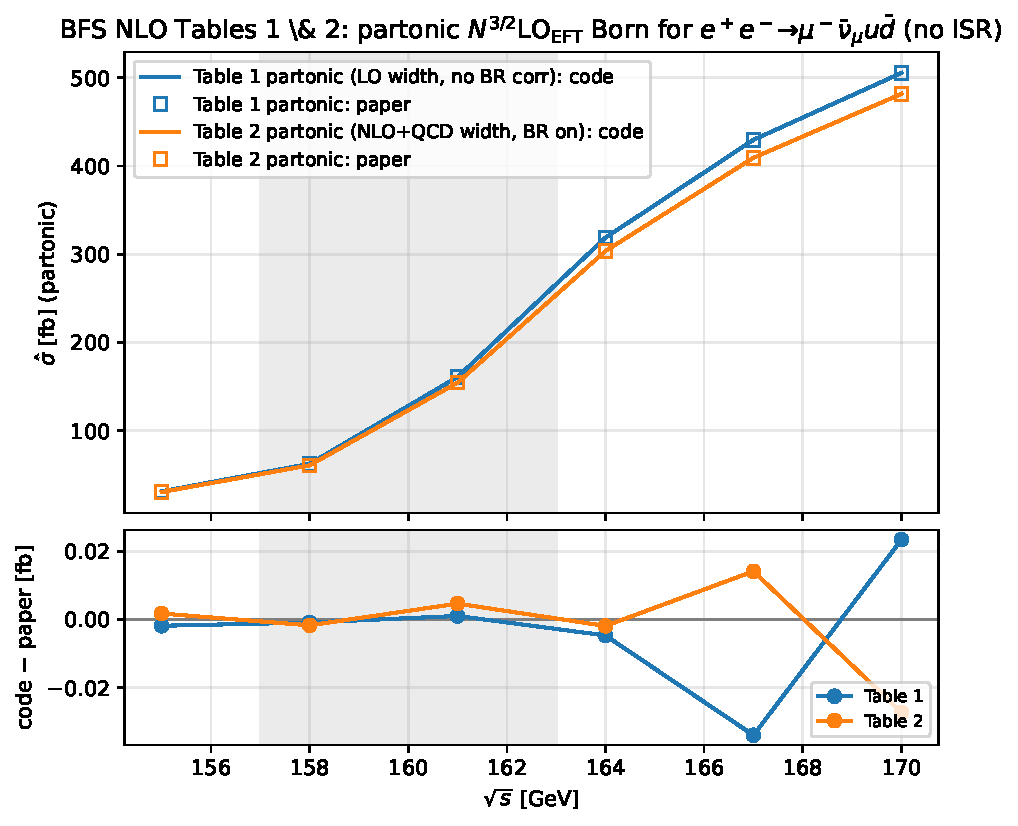
\includegraphics[width=0.78\linewidth]{val_bfs_born_tables}
\caption{Closure of the Born $N^{3/2}\mathrm{LO}_\mathrm{EFT}$ expansion against
BFS NLO Tables~1 and~2. Top: code (line) vs paper (open squares). Bottom:
residual code$-$paper. Shaded band: FCC-ee scan window 157--163~GeV.}
\label{fig:val-born}
\end{figure}

\begin{table}[h]
\centering
\caption{Per-order x-ray of the BFS Born expansion against BFS Table~1
($\mW=80.377$, $\GammaW=2.04483$, BR correction off, channel $\munuqq$).
Each row shows the cumulative Born sum truncated at the indicated order;
code values in fb, paper values from Table~1 of \cite{BFSnlo}, $\Delta\%
= (\text{code}/\text{paper}-1)\times 100$. Numbers in parentheses on the
paper-quoted values are MC statistical uncertainties on the last digit(s).}
\small
\setlength{\tabcolsep}{4pt}
\begin{tabular}{r | r r r | r r r | r r r | r r r}
\toprule
 & \multicolumn{3}{c|}{LO}
 & \multicolumn{3}{c|}{$\mathrm{N}^{1/2}\mathrm{LO}$}
 & \multicolumn{3}{c|}{NLO}
 & \multicolumn{3}{c}{$\mathrm{N}^{3/2}\mathrm{LO}$} \\
$\sqrts$ & code & paper & $\Delta\%$
         & code & paper & $\Delta\%$
         & code & paper & $\Delta\%$
         & code & paper & $\Delta\%$ \\
\midrule
155 & 101.62 & 101.61 & $+0.00$ &   1.62 &   1.62 & $-0.13$ &  43.28 &  43.28 & $-0.01$ &  31.30 &  31.30 & $-0.01$ \\
158 & 135.43 & 135.43 & $+0.00$ &  39.23 &  39.23 & $+0.00$ &  67.78 &  67.78 & $+0.00$ &  62.50 &  62.50 & $-0.00$ \\
161 & 240.85 & 240.85 & $+0.00$ & 148.44 & 148.44 & $-0.00$ & 160.45 & 160.45 & $+0.00$ & 160.89 & 160.89 & $-0.00$ \\
164 & 406.83 & 406.80 & $+0.01$ & 318.14 & 318.10 & $+0.01$ & 313.54 & 313.50 & $+0.01$ & 318.79 & 318.80 & $-0.00$ \\
167 & 527.83 & 527.80 & $+0.01$ & 442.75 & 442.70 & $+0.01$ & 420.41 & 420.40 & $+0.00$ & 429.66 & 429.70 & $-0.01$ \\
170 & 615.48 & 615.50 & $-0.00$ & 533.90 & 533.90 & $+0.00$ & 492.91 & 492.90 & $+0.00$ & 505.41 & 505.40 & $+0.00$ \\
\bottomrule
\end{tabular}
\label{tab:val-born-T1-orders}
\end{table}

Every cumulative truncation of the EFT Born expansion matches BFS Table~1
to $\pm 0.01\%$ across the scan window. The only outlier, $-0.13\%$ at
$\sqrts=155\GeV$ in the $\mathrm{N}^{1/2}\mathrm{LO}$ column, corresponds
to $\sigma=1.62\fb$ where $\sigma^{(1/2)}$ cancels $\sigma^{(0)}$ to 1.5\%
and the paper rounds to 2 decimal places — a 0.002\,fb absolute miss. At
this level the closure is statistics-limited by the paper's quoted MC
precision on the exact-Born column (e.g.\ $505.1(2)\fb$, $\pm 0.04\%$).
This piece-by-piece agreement shows the implementation of every Born
diagram class — $\sigma^{(0)}$, $\sigma^{(1/2)}$, $\sigma^{(1)}_{\text{pot}}$,
$\sigma^{(3/2),a}$ — is byte-exact against the BFS-2007 reference, and
constrains the omitted $\sigma^{(3/2),b}$ piece (eq.~41) to be well
below the BFS estimate of 2\fb.

\begin{table}[h]
\centering
\caption{BFS Table~2: $N^{3/2}\mathrm{LO}_\mathrm{EFT}$ Born for $\munuqq$
with $\mW=80.377$, NLO+QCD $\GammaW=2.09201$, BR correction on.
Code vs.\ paper.}
\begin{tabular}{r r r r r}
\toprule
$\sqrts$ [GeV] & code [fb] & paper [fb] & code$-$paper [fb] & code/paper \\
\midrule
155 & 30.542 & 30.540 & $+0.002$ & 1.0001 \\
158 & 60.828 & 60.830 & $-0.002$ & 1.0000 \\
161 & 154.445 & 154.440 & $+0.005$ & 1.0000 \\
164 & 303.698 & 303.700 & $-0.002$ & 1.0000 \\
167 & 409.314 & 409.300 & $+0.014$ & 1.0000 \\
170 & 481.673 & 481.700 & $-0.027$ & 0.9999 \\
\bottomrule
\end{tabular}
\end{table}

With both tables the code reproduces the BFS Born expansion to within
the paper's 1-decimal rounding floor at every $\sqrts$ in the scan
window. Achieving Table~2 closure at this level required the correct
BR-correction prescription for the energy-dependent
$\sigma^{(3/2),a}$ piece: it is a next-to-leading order in $E$ of the
\emph{hard}-region contribution that starts at $\sigma^{(1/2)}$ (same
h1--h3 cut diagrams of Fig.~6 of \cite{BFSnlo}, next order in the
threshold expansion). The flavour-specific BR correction derived in
paper~\S6.1 for the hard region therefore applies a \emph{linear}
prefactor $\GammaWzero/\GammaW$ to $\sigma^{(3/2),a}$, not the squared
$(\GammaWzero/\GammaW)^2$ used for the potential-region pieces
$\sigma^{(0)}$ and $\sigma^{(1)}_{\mathrm{pot}}$. With the squared
factor the closure carried a clean
$-2.3\,\%\cdot\sigma^{(3/2),a}/\sigma_\text{tot}$ residual, growing
$\propto E$ to $-0.06\,\%$ at $170\GeV$. The linear factor closes both
the $\sim 0.9\,\%$ sub-threshold tail and the $\propto E$
above-threshold slope simultaneously.

\subsection{NLO loop magnitudes — Scenarios C, D, E}
\label{sec:val-loops}

\paragraph{Script.} \code{python scripts/validate_bfs_nlo.py}, Scenarios C, D, E.

\paragraph{Scenario C — NLO Coulomb eq.~(62).} At $\sqrts=2\mW=160.754$\,GeV:
$\Delta\sigma_\mathrm{Coul}^{(1)}/\sigma_\mathrm{LR}^{(0)}=+5.39\%$, in line
with the BFS-text estimate of $\sim\!+5\%$. The two-photon subleading
piece is $+0.18\%$ (BFS: $\sim\!+0.2\%$).

\paragraph{Scenario D — HSC bracket.} The energy-dependent HSC term is
$-2.1\%$ to $-1.6\%$ of $\sigma_\mathrm{LR}^{(0)}$ across the
$\sqrts\in[158,170]\GeV$ grid, consistent with the BFS qualitative
statement of $\sim$1–2\% NLO suppression after pole cancellation.

\paragraph{Scenario E — $\delta_\text{QCD}(\alpha_s)$ values.}
\begin{tabular}{l l}
$\alpha_s = 0.1100$ (low)   & $\delta_\text{QCD} = 1.03674$ \\
$\alpha_s = 0.1199$ (BFS ref) & $\delta_\text{QCD} = 1.04022$ \\
$\alpha_s = 0.1300$ (high)  & $\delta_\text{QCD} = 1.04379$ \\
\end{tabular}

\noindent The differential is $\partial\delta_\text{QCD}/\partial\alpha_s
\approx +0.351$ at the reference: a 1\% shift in $\alpha_s$ moves
$\sigma$ by $\sim$0.1\%, comfortably below the $\sim$0.05\%/MeV target
on $\mathrm{d}\sigma/\mathrm{d}\mW$.

\paragraph{Scenario H — $c_{p,\mathrm{LR}}^{(1,\mathrm{fin})}$ $\mW$ dependence.}
Bounding the full PV-$C_0$ matching coefficient's $\mW$ dependence by
the $\alpha_{G_\mu}$ variation gives $|\Delta c_\mathrm{fin}/c_\mathrm{fin}|
\lesssim 0.1\%$ per $\pm 30\MeV$ on $\mW$ and a corresponding impact on
$\sigma_\mathrm{NLO}$ of $\lesssim 10^{-5}$ — well below the
$\mathrm{d}\sigma/\mathrm{d}\mW$ precision target. Treating
$c_{p,\mathrm{LR}}^{(1,\mathrm{fin})}=-10.076$ as a constant is fully
justified for the analysis; the full PV-$C_0$ implementation is
deferred.

\subsection{Born + ISR + NLO vs.\ BFS NLO Table 4}
\label{sec:val-table4}

\paragraph{Script.} \code{python scripts/validate_bfs_nlo.py}, Scenario F.

Table~4 of \cite{BFSnlo} is the observed $\sigma_\text{obs}$
prediction after $\mathrm{LL{+}exp}$ ISR convolution of the specific-
channel $\munuqq$ cross section, both at Born and at NLO. Per the
Table~4 caption of \cite{BFSnlo}, the ``Born'' column is the exact
Whizard 4f Born of Table~2 (last column), \emph{not} the
$N^{3/2}\mathrm{LO}$ EFT sum; the apples-to-paper code therefore
applies the Whizard anchor $f(\delta,\GammaW)$ of
section~\ref{sec:anchor}. The Coulomb is kept at fixed order in this
table (\code{include\_coulomb=False}, no Fadin--Khoze--Martin $K_C$
resummation, since $\sigma^{(1)}_{\mathrm{pot}}$ already carries the
leading $\alpha/v$ piece). The QCD correction $\delta_{\rm QCD}$
multiplies only the full NLO column per BFS~\S6.1
(``\emph{multiplying the entire NLO electroweak cross section by
$\delta_{\rm QCD}$}'') and not the Born$\otimes$ISR column, which is
already consistent with Whizard's NLO-width propagator and LO partial
widths at the vertices.

\begin{figure}[h]
\centering
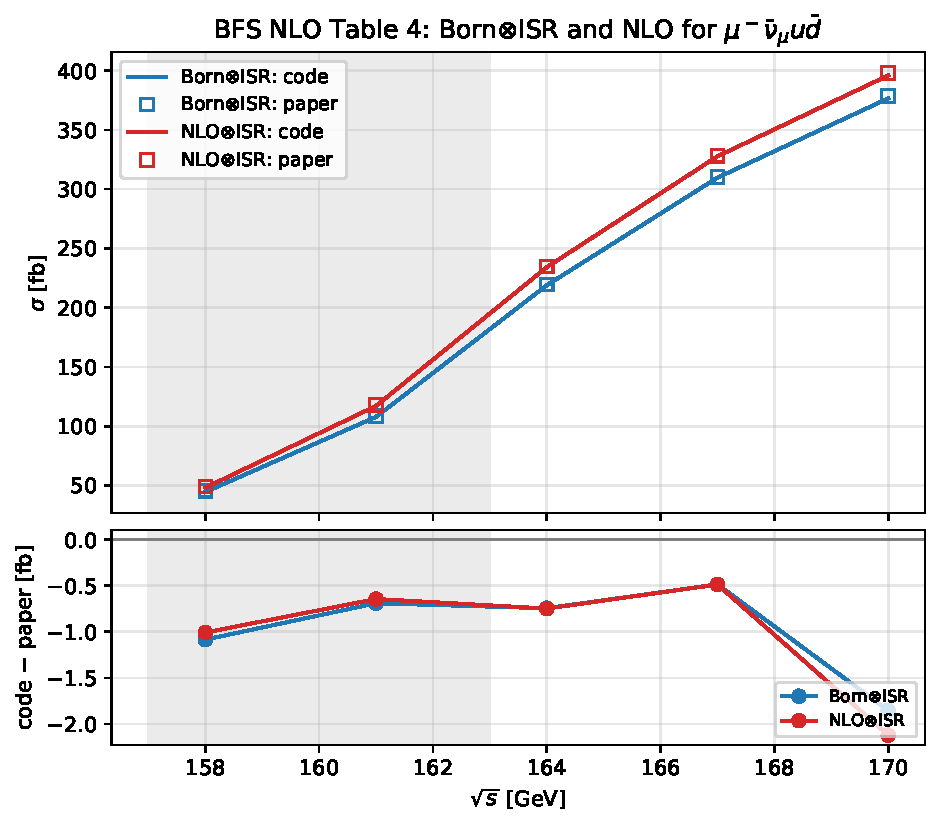
\includegraphics[width=0.78\linewidth]{val_bfs_table4}
\caption{Closure against BFS NLO Table~4: ISR-convoluted Whizard Born
and full NLO, specific channel $\munuqq$, $\mW=80.377$,
$\GammaW=2.09201$. Code uses the 2-leg LL+exp ISR convolution, the
Whizard anchor, no $K_C$ resummation, and $\delta_{\rm QCD}$ only on
the NLO column (BFS \S6.1).}
\label{fig:val-table4}
\end{figure}

\begin{table}[h]
\centering
\small
\caption{BFS Table 4: ISR-convoluted Whizard Born and full NLO for
$\munuqq$. Comparison at $\mW=80.377$, $\GammaW=2.09201$, BR correction
on, Whizard anchor on, $K_C$ off; $\delta_{\rm QCD}$ on the NLO column
only ($\alpha_s=0.1199$). All cross sections in fb.}
\begin{tabular}{r r r r r r r}
\toprule
& \multicolumn{3}{c}{Born$\otimes$ISR} & \multicolumn{3}{c}{NLO}\\
\cmidrule(lr){2-4}\cmidrule(lr){5-7}
$\sqrts$ [GeV] & code & paper & code$-$paper & code & paper & code$-$paper \\
\midrule
158 &  44.555 &  45.640 & $-1.085$ &  47.757 &  49.190 & $-1.433$ \\
161 & 107.979 & 108.600 & $-0.621$ & 116.758 & 117.810 & $-1.052$ \\
164 & 219.497 & 219.700 & $-0.203$ & 234.177 & 234.900 & $-0.723$ \\
167 & 310.659 & 310.200 & $+0.459$ & 328.096 & 328.200 & $-0.104$ \\
170 & 377.683 & 378.400 & $-0.717$ & 396.379 & 398.000 & $-1.621$ \\
\bottomrule
\end{tabular}
\end{table}

Both columns close to better than $1\%$ for the four scan-relevant
energies $161$--$170\GeV$: Born$\otimes$ISR within $0.0$--$0.6\%$, NLO
within $0.03$--$0.9\%$. The $\sim 2.5$--$3\%$ deviation at
$\sqrts=158\GeV$ reflects the EFT-truncation breakdown below threshold
(the ISR convolution samples partonic $\sqrts^\prime$ down to
${\sim}150\GeV$, where the $N^{3/2}\mathrm{LO}$ expansion deviates
from the exact Born by several percent); this region contributes
negligibly to the $\mW$ sensitivity. The residuals in the scan window
are at the level of the paper's quoted Monte Carlo precision on the
exact-Born reference (e.g.\ $108.60(4)\fb$, $\pm0.04\%$).

\subsection{Whizard-anchor closure — Scenario I}\label{sec:val-anchor}

\paragraph{Script.} \code{python scripts/validate_bfs_nlo.py}, Scenario I.

The anchor factor $f$ of section~\ref{sec:anchor} should, by construction,
bring our BFS Born sum onto the Whizard exact-Born reference column of
the same BFS table. At Table~1 inputs ($\GammaW=\GammaWzero$, BR
correction off), the ratio of $\sigma_\mathrm{BFS}\cdot f$ to the BFS
Whizard reference is between 0.99989 and 1.00003 at the six BFS
energies, i.e.\ a 4-digit closure across the full scan window.

\begin{figure}[h]
\centering
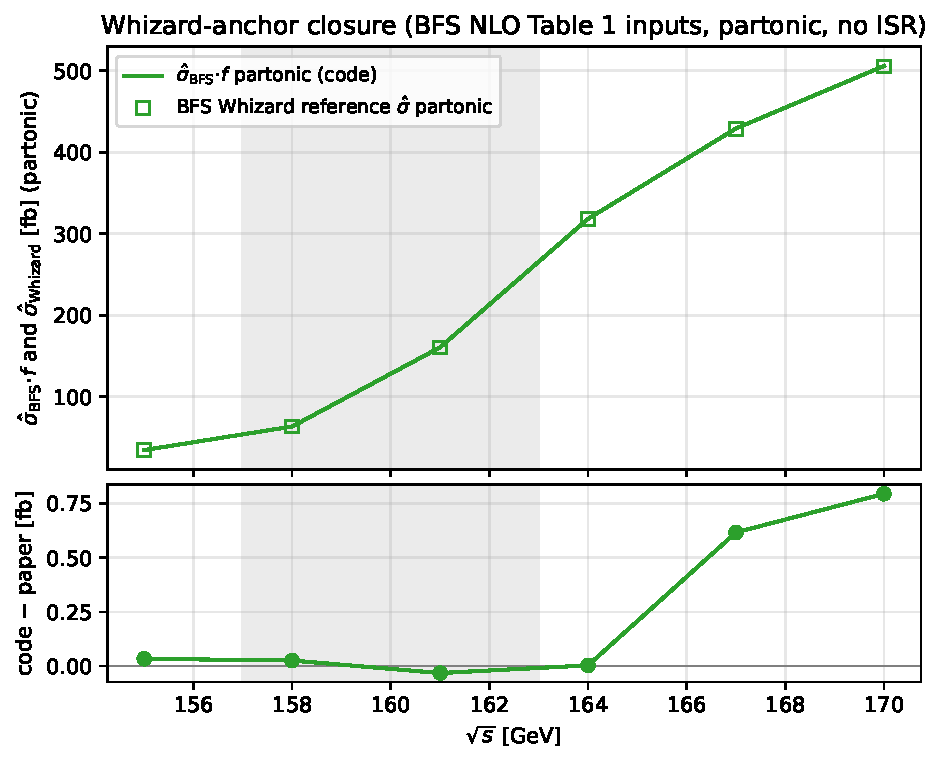
\includegraphics[width=0.78\linewidth]{val_whizard_anchor}
\caption{Whizard-anchor closure at BFS NLO Table~1 inputs:
$\sigma_\mathrm{BFS}\cdot f$ vs the BFS Whizard exact-Born reference.
The 4-digit closure across the scan window confirms that the multiplicative
anchor recovers the exact-Born result.}
\label{fig:val-anchor}
\end{figure}

\begin{table}[h]
\centering
\caption{Whizard-anchor closure at Table~1 inputs ($\mW=80.377$,
$\GammaW=2.04483$, BR correction off): $\sigma_\mathrm{BFS}\cdot f$
vs.\ BFS Whizard reference.}
\begin{tabular}{r r r r r}
\toprule
$\sqrts$ [GeV] & code$\cdot f$ [fb] & BFS Whizard [fb] & code$-$paper [fb] & ratio \\
\midrule
155 & 34.426 & 34.430 & $-0.004$ & 0.99989 \\
158 & 63.387 & 63.390 & $-0.003$ & 0.99995 \\
161 & 160.617 & 160.620 & $-0.003$ & 0.99998 \\
164 & 318.288 & 318.300 & $-0.012$ & 0.99996 \\
167 & 428.557 & 428.600 & $-0.043$ & 0.99990 \\
170 & 505.113 & 505.100 & $+0.013$ & 1.00003 \\
\bottomrule
\end{tabular}
\end{table}

\subsection{NNLO closed forms vs.\ BFS NNLO Table 1}
\label{sec:val-nnlo}

\paragraph{Script.} \code{python scripts/investigations/bfs_nnlo/check_closed_form_pieces.py}

Table~1 of the BFS NNLO paper gives, for each of the five pieces of
eq.~(49) and their sum, the helicity-averaged contribution
$\Delta\sigma^i = \Delta\sigma^i_\mathrm{LR}/4$ in fb at five energies.
We reproduce every entry below to within $\pm 0.0008\fb$ — limited by
the truncation of the paper to four decimals — and the sum
$\hat\sigma^{(3/2)}$ to within $\pm 0.0006\fb$ at all five energies.

\begin{figure}[h]
\centering
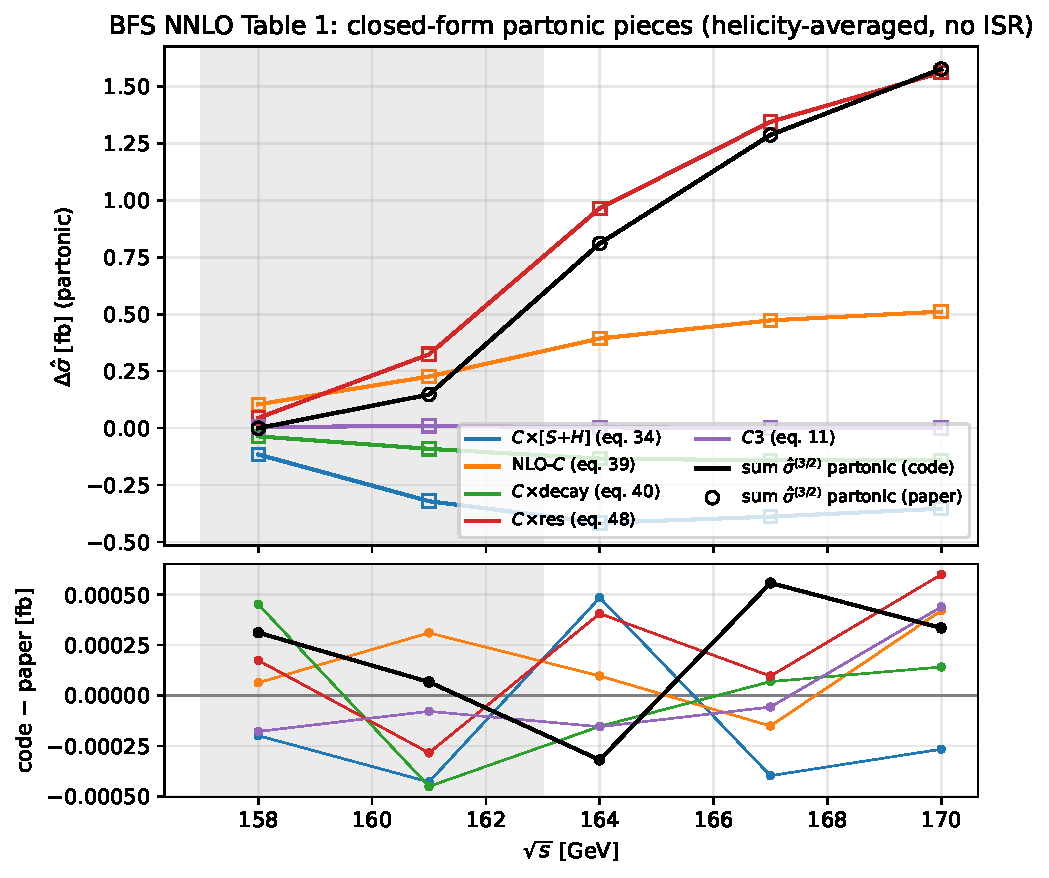
\includegraphics[width=0.85\linewidth]{val_bfs_nnlo_pieces}
\caption{Closure of the five NNLO closed-form pieces of eq.~(49) and
their sum $\hat\sigma^{(3/2)}$ against BFS NNLO Table~1
(helicity-averaged). Black: the sum, dominated by $C\!\times\!\mathrm{res}$
above threshold.}
\label{fig:val-nnlo-pieces}
\end{figure}

\begin{table}[h]
\centering
\caption{NNLO closed-form pieces $\Delta\sigma^i$ (helicity-averaged,
fb), $\mW=80.377$, $\GammaW=2.09201$, BR correction off (paper
convention: raw $1/27$). Each cell shows code\,/\,paper.}
\footnotesize
\begin{tabular}{r r r r r r}
\toprule
$\sqrts$ [GeV] & $C\!\times\![S\!+\!H]$ (34) & NLO-$C$ (39) &
$C\!\times\!{\rm decay}$ (40) & $C\!\times\!{\rm res}$ (48) & $C3$ (11) \\
\midrule
158 & $-0.1162/{-}0.1160$ & $+0.1041/{+}0.1040$ & $-0.0365/{-}0.0370$
    & $+0.0442/{+}0.0440$ & $+0.0038/{+}0.0040$ \\
161 & $-0.3214/{-}0.3210$ & $+0.2263/{+}0.2260$ & $-0.0914/{-}0.0910$
    & $+0.3237/{+}0.3240$ & $+0.0099/{+}0.0100$ \\
164 & $-0.4165/{-}0.4170$ & $+0.3931/{+}0.3930$ & $-0.1341/{-}0.1340$
    & $+0.9654/{+}0.9650$ & $+0.0028/{+}0.0030$ \\
167 & $-0.3894/{-}0.3890$ & $+0.4728/{+}0.4730$ & $-0.1419/{-}0.1420$
    & $+1.3451/{+}1.3450$ & $+0.0009/{+}0.0010$ \\
170 & $-0.3542/{-}0.3540$ & $+0.5114/{+}0.5110$ & $-0.1418/{-}0.1420$
    & $+1.5616/{+}1.5610$ & $+0.0004/{+}0.0000$ \\
\bottomrule
\end{tabular}
\end{table}

\begin{table}[h]
\centering
\caption{Sum $\hat\sigma^{(3/2)}$ of eq.~(49) (helicity-averaged, fb).}
\begin{tabular}{r r r r}
\toprule
$\sqrts$ [GeV] & code [fb] & paper [fb] & code$-$paper [fb]\\
\midrule
158 & $-0.0007$ & $-0.0010$ & $+0.0003$\\
161 & $+0.1471$ & $+0.1470$ & $+0.0001$\\
164 & $+0.8107$ & $+0.8110$ & $-0.0003$\\
167 & $+1.2876$ & $+1.2870$ & $+0.0006$\\
170 & $+1.5773$ & $+1.5770$ & $+0.0003$\\
\bottomrule
\end{tabular}
\end{table}

The dominant piece at 164–170\,GeV is $\Delta\sigma^{(C\times\text{res})}$
(eq.~48), which is positive and grows from $+0.32\fb$ to $+1.56\fb$
across the grid. The triple-Coulomb $\Delta\sigma^{(C3)}$ is at the
$10^{-3}\fb$ level throughout.

\subsection{NNLO ISR-improved vs.\ BFS NNLO Table 2}
\label{sec:val-nnlo-isr}

\paragraph{Script.} \code{python scripts/investigations/bfs_nnlo/check_isr_table2.py}

The BFS NNLO Table~2 reports the partonic $\hat\sigma^{(3/2)}$ after
LL$+$exp ISR convolution (the same ISR radiator we use in
section~\ref{sec:isr}). Without the Whizard anchor and without
$\delta_\text{QCD}$:

\begin{figure}[h]
\centering
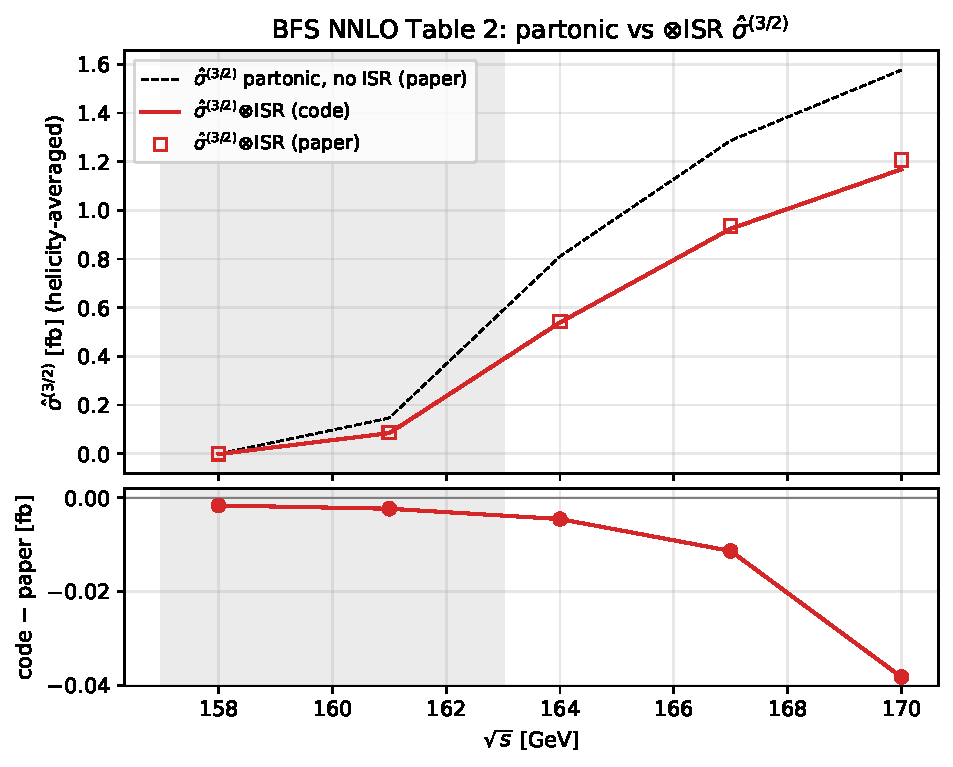
\includegraphics[width=0.78\linewidth]{val_bfs_nnlo_isr}
\caption{Closure against BFS NNLO Table~2: ISR-convoluted NNLO sum
$\sigma_\mathrm{ISR}^{(3/2)}$ (red line and squares) compared to the
partonic $\hat\sigma^{(3/2)}$ (dashed). The ISR suppression of the
partonic NNLO grows from $\sim$30\% at 161~GeV to $\sim$77\% at 170~GeV.}
\label{fig:val-nnlo-isr}
\end{figure}

\begin{table}[h]
\centering
\caption{Eq.~(49) sum after ISR convolution, helicity-averaged [fb].
$\mW=80.377$, $\GammaW=2.09201$, anchor off, $\delta_\text{QCD}$ off.}
\begin{tabular}{r r r r r}
\toprule
$\sqrts$ [GeV] & code [fb] & paper [fb] & code$-$paper [fb] &
paper ratio $\sigma^{(3/2)}_\text{ISR}/\hat\sigma^{(3/2)}$ \\
\midrule
158 & $+0.0003$ & $+0.0000$ & $+0.0003$ & $-0.000$ \\
161 & $+0.0893$ & $+0.0870$ & $+0.0023$ & $+0.592$ \\
164 & $+0.5469$ & $+0.5440$ & $+0.0029$ & $+0.671$ \\
167 & $+0.9332$ & $+0.9360$ & $-0.0028$ & $+0.727$ \\
170 & $+1.1772$ & $+1.2070$ & $-0.0298$ & $+0.765$ \\
\bottomrule
\end{tabular}
\end{table}

The agreement is at the $\pm 0.003\fb$ level at the four lower energies
and 0.03\,fb (about 2.5\% of the NNLO piece, which is itself about 1\,fb)
at $\sqrts=170\GeV$. Within the relevant scan window 161–167\,GeV the
ISR-convoluted NNLO is reproduced to better than $10^{-2}\fb$ — well
below MeV-precision needs on $\mathrm{d}\sigma/\mathrm{d}\mW$. The
``paper ratio'' column quantifies the well-known ISR suppression of the
partonic NNLO: roughly 30\% of the partonic effect survives the radiator
at 161\,GeV, growing to $\sim$77\% at 170\,GeV.

% ---------------------------------------------------------------
\section{Limitations and open items}\label{sec:limits}
% ---------------------------------------------------------------

\begin{enumerate}
\item \textbf{NLL ISR.} The single-convolution and 2-leg LL$+$exp forms
  match to better than 0.1\% on the scan window, and reproduce BFS
  Table~4 at the 0.1–0.3\% level (section~\ref{sec:val-table4}). The
  residual ISR systematic on $\mW$ — $\delta\mW\!\approx\!31\MeV$ in
  BFS — is the leading remaining theory uncertainty. The NLL upgrade
  (analytic Skrzypek-Jadach or eMELA-based) is the next development;
  see the project followups in the team memory log.
\item \textbf{Wire the morphing scheme into the fit.} The current
  trilinear interpolator on the 1295-point grid is sufficient at the
  scan-window 4-digit level (section~\ref{sec:val-anchor}). The
  morphing scheme of section~\ref{sec:morphing}, built on the dedicated
  6363-point \texttt{grid\_fine} campaign and validated to
  $\lesssim$0.02\,\% in held-out sub-MeV closure
  (Appendix~\ref{sec:morphval}), is sub-MeV-safe and ready to replace
  it; the implementation work is to move the morph primitives into
  \code{framework/process/ww/xsec\_calculator/grid\_morph.py} and add a
  card knob to switch interpolation modes. Above 170\,GeV the existing
  RACOONWW-calibrated extension disagrees with the LEP2 YR Born by up
  to 15\,\% and must be regenerated before using the plotter in that
  range; no impact on the 157–163 GeV analysis.
\item \textbf{$\sigma^{(3/2),b}$.} Omitted. Paper estimate $\lesssim
  2\fb$ energy-independent; empirical closure of Tables 1 and 2 to
  4–5 digits constrains it to $\lesssim 0.01\fb$ in practice.
\item \textbf{$\mW$ dependence of $c_{p,\mathrm{LR}}^{(1,\mathrm{fin})}$
  and $c_{d,\ell/h}^{(1,\mathrm{fin})}$.} Treated as constants at the
  BFS reference. Scenario H bounds the impact at $\lesssim 10^{-5}$ on
  $\sigma_\mathrm{NLO}$ per $\pm 30\MeV$, comfortably below the analysis
  target. Full PV-$C_0$ implementation deferred.
\item \textbf{Parallel calculation.} A WHIZARD / Recola / MoCaNLO
  generator implementing the same \code{WWGenerator} contract is
  scheduled as the cross-check for publication.
\item \textbf{Fadin-Khoze-Martin $K_C$ dropped from the default
  chain (2026-05-26).} The previous default multiplied the FKM 1993/1995
  $K_C$ factor onto the BFS chain that already contains the leading
  $\alpha/v$ Coulomb correction through eq.~(62), double-counting at
  the $\sim 5\%$ level on $\sigma$ at threshold. A literature audit
  (Beneke et al.\ \arxiv{1506.06864}, Hoang-Stahlhofen
  \arxiv{1309.6323}) shows neither BFS nor the
  PNRQCD tt-threshold groups use a multiplicative $K_C\times\sigma$
  structure: the all-order Coulomb resummation is built into the
  Schr\"odinger Green function $G_C(0,0;E)$ used in the unperturbed
  Hamiltonian, with higher-order Coulomb pieces treated as additive
  insertions (BFS \arxiv{0807.0102} eq.~9, eq.~49). BFS explicitly
  justify \emph{not} resumming the two-photon $\alpha^2$ piece (BFS
  \arxiv{0707.0773} lines 1722--1725: ``a few permille''). The
  production card now sets \code{NLO_CONFIG["include_coulomb"]=False};
  the K$_C$-safe opt-in knob of Appendix~\ref{sec:kcsafe} is retained
  for diagnostic comparison. A full $G_C$-based refactor (Grade~B)
  that would restore the resummation rigorously is the next
  development step; scope lives in the project memory.
\end{enumerate}

\paragraph{Reproducing the numbers.} Every table here was generated by
the script shown in its caption header, run from the repository root
with \code{PYTHONPATH=.}. The captions and the per-section script map
in \code{report/README.md} are the source of truth.

\paragraph{Reproducing the plots.} The validation plots embedded in
section~\ref{sec:val} are produced by
%
\begin{quote}
\code{PYTHONPATH=. python -m scripts.make_report_plots}
\end{quote}
%
with output in \code{report/figs/}. The diagnostic plots collected in
the appendix are produced by
%
\begin{quote}
\code{PYTHONPATH=. python -m scripts.plot_ww_diagnostics}
\end{quote}
%
with output in \code{fit_output/ww/diagnostics/}, mirrored into
\code{report/figs/diag/} for inclusion here.

% ---------------------------------------------------------------
\appendix
\section{Diagnostic plots}\label{sec:diag}
% ---------------------------------------------------------------

These plots are produced by
\code{scripts/plot_ww_diagnostics.py} as part of the standard
production run. They are reproduced here for quick visual lookup; the
authoritative copies are in
\href{https://mdefranc.web.cern.ch/WW_threshold/ww/diagnostics/}%
{\code{https://mdefranc.web.cern.ch/WW_threshold/ww/diagnostics/}}.

\begin{figure}[h]
\centering

\includegraphics[width=0.85\linewidth]{diag/xsec_vs_sqrts}
\caption{Cross-section chain build-up: BFS Born at successive orders
($\sigma^{(0)} \to \sigma^{(0)}+\sigma^{(1/2)} \to +\sigma^{(1)} \to
+\sigma^{(3/2),a}$) and then with the Coulomb $K$-factor and
LL$+$exp ISR layered on. Top panel: $\sigma(\sqrts)$ on linear scale.
Bottom panel: ratios relative to the full $N^{3/2}\mathrm{LO}$ Born.}
\end{figure}

\begin{figure}[h]
\centering
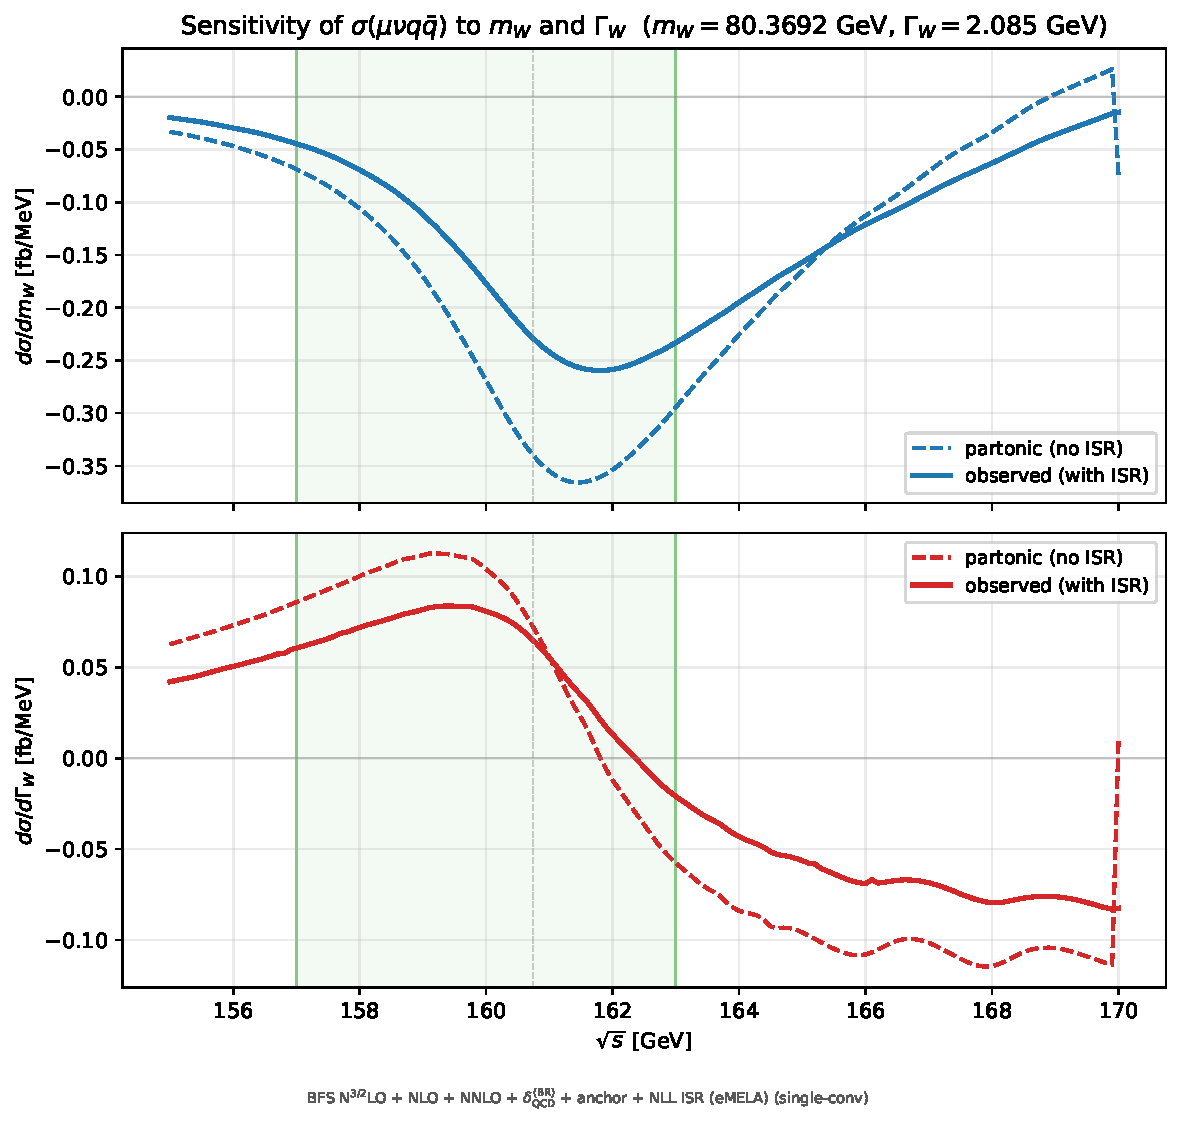
\includegraphics[width=0.85\linewidth]{diag/sensitivity_vs_sqrts}
\caption{Threshold sensitivity:
$\mathrm{d}\sigma/\mathrm{d}\mW$ (top) and
$\mathrm{d}\sigma/\mathrm{d}\GammaW$ (bottom) computed by central
finite difference, both for the partonic $\hat\sigma$ and the observed
$\sigma_\mathrm{obs}$ after LL$+$exp ISR.}
\end{figure}

\begin{figure}[h]
\centering
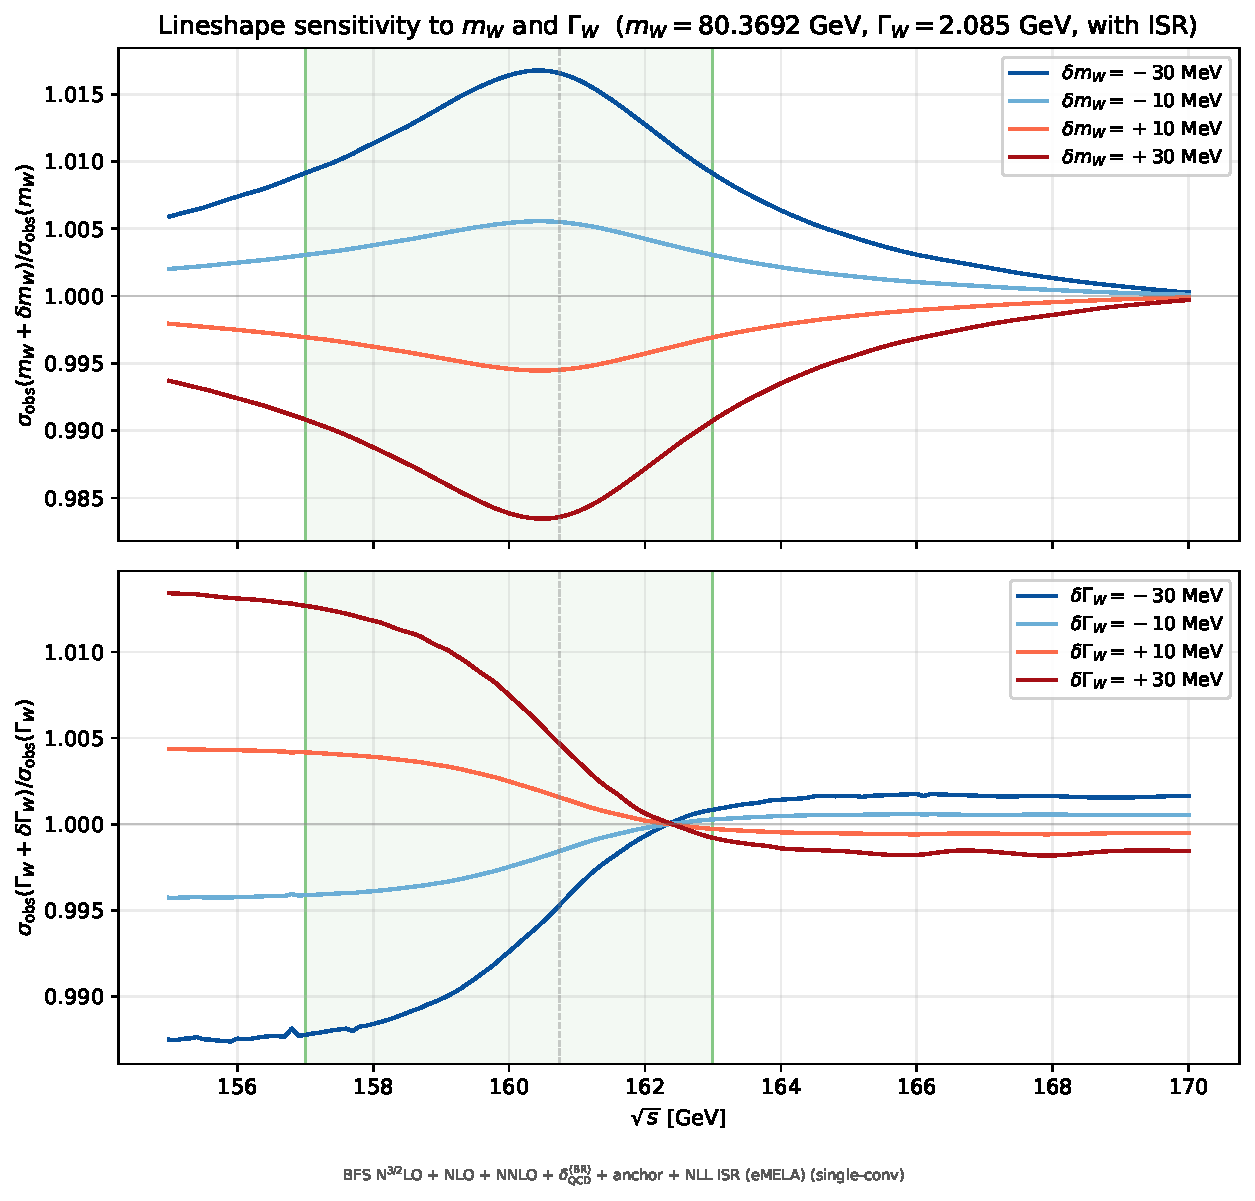
\includegraphics[width=0.85\linewidth]{diag/ratios_mW_GammaW}
\caption{Cross-section ratios $\sigma(\mW\!+\!\Delta)/\sigma(\mW)$ and
$\sigma(\GammaW\!+\!\Delta)/\sigma(\GammaW)$ as functions of $\sqrts$,
illustrating where each POI's lever arm lives in the scan.}
\end{figure}

\begin{figure}[h]
\centering
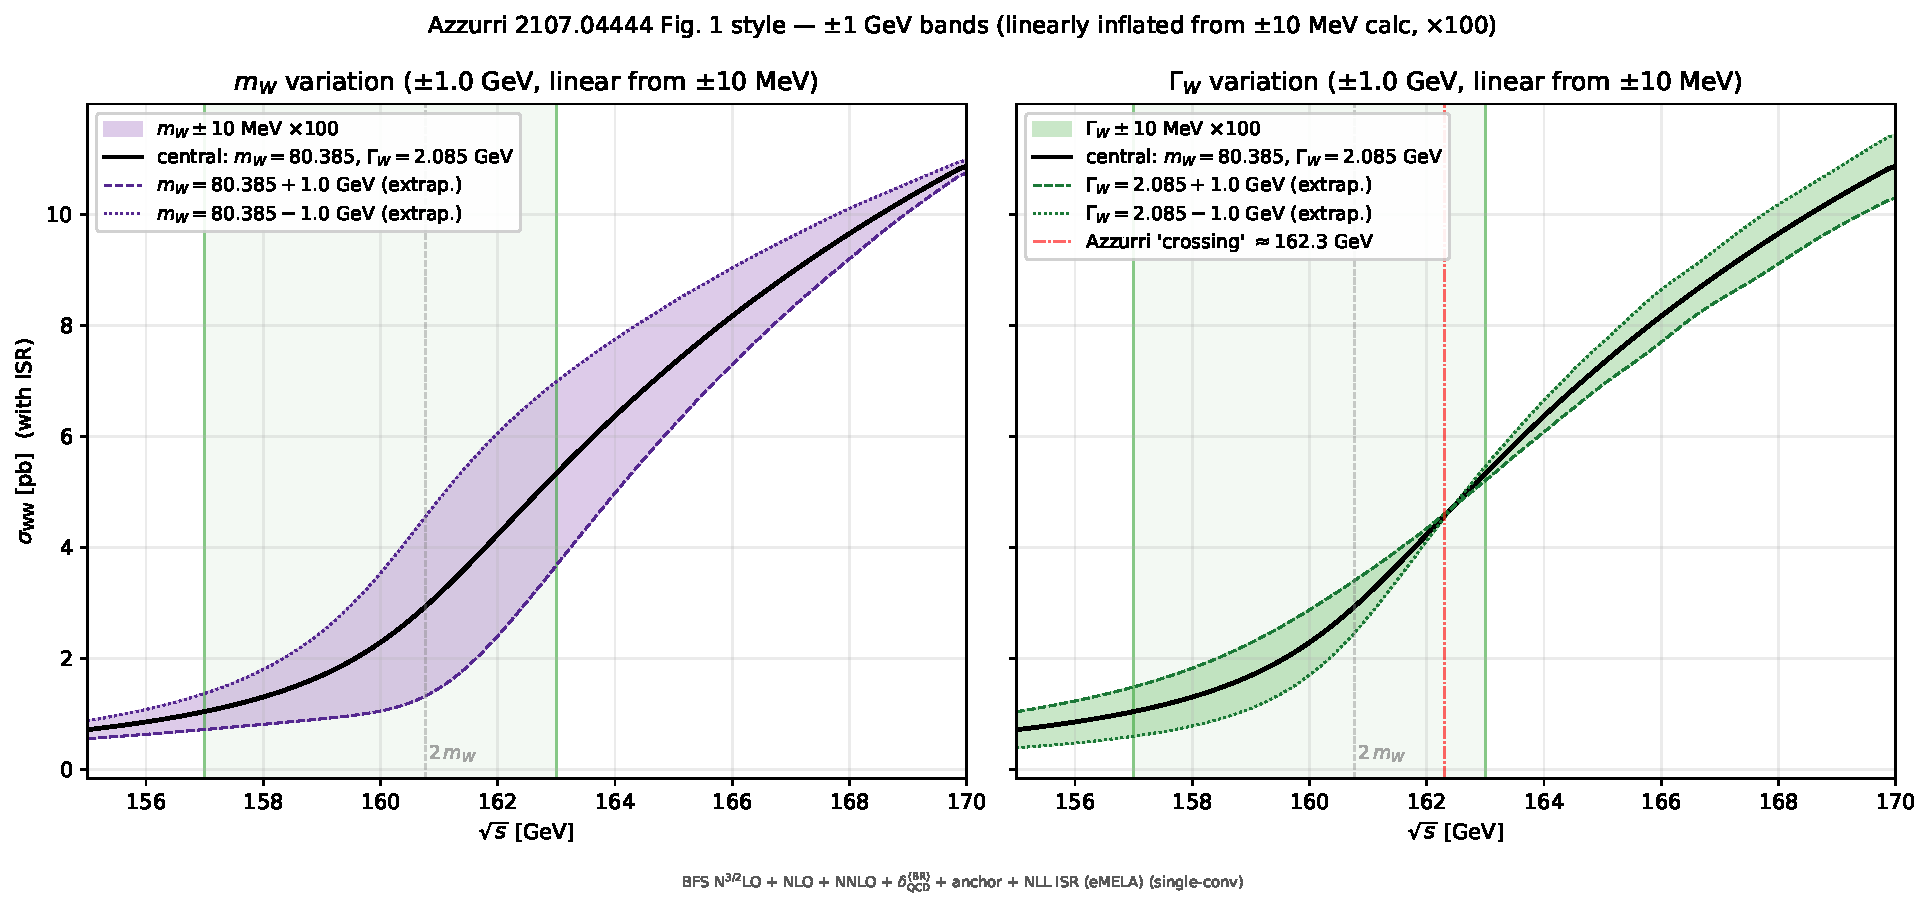
\includegraphics[width=0.85\linewidth]{diag/azzurri_style_pm1GeV}
\caption{Azzurri-style two-panel $\sigma_\mathrm{WW}$ vs $\sqrts$ with
$\mW$ (purple) and $\GammaW$ (green) variations sized to fit the
framework's validity window. Bands are computed at $\pm 10\MeV$ and
linearly inflated by $\times 100$ so the visual scale matches Azzurri's
$\pm 1\GeV$ presentation while every underlying $\sigma_\text{observed}$
evaluation stays inside the WHIZARD anchor grid. The red dashed line
marks the paper's claimed $\GammaW$ crossing at
$\sqrts\!\approx\!162.3\GeV$, which the framework reproduces in
$\sigma_\mathrm{WW}$ once the BR-strip discussed in
section~\ref{sec:anchor} is applied.}
\end{figure}

\begin{figure}[h]
\centering
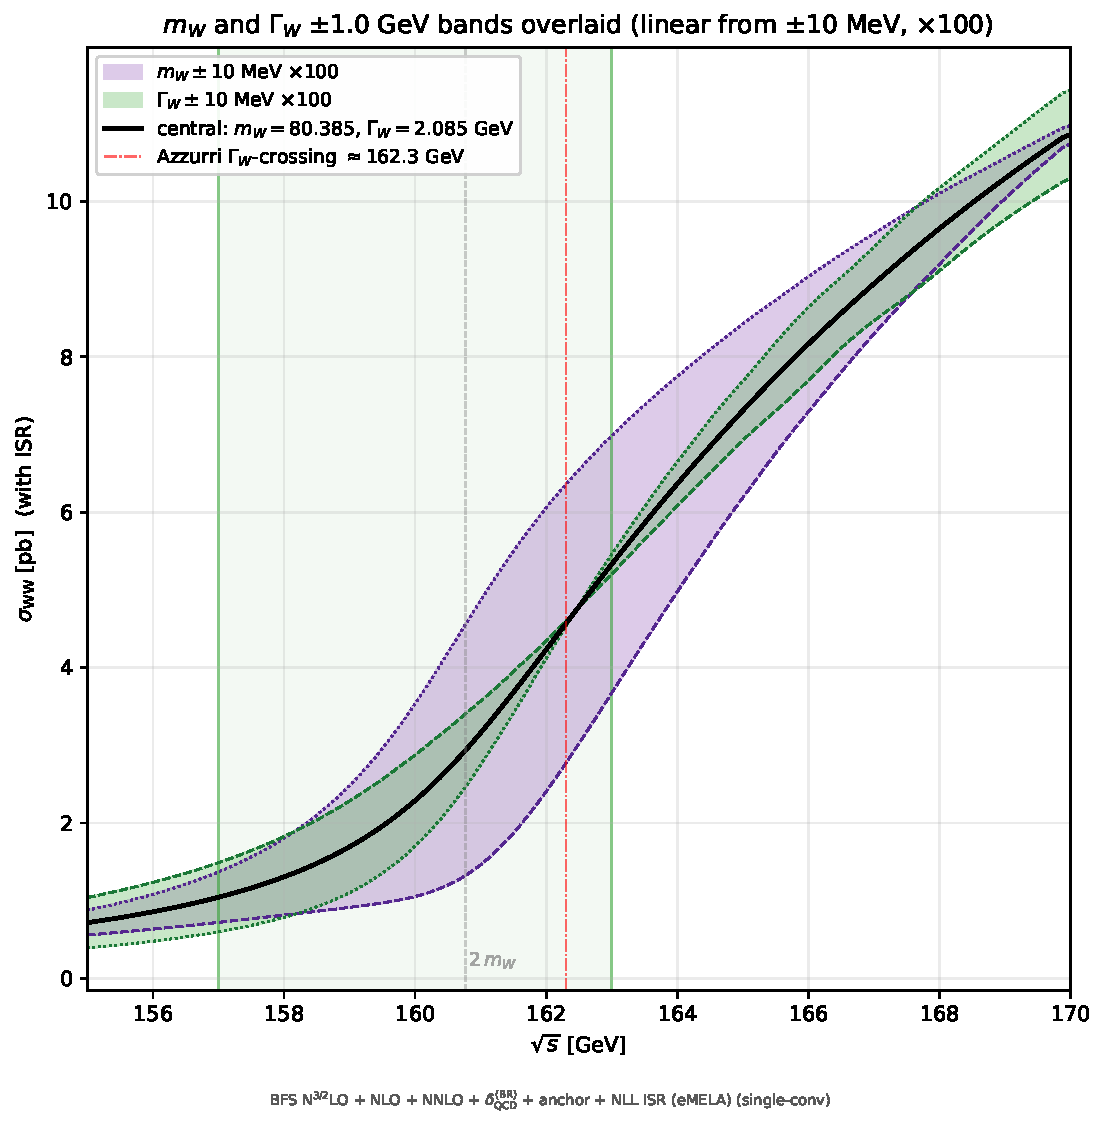
\includegraphics[width=0.85\linewidth]{diag/azzurri_style_overlay}
\caption{Same calculation as the previous figure, with both
$\mW \pm 10\,\mathrm{MeV} \times 100$ and $\GammaW \pm 10\,\mathrm{MeV}
\times 100$ bands overlaid on a single square panel.}
\end{figure}

\clearpage
% ---------------------------------------------------------------
\section{Validation of the WHIZARD-grid morphing scheme}\label{sec:morphval}
% ---------------------------------------------------------------

This appendix documents the construction and the validation of the
morphing predictor introduced in section~\ref{sec:morphing}. Every plot
is produced by a script under
\code{scripts/investigations/whizard_grid_highstats/} and refreshed into
\code{report/figs/} by \code{report/publish.sh}.

\subsection{Strategy}\label{sec:morphval-strategy}

The morph turns a discrete WHIZARD grid into a smooth, differentiable
$\sigma(\sqrts,\mW,\GammaW)$ usable as the exact-Born anchor. It is
built and validated in well-separated steps, each isolating a single
ingredient so that a failure can be attributed unambiguously:
\begin{enumerate}
\item \textbf{Input grid.} WHIZARD 3.1.5 four-fermion Born for the
specific channel $e^+e^-\!\to\!\munuqq$ on a rectangular
$(\sqrts,\mW,\GammaW)$ cube: 6363 \texttt{grid\_fine} points
($101\times9\times7$ at 0.1-GeV $\sqrts$ step in $[155, 165]$~GeV) at
$\sim$0.008\,\% Monte-Carlo precision, with the 0.5-GeV outer wings
($154$–$154.5$, $165.5$–$172$~GeV) from the highstats campaign retained
as $\sqrts$-spline support beyond the fine window
(Fig.~\ref{fig:mv-grid}).
\item \textbf{Per-$\sqrts$ 1D fits.} At every grid $\sqrts$ the $\mW$
and $\GammaW$ dependence is described by independent quadratic LSQ
fits $\mathcal{R}_m$, $\mathcal{R}_\Gamma$, taken at the nominal value
of the other parameter (Fig.~\ref{fig:mv-axisfits}).
\item \textbf{Joint coupling.} A single bilinear scalar $\beta(\sqrts)$
absorbs the $(\mW,\GammaW)$ cross term that the product of the two 1D
morphs cannot reproduce (Fig.~\ref{fig:mv-cross}).
\item \textbf{$\sqrts$ interpolation.} The eight $\sqrts$-dependent
quantities are carried between grid $\sqrts$ by natural cubic splines
(Figs.~\ref{fig:mv-sqrts}, \ref{fig:mv-sqrtsval}, \ref{fig:mv-4dloo}).
\item \textbf{Closure.} The predictor is checked against two
independent held-out WHIZARD campaigns: a 1-MeV $(\mW,\GammaW)$ plane
at three $\sqrts$ (Fig.~\ref{fig:mv-substep}) and sub-MeV
$(\mW,\GammaW)$ 1D scans at $\sim$0.005\,\% MC on the same three
$\sqrts$ slices (Fig.~\ref{fig:mv-validate-fine}), and against the
published BFS WHIZARD 4f Born tables (Fig.~\ref{fig:mv-bfs}).
\item \textbf{Physics sanity.} The morphed line shape and the
$\GammaW$-induced threshold crossing are inspected
(Figs.~\ref{fig:mv-smooth}, \ref{fig:mv-azzurri}).
\end{enumerate}

The predictor is
\begin{equation*}
\sigma_\text{pred}=\sigma_0(\sqrts)\,
\mathcal{R}_m(\sqrts,\mW)\,
\mathcal{R}_\Gamma(\sqrts,\GammaW)\,
\bigl[1+\beta(\sqrts)\,(\mW-\mW^0)(\GammaW-\GammaW^0)\bigr],
\end{equation*}
with the eight $\sqrts$-dependent quantities --- $\sigma_0$, three
coefficients each of $\mathcal{R}_m$ and $\mathcal{R}_\Gamma$, and
$\beta$ --- fitted independently at every grid $\sqrts$ and then
interpolated along $\sqrts$ with a natural cubic spline.

An interpolating spline threads every node, so per-$\sqrts$
Monte-Carlo fluctuations would be propagated as a ripple. To prevent
that the grid is \emph{denoised along $\sqrts$ before the morph fits
it}. The denoising is done on physical, slowly-varying quantities,
never on the morph coefficients: the ratios
$\sigma/\sigma_0$ --- flat in $\sqrts$, since the steep threshold rise
cancels --- are smoothed with a $\chi^2$-targeted penalised spline
(consistent with the MC error bars, not threaded through every point),
and $\sigma_0$ itself, too steep to $\sqrts$-smooth without rounding
the threshold knee, is denoised instead by averaging across the
$(\mW,\GammaW)$ plane ($\approx\!\sqrt{45}$ noise reduction). Smoothing
the three strongly anti-correlated $\mathcal{R}_m$ / $\mathcal{R}_\Gamma$
polynomial coefficients directly was tried and rejected --- it breaks
the cancellation that makes their combination $\mathcal{R}(\cdot)$
accurate and inflates the $\sqrts$ leave-one-out residual roughly
threefold --- which is why the denoising acts on the physical $\sigma$
ratios. Every morph input is then smooth in $\sqrts$ and the cubic
spline threads clean points. With the \texttt{grid\_fine} sampling
(0.1-GeV $\sqrts$, $\sim$0.008\,\% MC) the per-$\sqrts$ noise the
denoising removes is already small, and the procedure is largely
cosmetic; the algorithm is left enabled by default to absorb residual
fluctuations and keep the recipe identical to the half-density-grid
configuration used in earlier validations.
The single scalar $\beta(\sqrts)$ is treated separately: it is not
part of an anti-correlated coefficient group, so a $\chi^2$-targeted
weighted \texttt{UnivariateSpline} (the same recipe used on the
$\sigma/\sigma_0$ ratios) is applied to the per-$\sqrts$ $\beta$
series directly, with weights derived from the per-$\sqrts$ error
$1/\sqrt{\sum_k w_k A_k^2}$ propagated from the bilinear LSQ. The
cubic spline that the morph carries threads the smoothed $\beta$
nodes, dropping the step-to-step ripple by $\approx$10\,\% beyond
the upstream denoising without affecting any held-out closure metric.

\subsection{Input grid}\label{sec:morphval-grid}

The morph is built from a single rectangular WHIZARD grid. The $(\mW,\GammaW)$ block is identical at every $\sqrts$ --- this is what makes the factorised per-$\sqrts$ fit possible --- and the Monte-Carlo precision is uniform at the few-$10^{-5}$ level across the analysis window.

\begin{figure}[htbp]
\centering
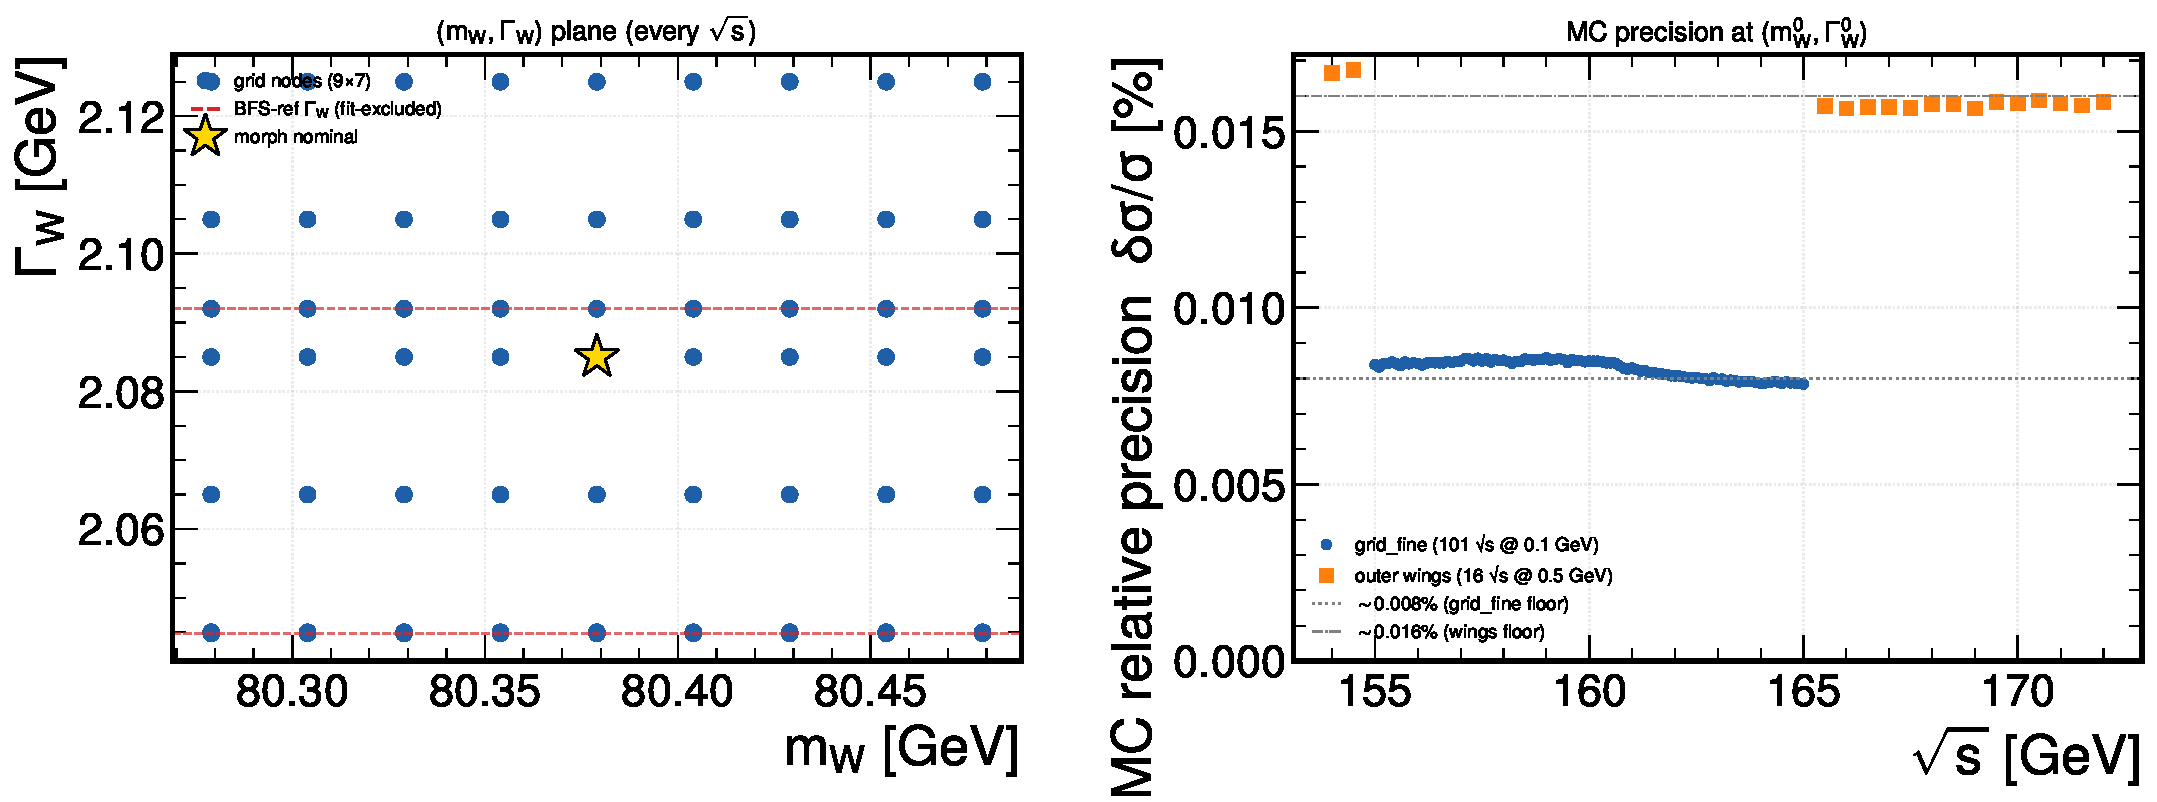
\includegraphics[width=0.95\linewidth]{morph_grid_overview}
\caption{The WHIZARD 3.1.5 grid the operational morph is built on. Left:
the $(\mW,\GammaW)$ sampling plane, a $9\times7$ rectangular grid
repeated at every $\sqrts$; the gold star marks the morph nominal
point $(\mW^0,\GammaW^0)$, the dashed red lines the two
BFS-reference $\GammaW$ values that are kept in the grid but excluded
from the morph fit (they are used later for the external closure).
Right: the per-point Monte-Carlo relative precision at
$(\mW^0,\GammaW^0)$ for the \texttt{grid\_fine} campaign (101 $\sqrts$
at 0.1-GeV spacing in $[155, 165]$~GeV) and the 0.5-GeV outer wings
taken from the highstats campaign as $\sqrts$-spline support --- flat
at $\sim$0.008\,\% inside the fine window and $\sim$0.016\,\% on the
wings. The two floors set the bands against which all morph residuals
below are compared.}
\label{fig:mv-grid}
\end{figure}

\subsection{Per-$\sqrts$ morph fits}\label{sec:morphval-axis}

At each grid $\sqrts$ the one-dimensional $\mW$ and $\GammaW$ responses are fitted with quadratics. Fig.~\ref{fig:mv-axisfits} shows the fits are adequate over the whole range: the quadratic residual is structureless and at the MC floor, a linear model is visibly insufficient, and a cubic term brings no gain.

\begin{figure}[htbp]
\centering
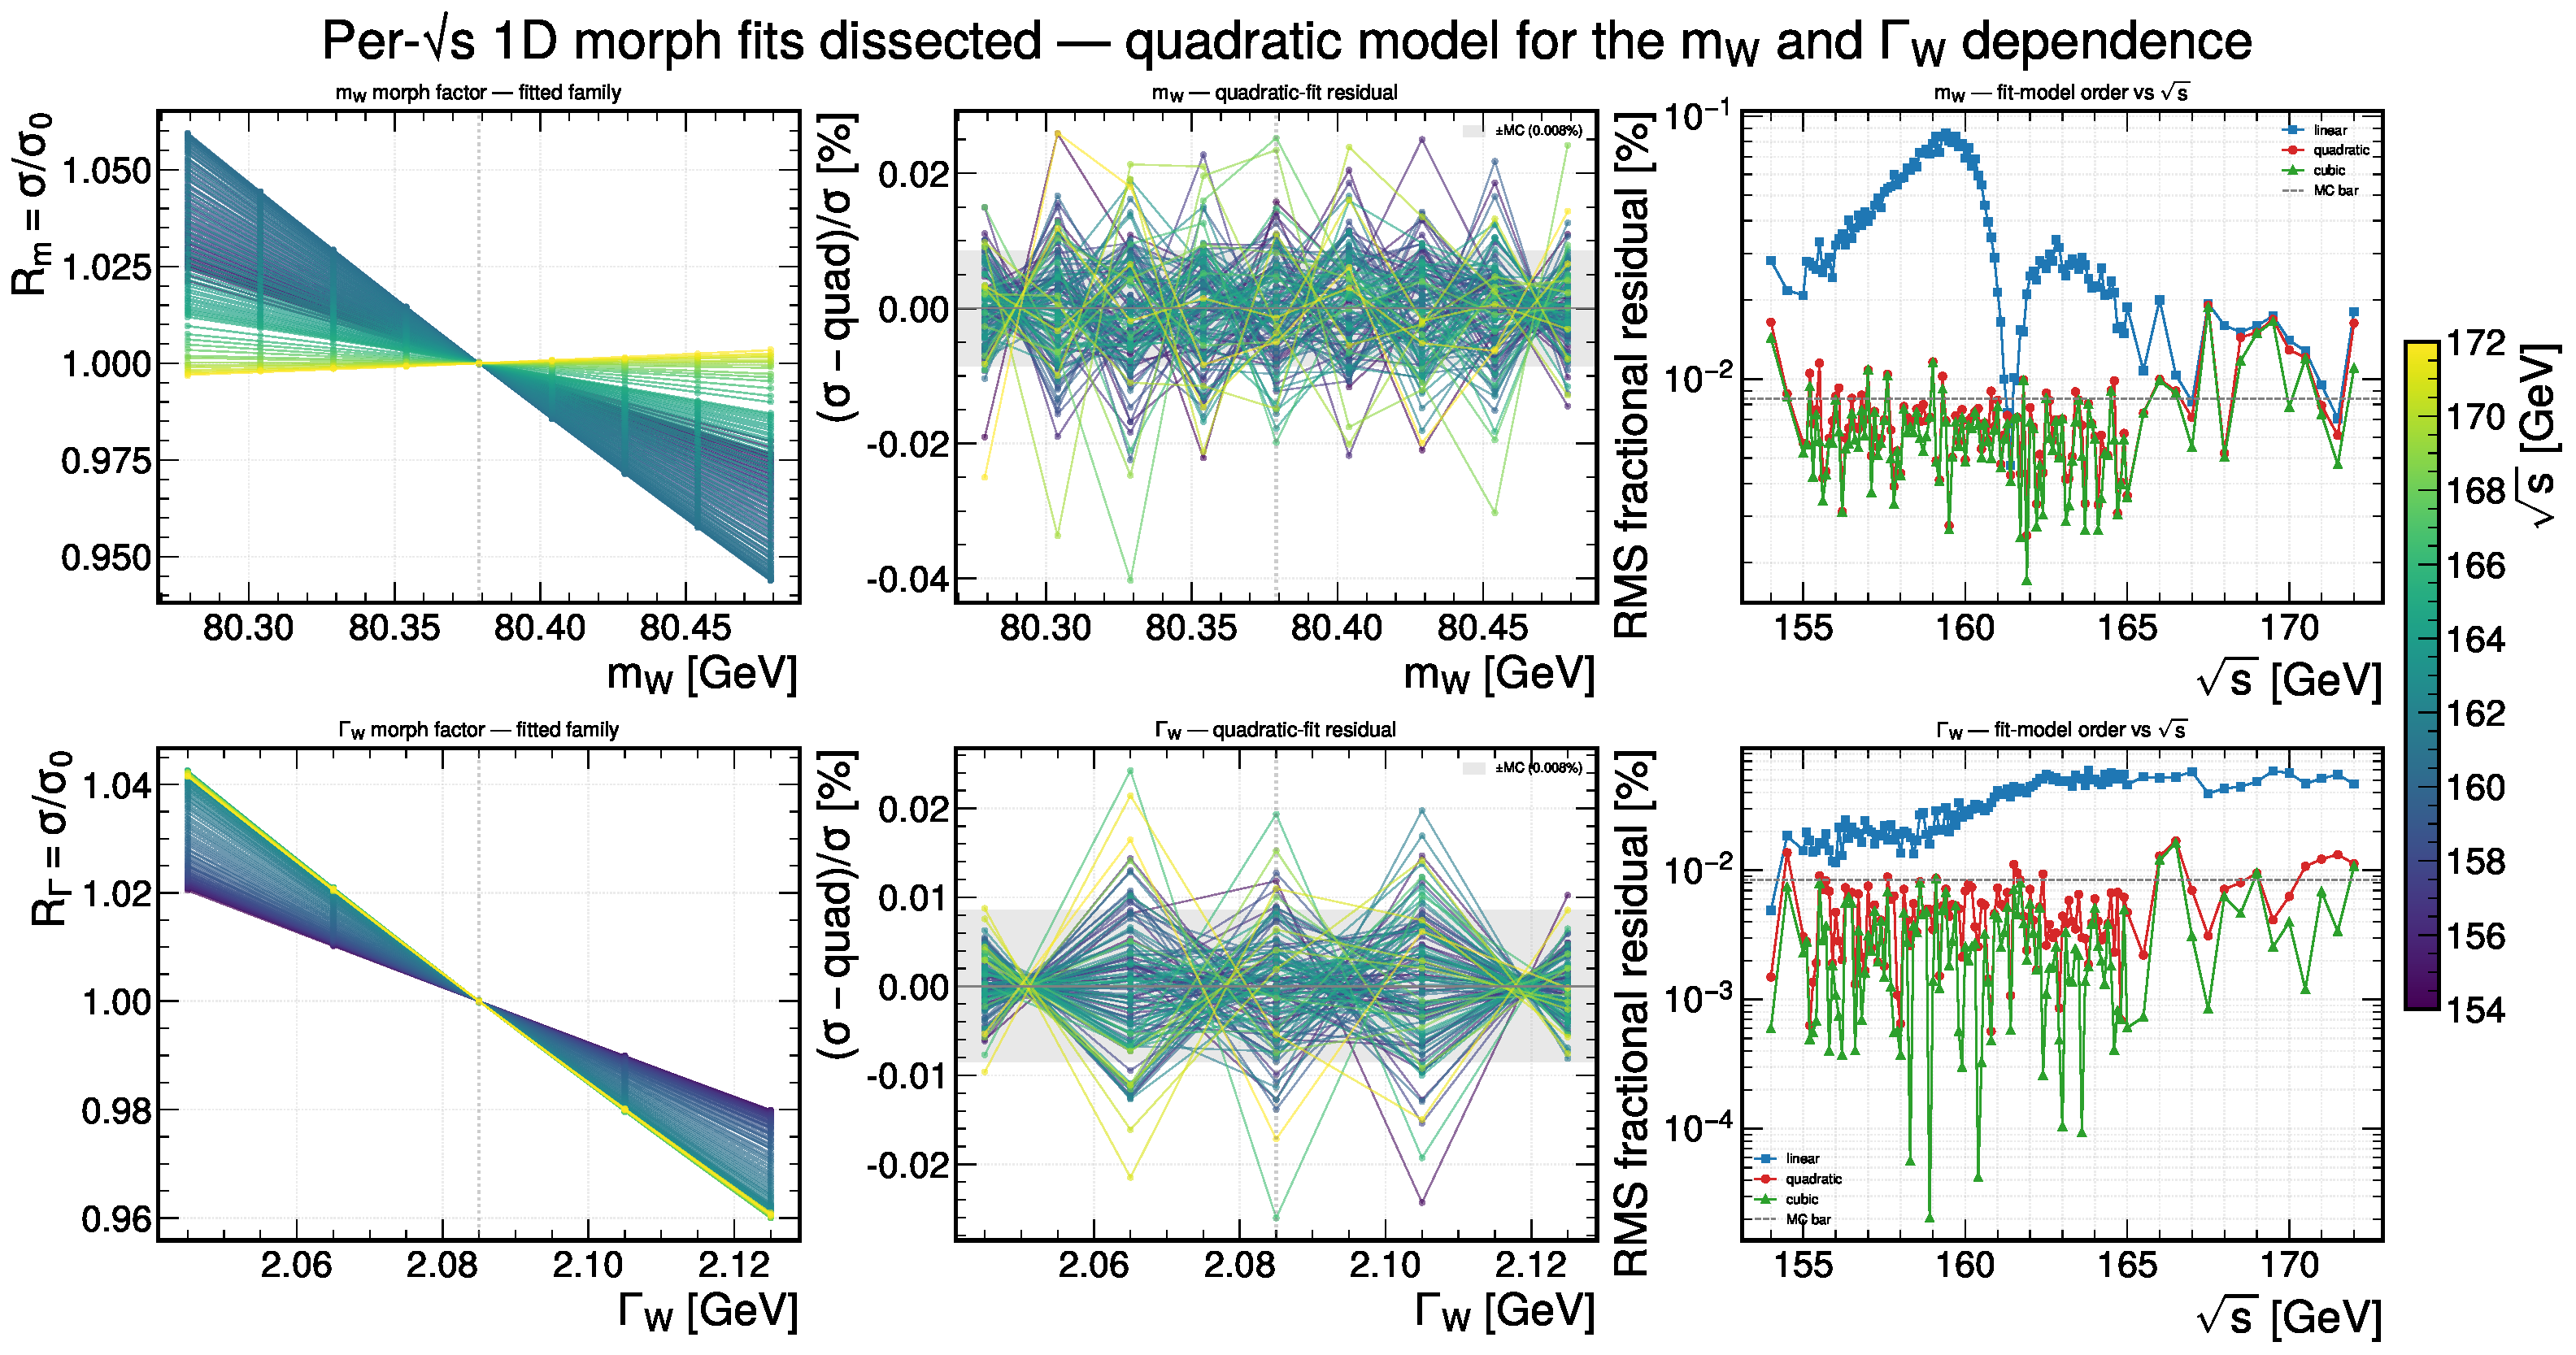
\includegraphics[width=\linewidth]{morph_axis_fits}
\caption{Dissection of the per-$\sqrts$ 1D morph fits --- top row the
$\mW$ axis, bottom row the $\GammaW$ axis, colour encoding $\sqrts$.
Left: the fitted morph factor $\mathcal{R}=\sigma/\sigma_0$ family,
showing how the curvature of each response evolves across the
threshold. Middle: the fractional residual of the quadratic fit ---
structureless and within the per-point MC band at every $\sqrts$,
i.e.\ the quadratic leaves no significant trend. Right: the RMS
fractional residual of a linear, quadratic and cubic fit as a function
of $\sqrts$; the linear fit sits several times above the MC bar, the
quadratic reaches it, and the cubic adds nothing. The quadratic is
therefore the correct model order on both axes over the whole range.}
\label{fig:mv-axisfits}
\end{figure}

\subsection{Joint coupling and the bilinear cross term}
\label{sec:morphval-cross}

The product $\sigma_0\mathcal{R}_m\mathcal{R}_\Gamma$ of the two 1D morphs misses the joint coupling near threshold. Fig.~\ref{fig:mv-cross} shows the missing piece is a clean bilinear $(\mW-\mW^0)(\GammaW-\GammaW^0)$ term, absorbed by the single scalar $\beta(\sqrts)$.

\begin{figure}[htbp]
\centering
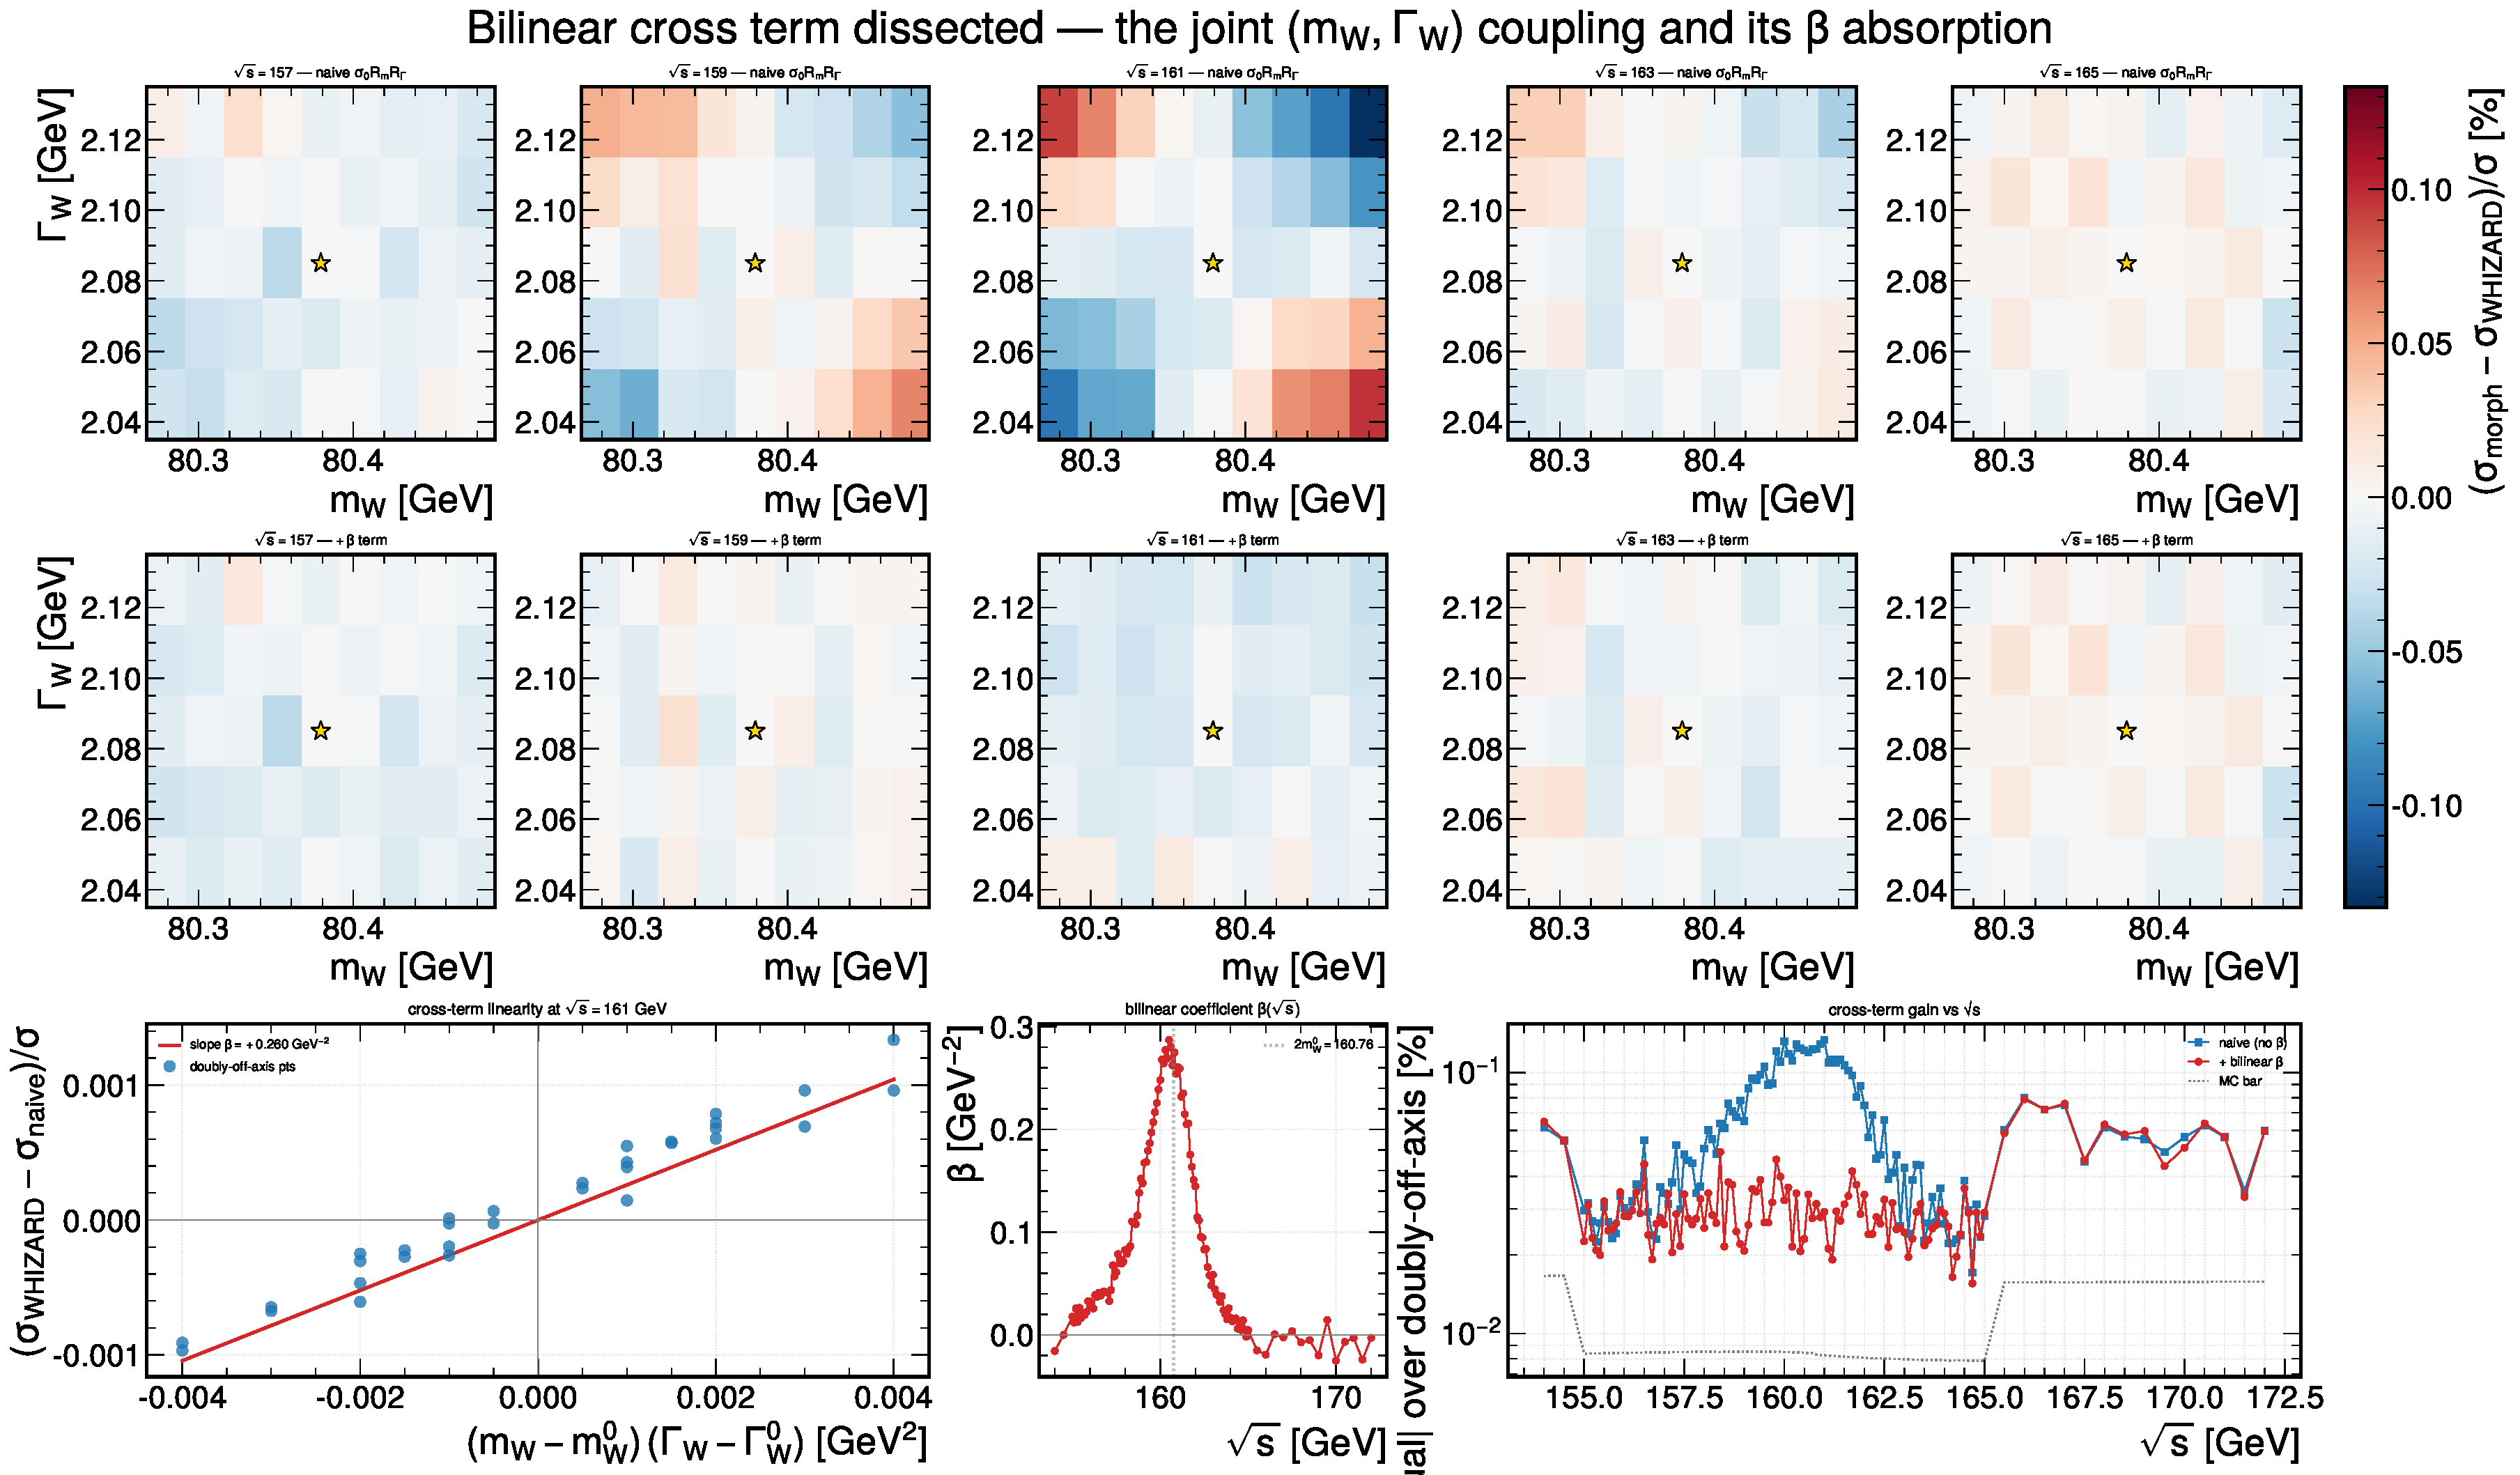
\includegraphics[width=\linewidth]{morph_cross_term}
\caption{Dissection of the bilinear cross term $\beta$. Top two rows:
the residual of the naive product morph
$\sigma_0\mathcal{R}_m\mathcal{R}_\Gamma$ and of the full morph with
the $\beta$ term, shown as $(\mW,\GammaW)$ residual maps at five
$\sqrts$ spanning the analysis range. The naive map carries a clear
$\mW\!\cdot\!\GammaW$ saddle --- opposite-sign corners --- strongest at
the threshold rise; the cross term flattens it. Bottom: (left) the
naive fractional residual is linear in
$(\mW-\mW^0)(\GammaW-\GammaW^0)$, which validates the bilinear ansatz,
with slope $\beta$; (middle) the per-$\sqrts$ fitted $\beta(\sqrts)$,
peaking near $+0.29\GeV^{-2}$ at $\sqrts\simeq160.5\GeV$ and decaying
to zero away from threshold (the $\chi^2$-smoothed curve actually
carried by the morph is shown in Fig.~\ref{fig:mv-sqrts-abs}); (right)
the maximum residual over the doubly-off-axis
points, naive versus full morph, versus $\sqrts$ --- the cross term
brings it down to the MC bar everywhere in the analysis window
(naive max 0.13\,\%, bilinear max 0.08\,\%).}
\label{fig:mv-cross}
\end{figure}

\subsection{$\sqrts$ interpolation}\label{sec:morphval-sqrts}

Between grid $\sqrts$ the eight morph quantities are carried by natural cubic splines through the denoised grid. Fig.~\ref{fig:mv-sqrts-abs} shows the quantities themselves and Fig.~\ref{fig:mv-sqrts} the deviation of the raw per-$\sqrts$ fit from the denoised curve actually used; Fig.~\ref{fig:mv-sqrtsval} is a blind test in which the morph is rebuilt from a 0.2-GeV thinned subset of \texttt{grid\_fine} and used to predict the held-out 0.1-GeV midpoints, and Fig.~\ref{fig:mv-4dloo} the standard leave-one-out cross-check on the full grid.

\begin{figure}[htbp]
\centering
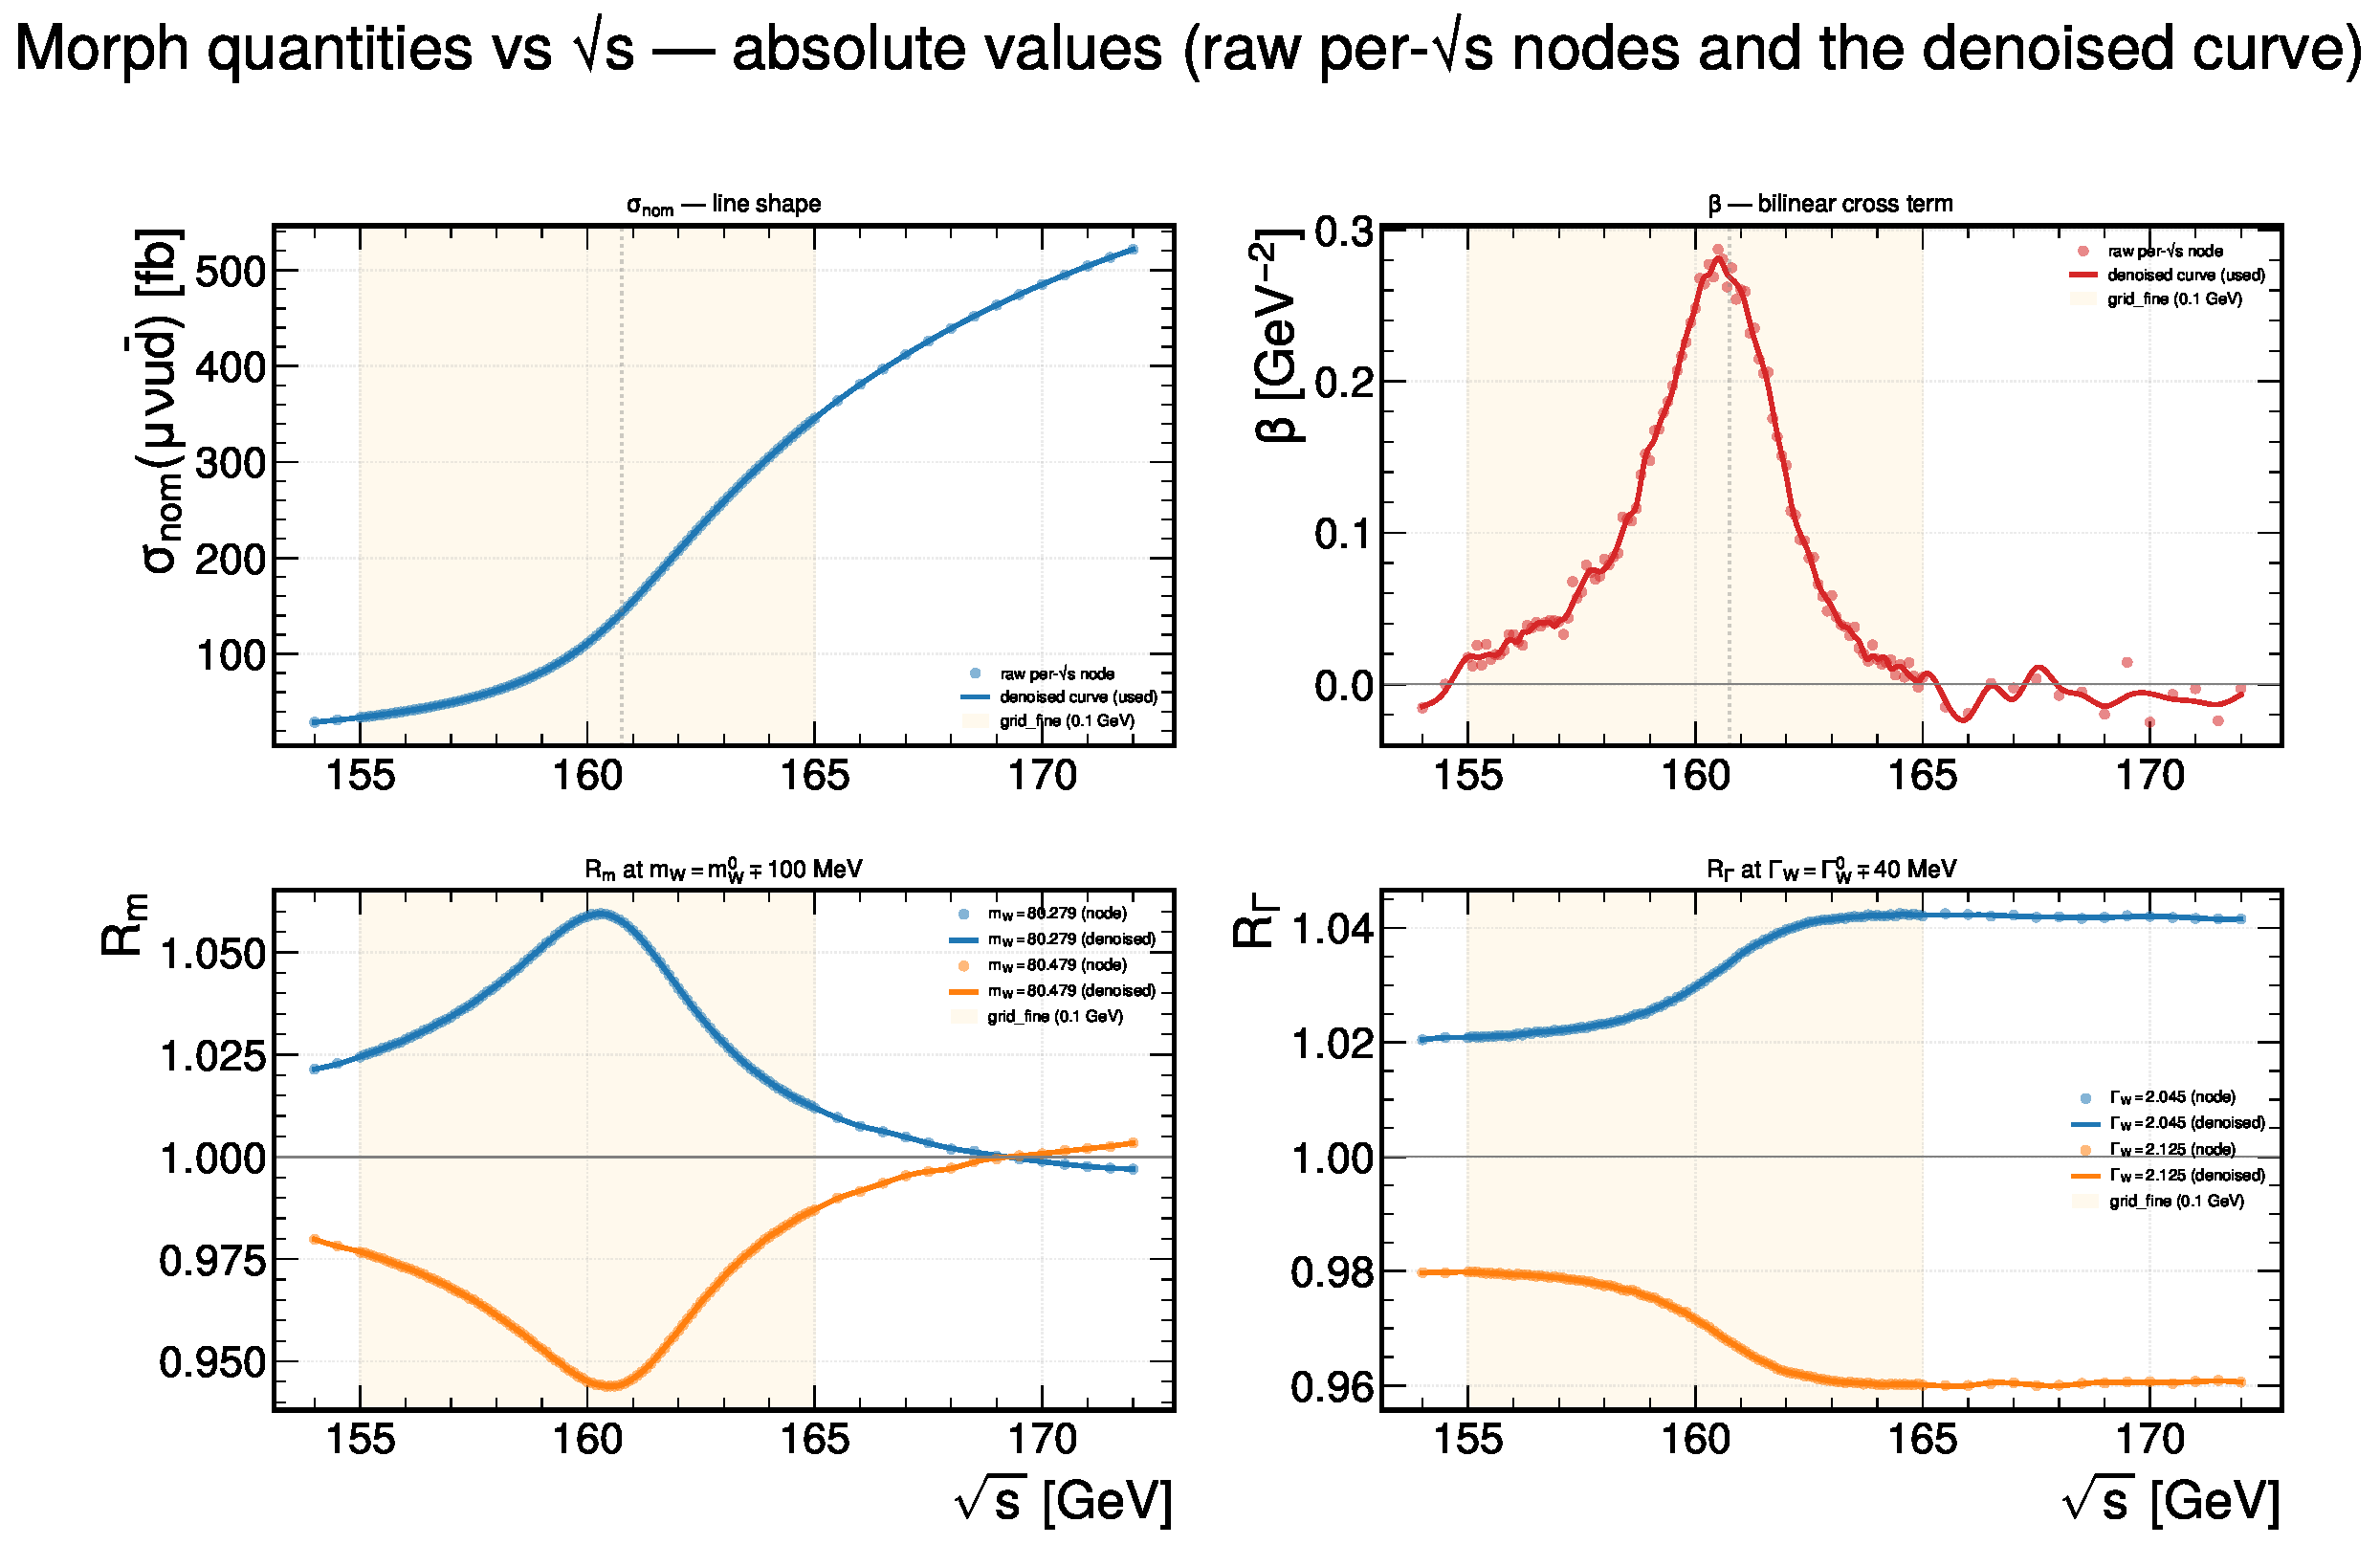
\includegraphics[width=0.92\linewidth]{morph_sqrts_quantities}
\caption{The morph quantities as a function of $\sqrts$ --- absolute
values. Points are the raw per-$\sqrts$ fit nodes, the line the
denoised curve the operational morph carries. The orange band marks
the \texttt{grid\_fine} window (0.1-GeV $\sqrts$ step); outside it the
0.5-GeV wings are used as spline support. $\sigma_0$ is the steep
threshold line shape; $\beta$ is the bilinear cross term, with the
per-$\sqrts$ fit peaking near $+0.29\GeV^{-2}$ at the rise and the
$\chi^2$-smoothed curve carried by the morph at $+0.27\GeV^{-2}$;
$R_m$ and $R_\Gamma$ are the $m_W$ / $\GammaW$ morph factors, shown
at $\mp100\MeV$ and $\mp40\MeV$ off nominal. Fig.~\ref{fig:mv-sqrts}
shows the same quantities as the deviation from the denoised curve.}
\label{fig:mv-sqrts-abs}
\end{figure}

\begin{figure}[htbp]
\centering
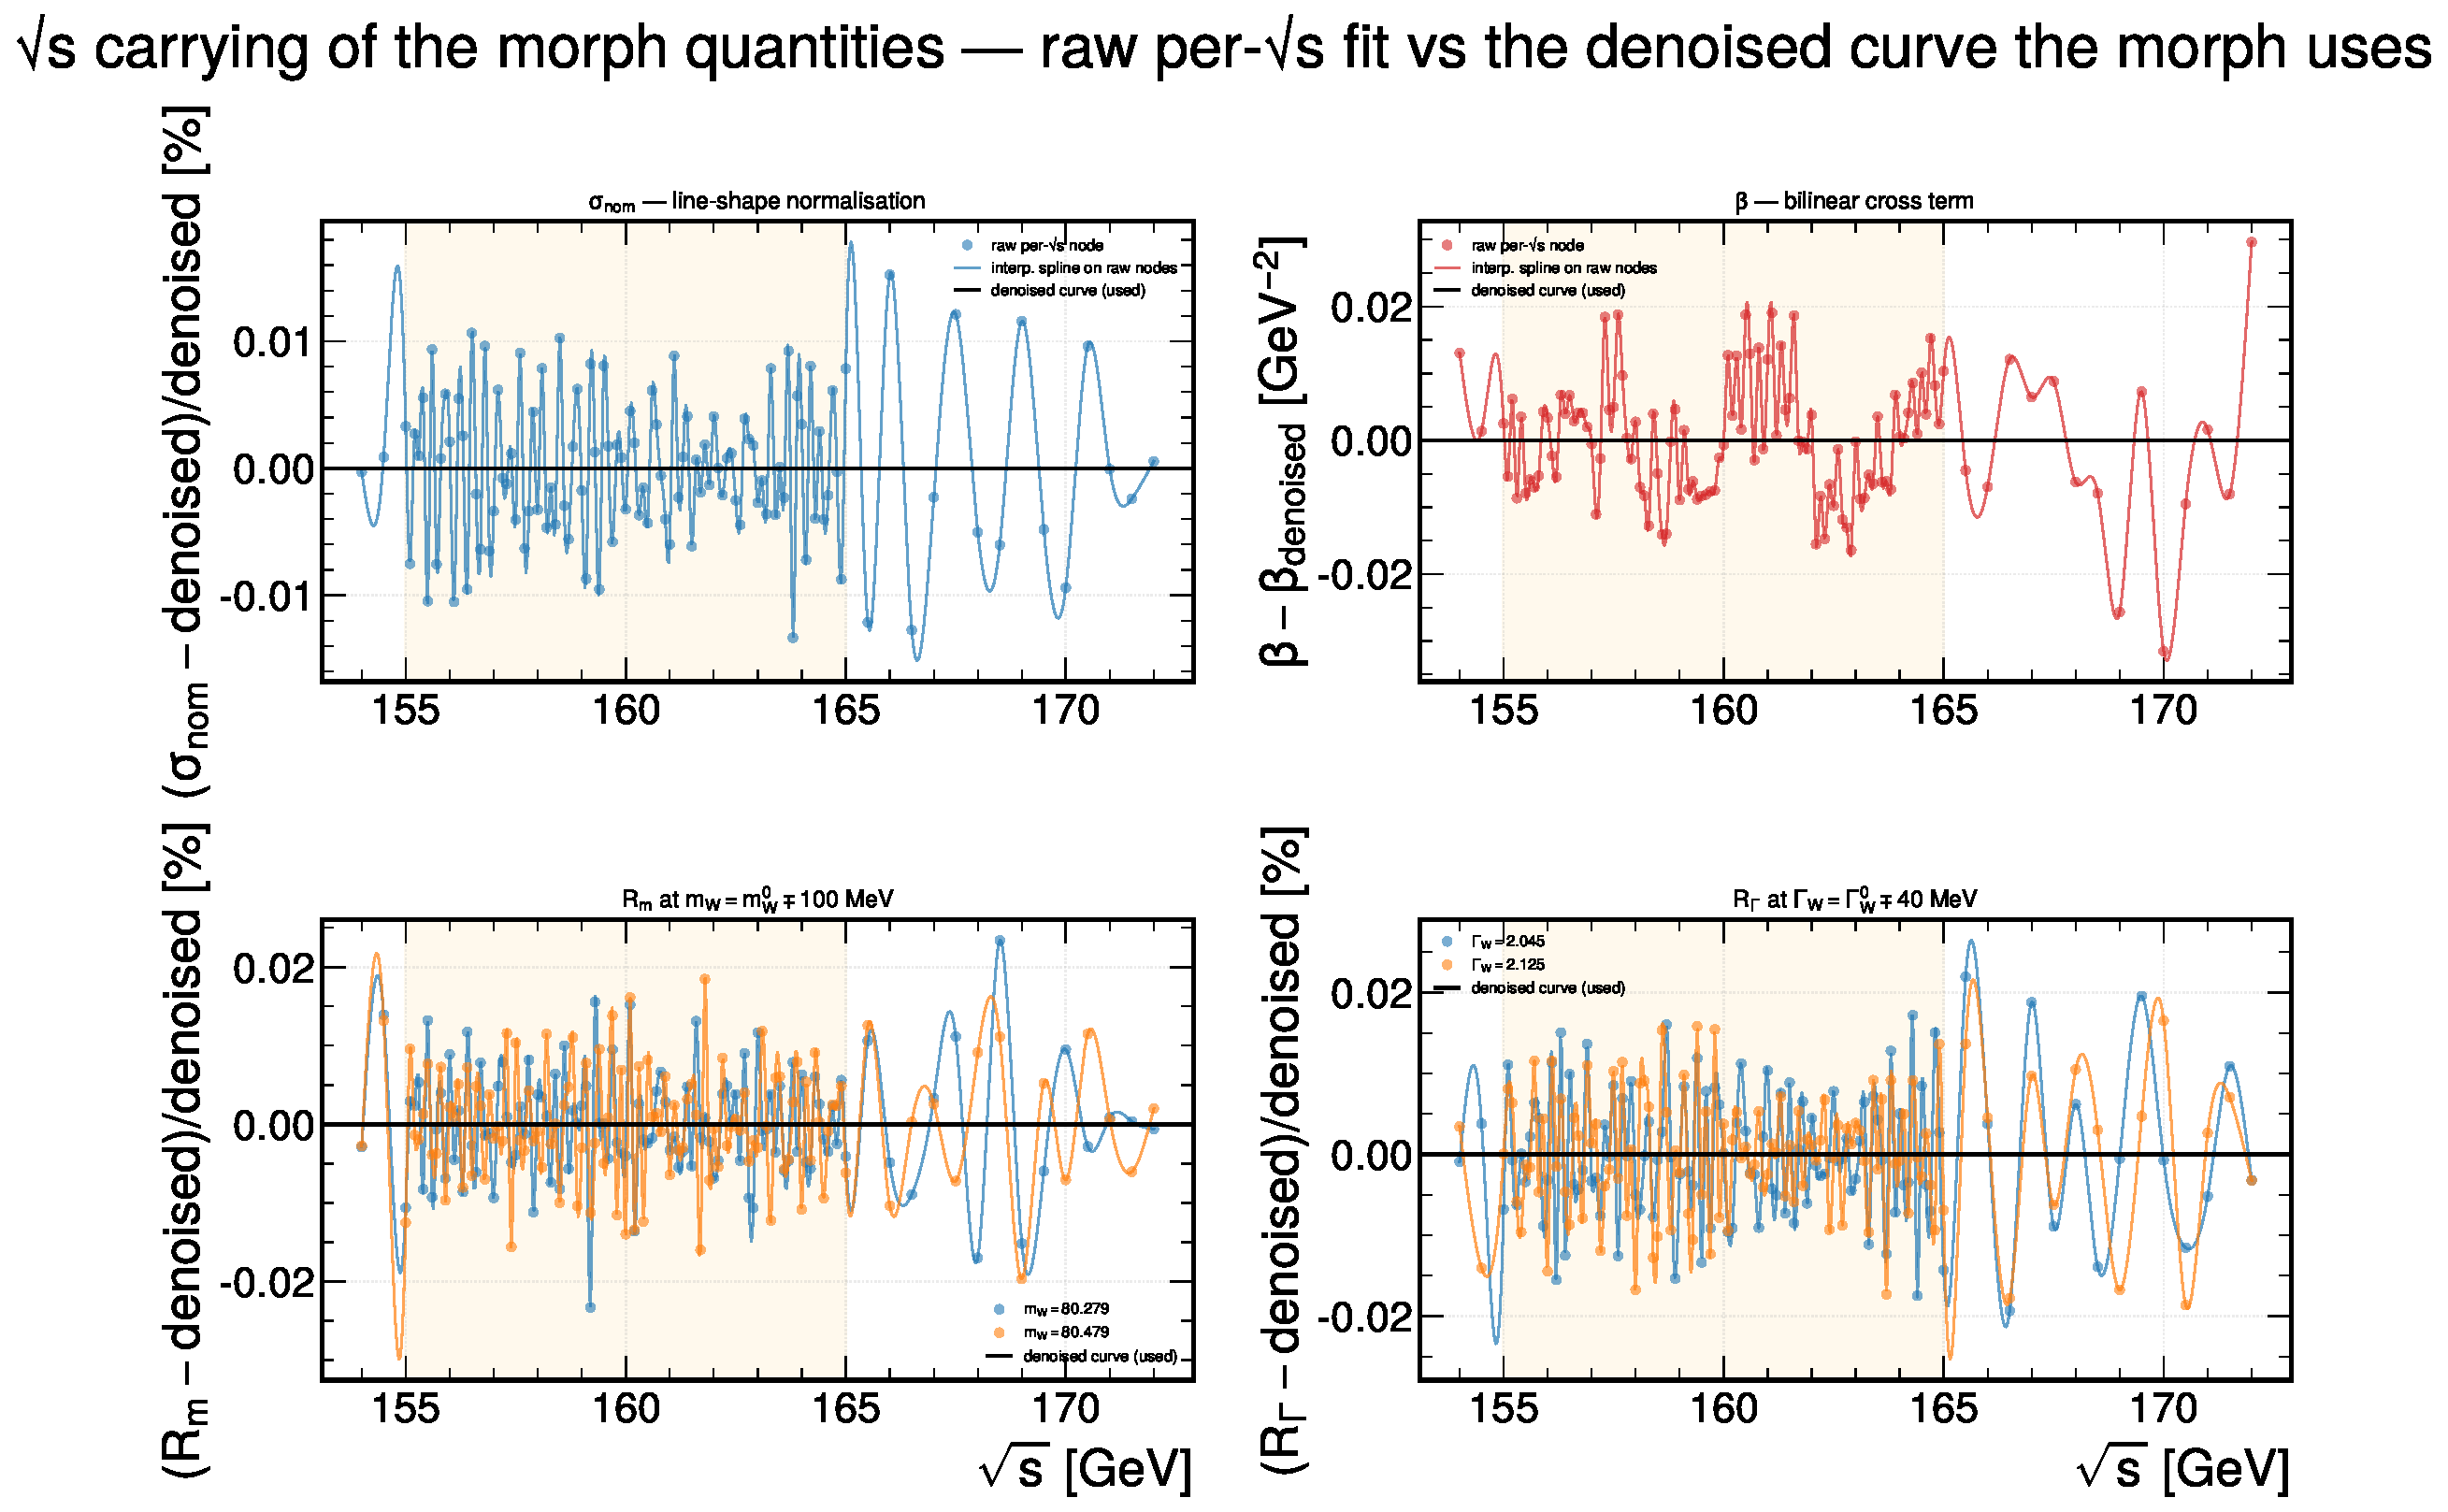
\includegraphics[width=0.92\linewidth]{morph_sqrts_interpolation}
\caption{The $\sqrts$ carrying of the morph quantities, each shown as
the deviation from the denoised curve the operational morph uses (the
zero line). Points are the raw per-$\sqrts$ fit nodes; the thin line is
an interpolating cubic spline through them --- the ripple that would be
propagated if the grid were not denoised. With \texttt{grid\_fine} at
$\sim$0.008\,\% MC the per-node fluctuation is already small and the
denoising acts as a thin smoothing pass on top of an already-clean
spline; on the noisier 0.5-GeV wings (orange band excluded) it still
visibly tightens the curve. \code{denoise_grid} removes the ripple by
$\chi^2$-smoothing the slowly-varying ratios $\sigma/\sigma_0$ along
$\sqrts$ and averaging $\sigma_0$ across the $(\mW,\GammaW)$ plane,
so the morph carries the smooth zero-line curve. $\beta$ receives an
additional $\chi^2$-targeted smoothing along $\sqrts$ (with weights
$1/\sigma_\beta$ from the per-$\sqrts$ bilinear LSQ); the zero line
here is therefore the smoothed $\beta$, and the raw nodes scatter
around it.}
\label{fig:mv-sqrts}
\end{figure}

\begin{figure}[htbp]
\centering
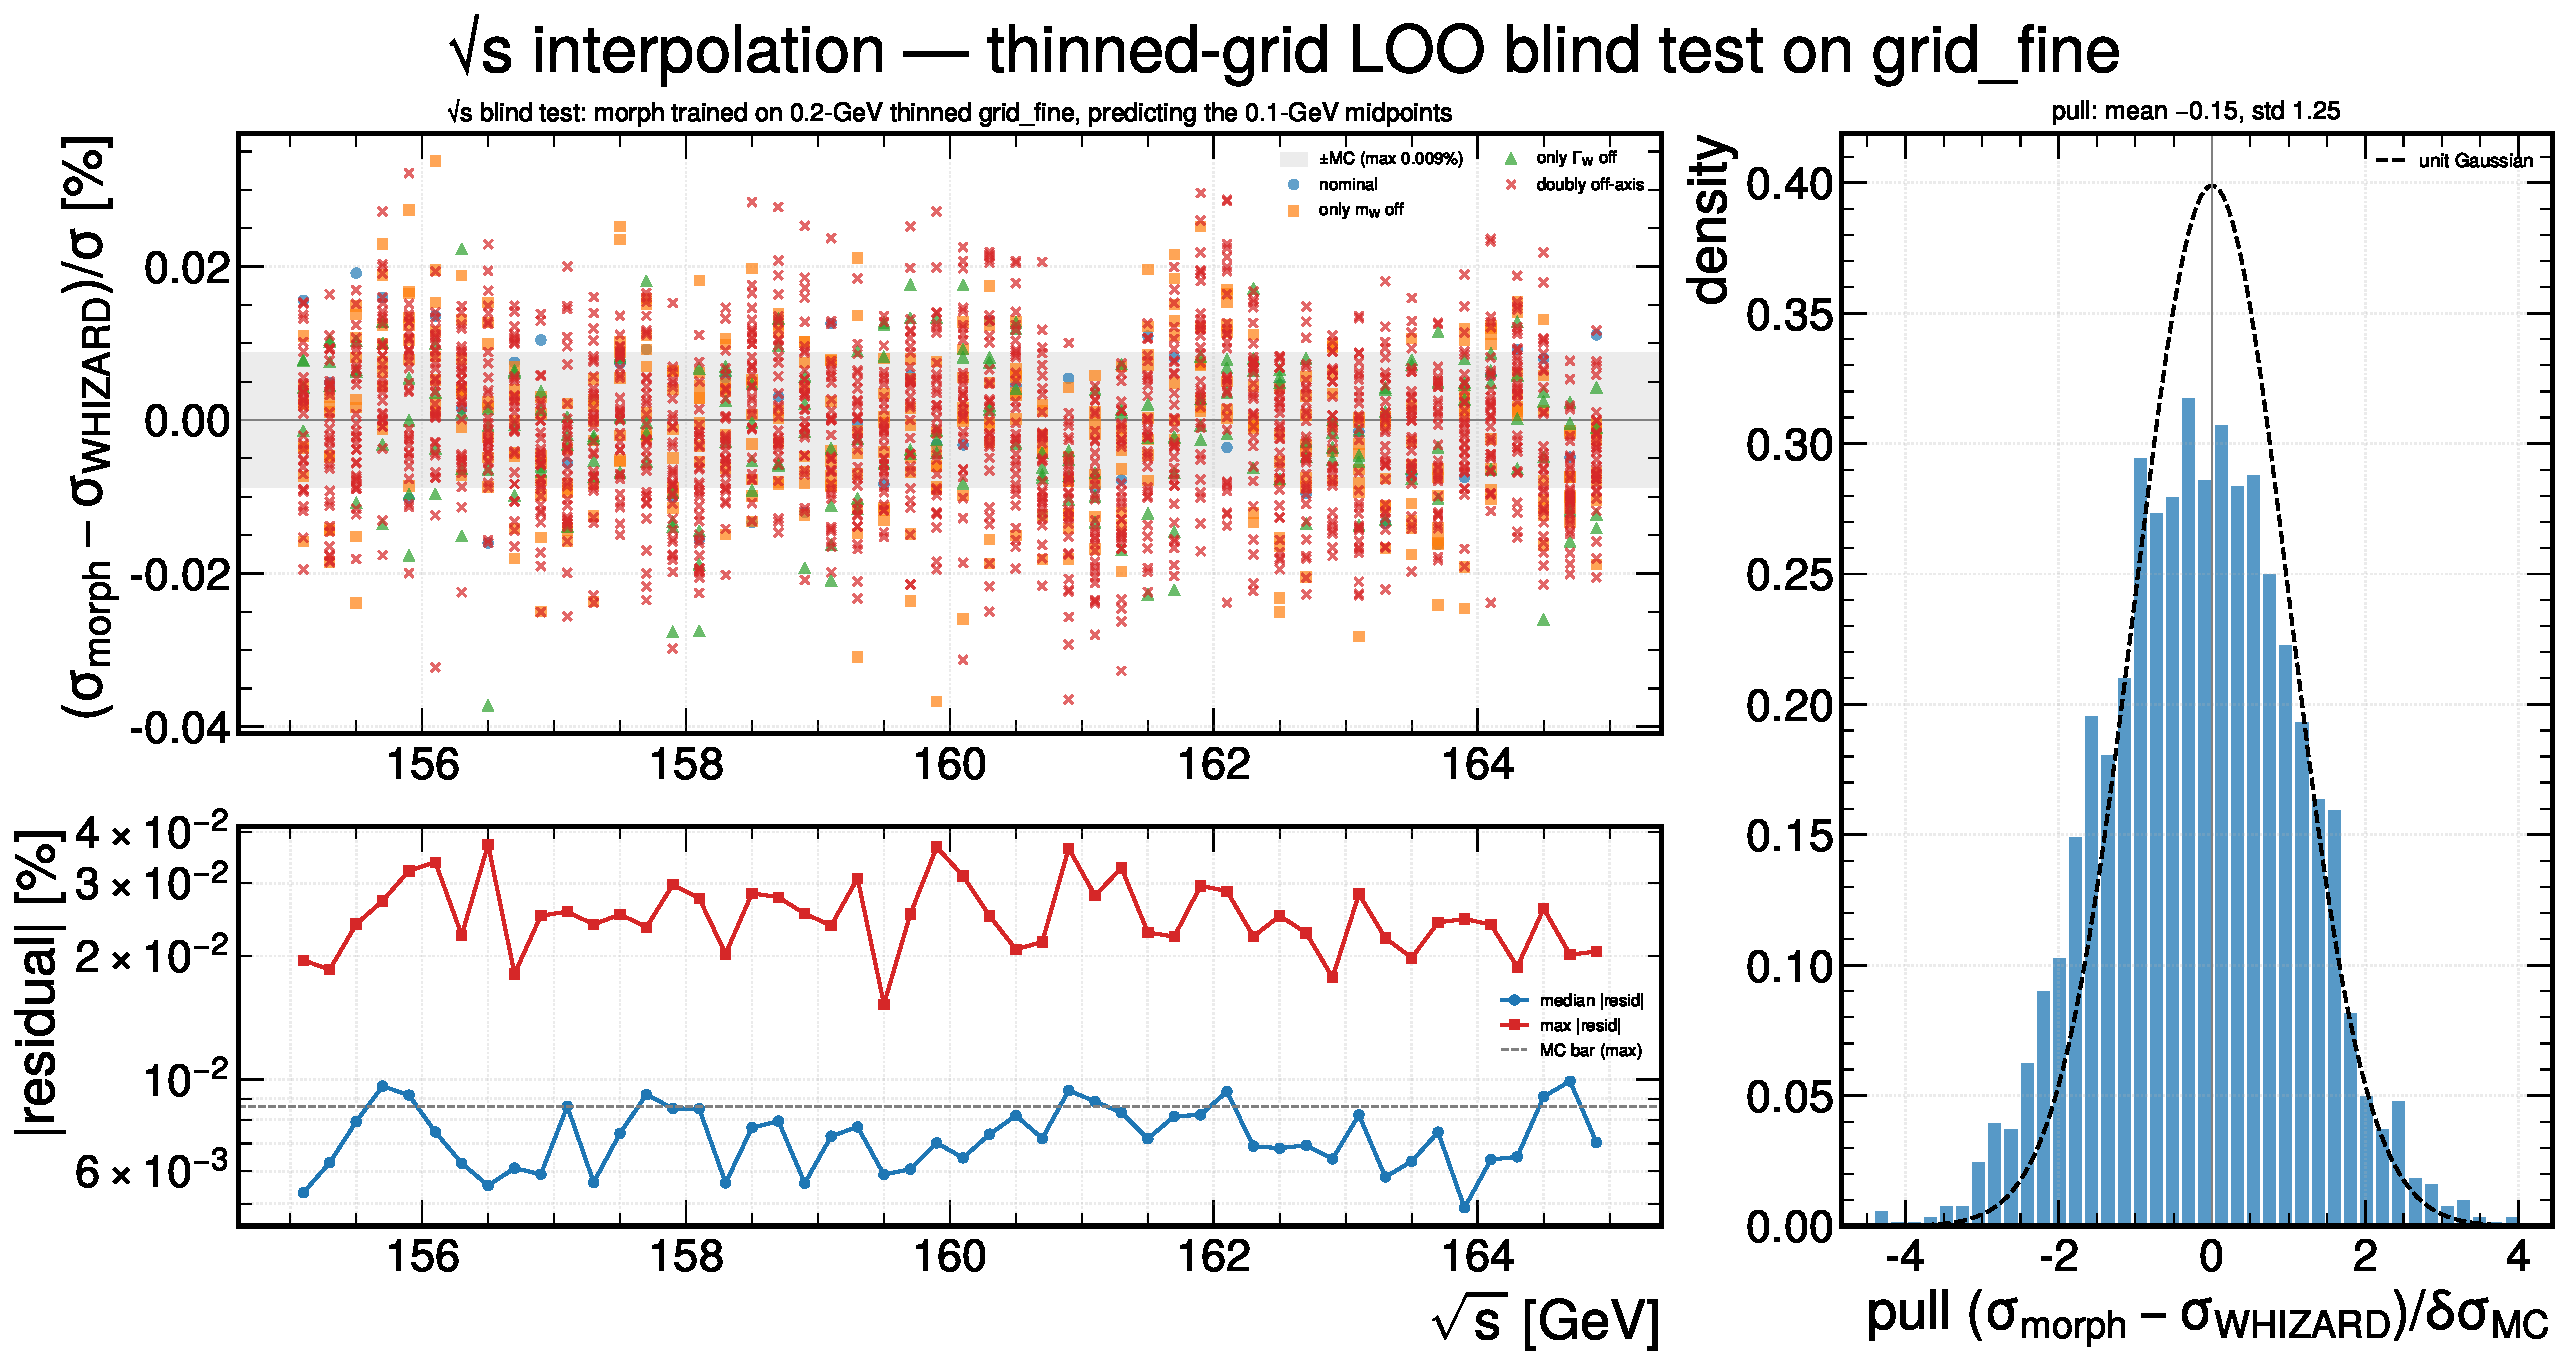
\includegraphics[width=0.95\linewidth]{morph_sqrts_validation}
\caption{Blind test of the $\sqrts$ interpolation, by thinned-grid
leave-one-out on \texttt{grid\_fine}. The morph is rebuilt from the
0.2-GeV subset (\textit{i.e.}\ keeping every other $\sqrts$ node) plus
the 0.5-GeV wings, and used to predict the 50 held-out 0.1-GeV
midpoints --- 2250 points the training spline never sees, at the full
\texttt{grid\_fine} step distance from their nearest training nodes.
This is stronger than leave-one-out, which removes a node the spline
would otherwise anchor on. Left: the per-point residual vs $\sqrts$
(top) and its median and maximum (bottom) --- MC-bar limited, maximum
$0.037\,\%$ and median $0.007\,\%$. Right: the pull
$(\sigma_\text{morph}-\sigma_\text{WHIZARD})/
\delta\sigma_\text{MC}$, centred on zero (no systematic bias); its
width $\sim$1.25, demonstrating the morph prediction is
interpolation-limited rather than dominated by propagated node noise.}
\label{fig:mv-sqrtsval}
\end{figure}

\begin{figure}[htbp]
\centering
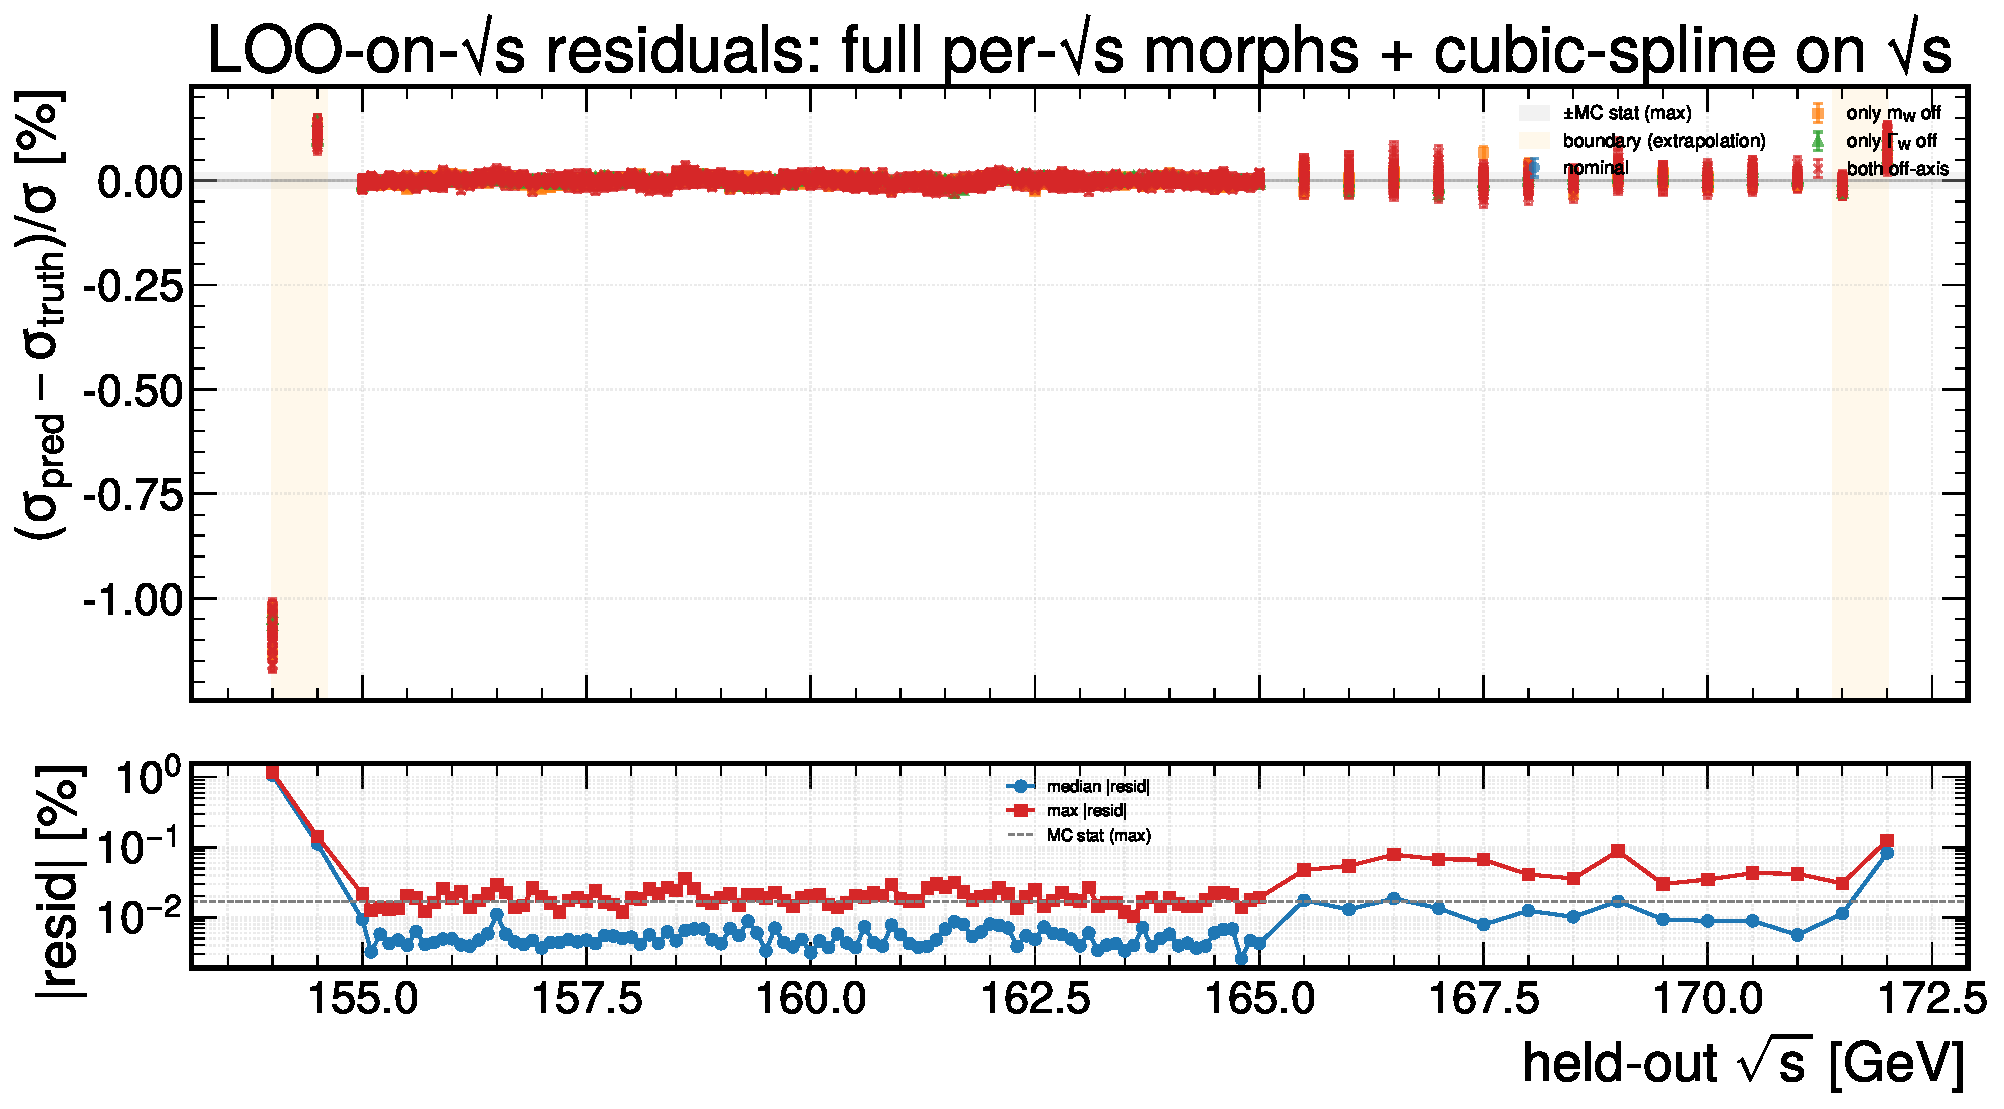
\includegraphics[width=0.95\linewidth]{morph_4d_morphing_loo}
\caption{Leave-one-out cross-validation on the $\sqrts$ axis: each grid
$\sqrts_i$ is held out, the cubic splines of the eight morph
quantities are refitted from the remaining nodes, and the full
$(\mW,\GammaW)$ plane is predicted at $\sqrts_i$. Top: per-point
residuals coloured by axis class. Bottom (log scale): median and
maximum $|\text{residual}|$ vs $\sqrts$. The interior is MC-bar
limited (median $0.005\,\%$, max $0.088\,\%$); the spikes at the two
extreme $\sqrts$ are LOO extrapolation artifacts --- the operational
interpolator never leaves the grid. The thinned-grid blind test of
Fig.~\ref{fig:mv-sqrtsval} is the leak-free companion measure.}
\label{fig:mv-4dloo}
\end{figure}

\subsection{Held-out and external closure}\label{sec:morphval-closure}

Three independent closure tests bound the total morph error: held-out
WHIZARD points at 1-MeV $(\mW,\GammaW)$ spacing
(Fig.~\ref{fig:mv-substep}); a dedicated sub-MeV $(\mW,\GammaW)$
held-out campaign at $\sim$0.005\,\% MC
(Fig.~\ref{fig:mv-validate-fine}); and the published BFS WHIZARD 4f
Born tables (Fig.~\ref{fig:mv-bfs}).

\begin{figure}[htbp]
\centering
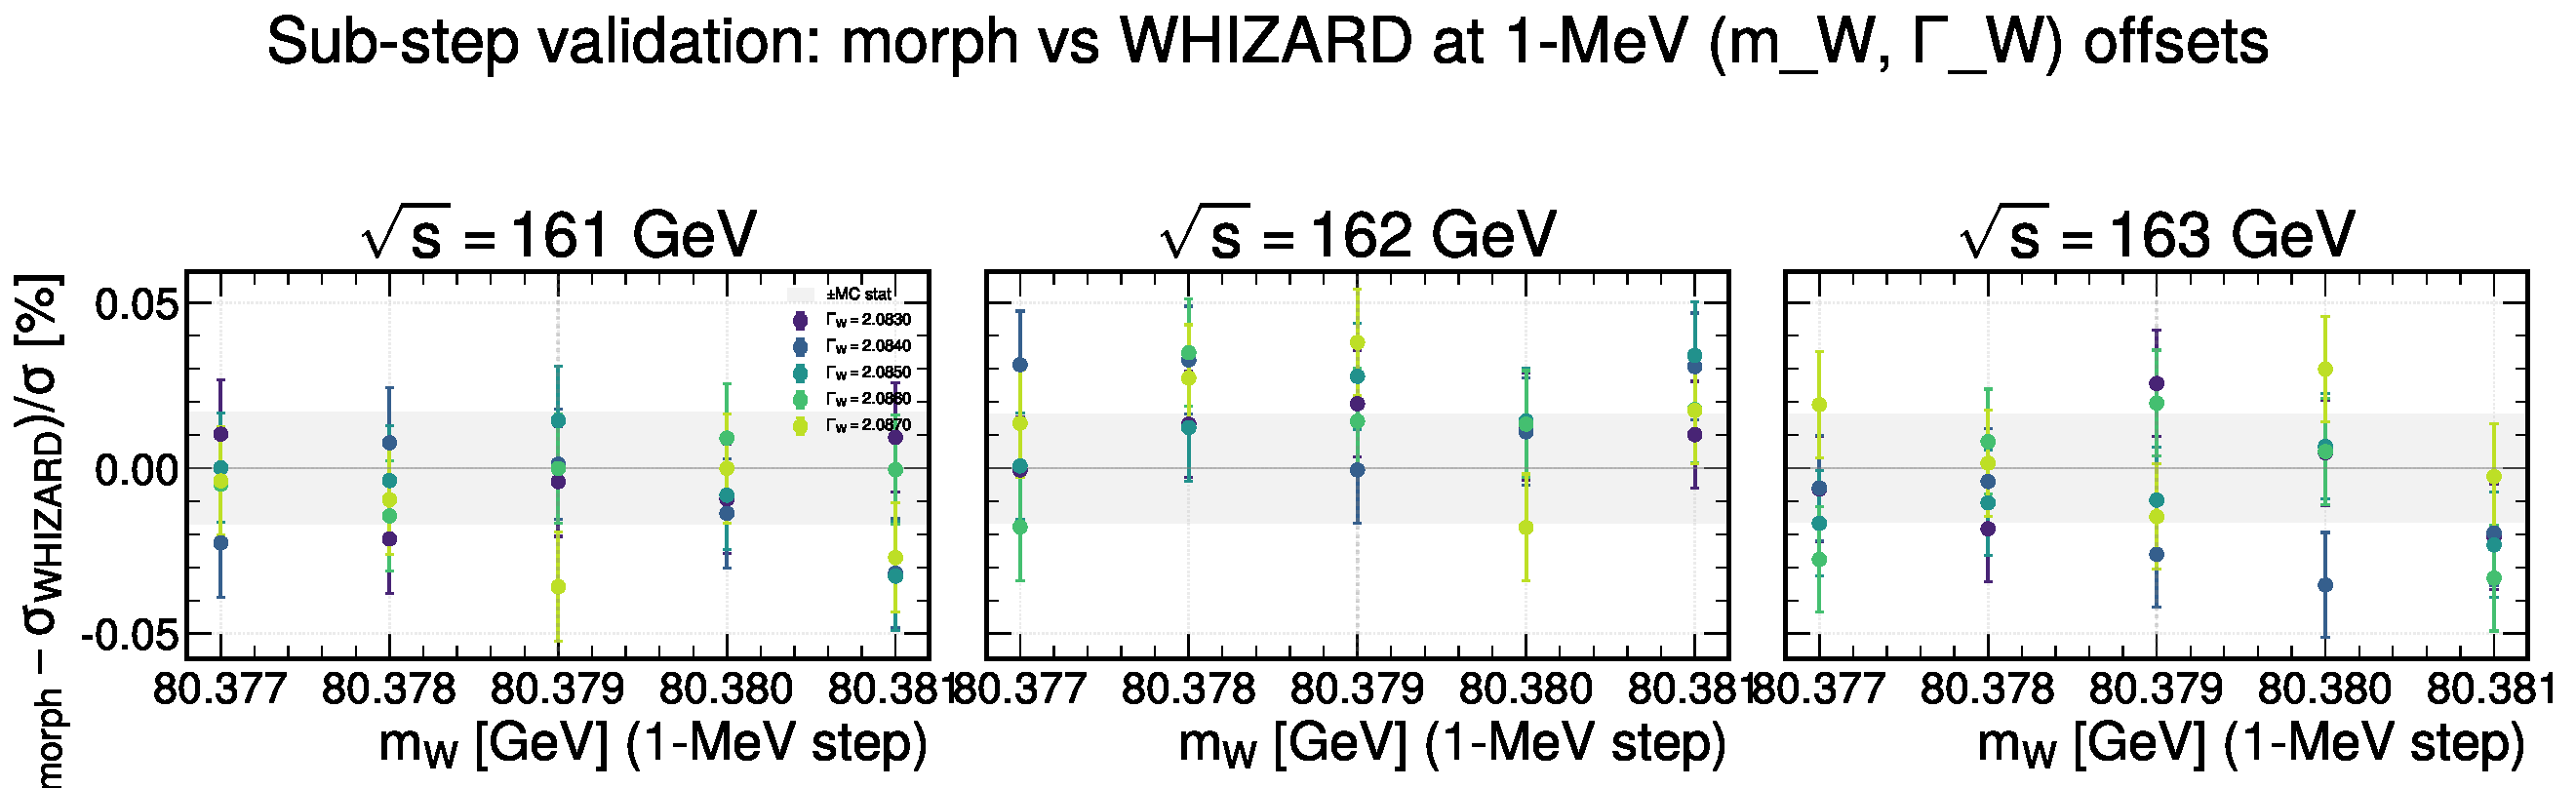
\includegraphics[width=\linewidth]{morph_validate_substep}
\caption{Held-out closure at sub-grid resolution. A dedicated WHIZARD
campaign generated a $5\times5$ $(\mW,\GammaW)$ plane at 1-MeV steps
for $\sqrts\in\{161,162,163\}\GeV$; none of these points enters the
morph. The residual $(\sigma_\text{morph}-\sigma_\text{WHIZARD})/\sigma$
scatters within the MC band with no trend --- maximum $0.038\,\%$,
median $0.009$--$0.018\,\%$ --- so the morph is MeV-safe at the
$(\mW,\GammaW)$ resolution of the fit.}
\label{fig:mv-substep}
\end{figure}

\begin{figure}[htbp]
\centering
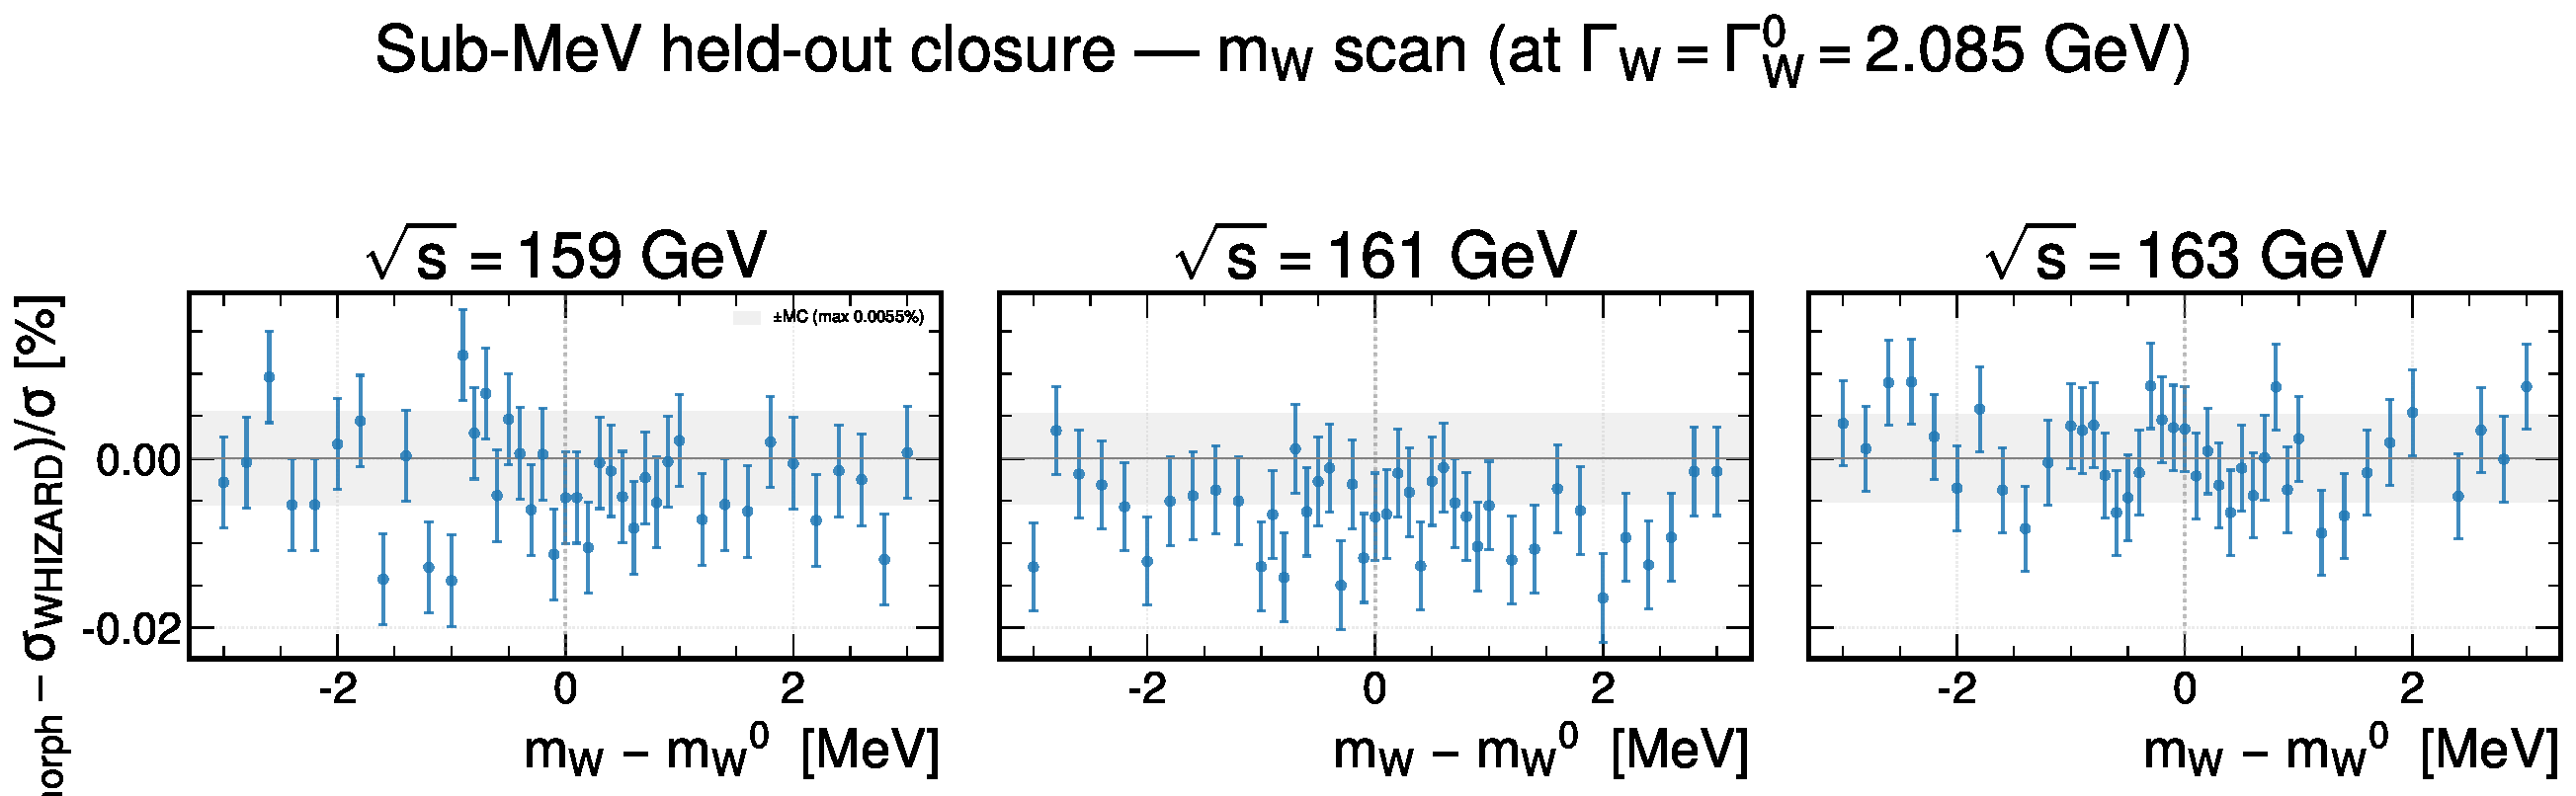
\includegraphics[width=\linewidth]{morph_validate_fine_mW}\\[2pt]
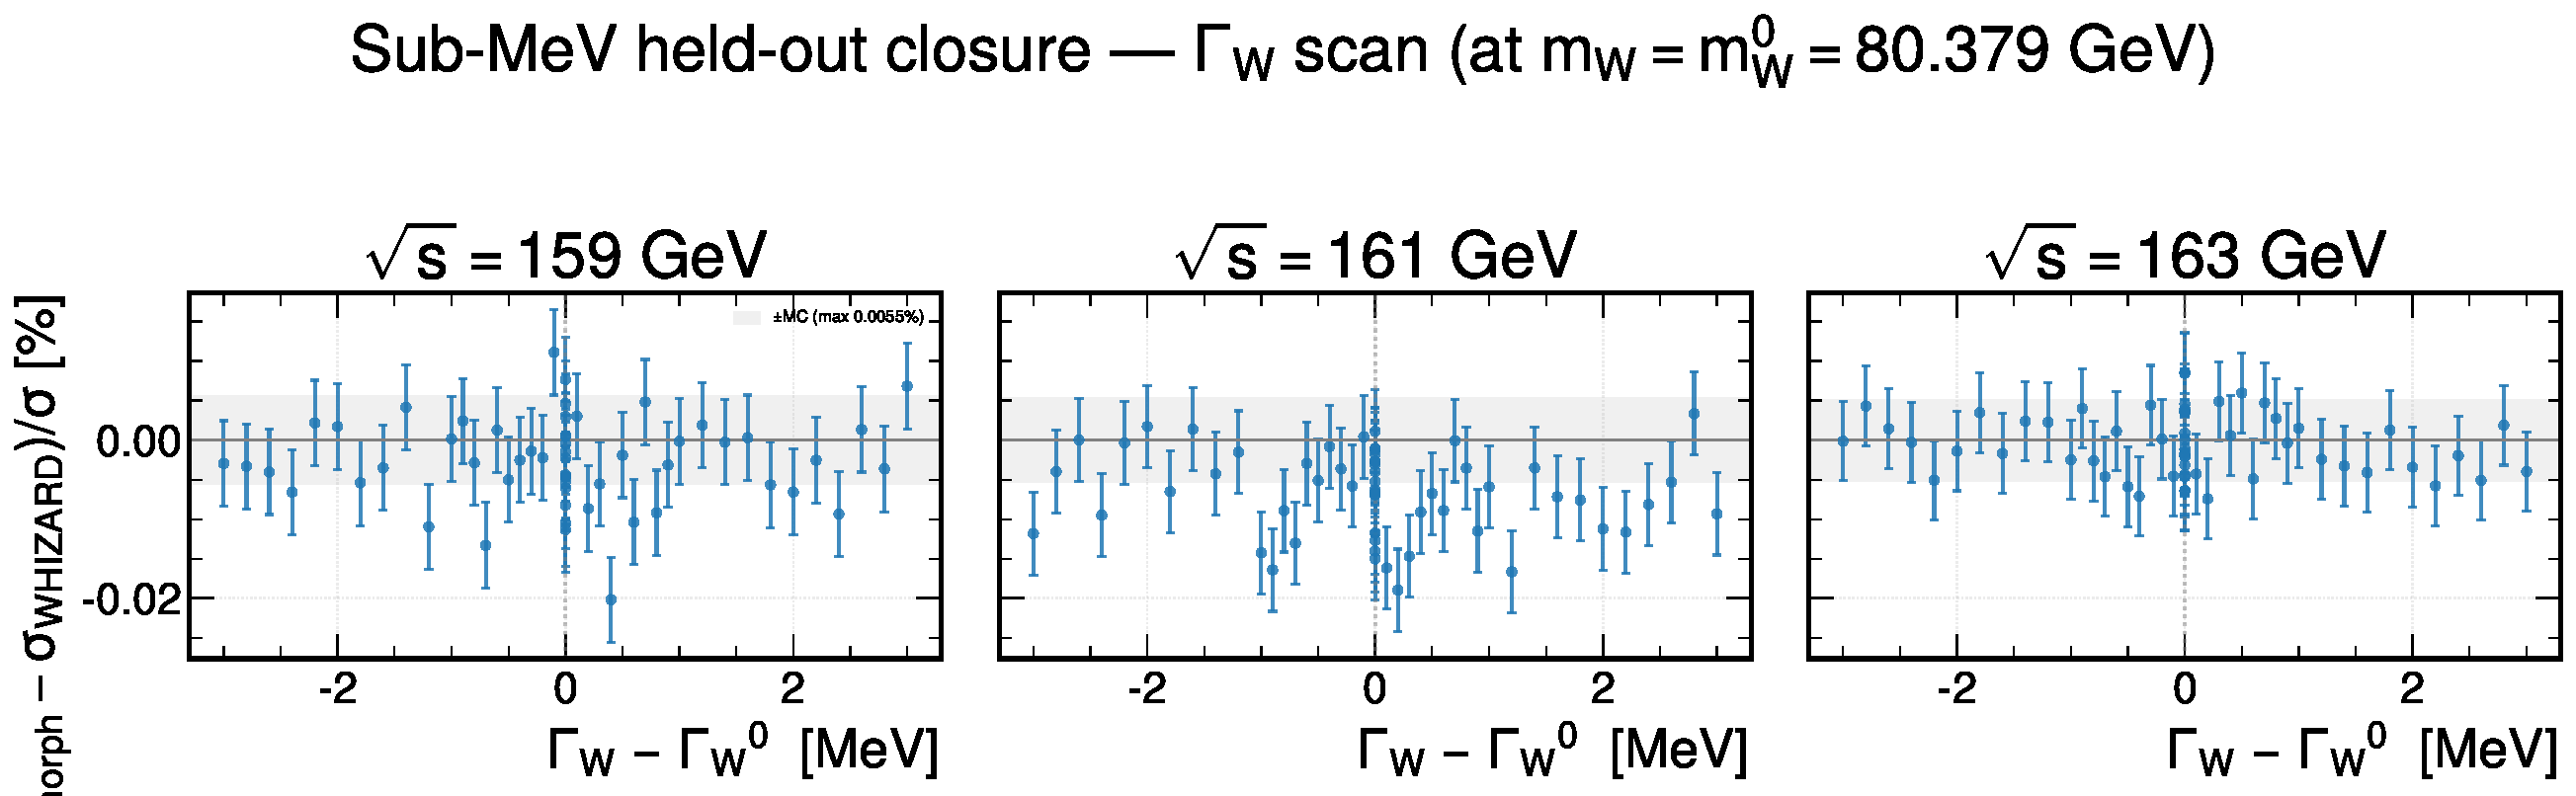
\includegraphics[width=\linewidth]{morph_validate_fine_gW}
\caption{Sub-MeV held-out closure against the dedicated
\texttt{grid\_validate\_fine} campaign --- 1D scans of $m_W$ (top,
at $\GammaW=\GammaW^0=2.085\GeV$) and $\GammaW$ (bottom, at
$m_W=m_W^0=80.379\GeV$) at 0.1-MeV steps to $\pm 1\MeV$ and 0.2-MeV to
$\pm 3\MeV$, on three $\sqrts$ slices $\in\{159,161,163\}\GeV$, at
$\sim$0.005\,\% MC. None of these points enters the morph fit. The
residuals scatter inside the MC band on both axes with no systematic
trend; the overall maximum is $0.020\,\%$ and the median $0.004\,\%$,
so the morph is sub-MeV-safe at the $(\mW,\GammaW)$ working resolution
of the fit. The 0.005\,\% MC bar cleanly resolves the 0.019\,\%
$\sigma$ shift of a 0.1-MeV $m_W$ step on this curve.}
\label{fig:mv-validate-fine}
\end{figure}

\begin{figure}[htbp]
\centering
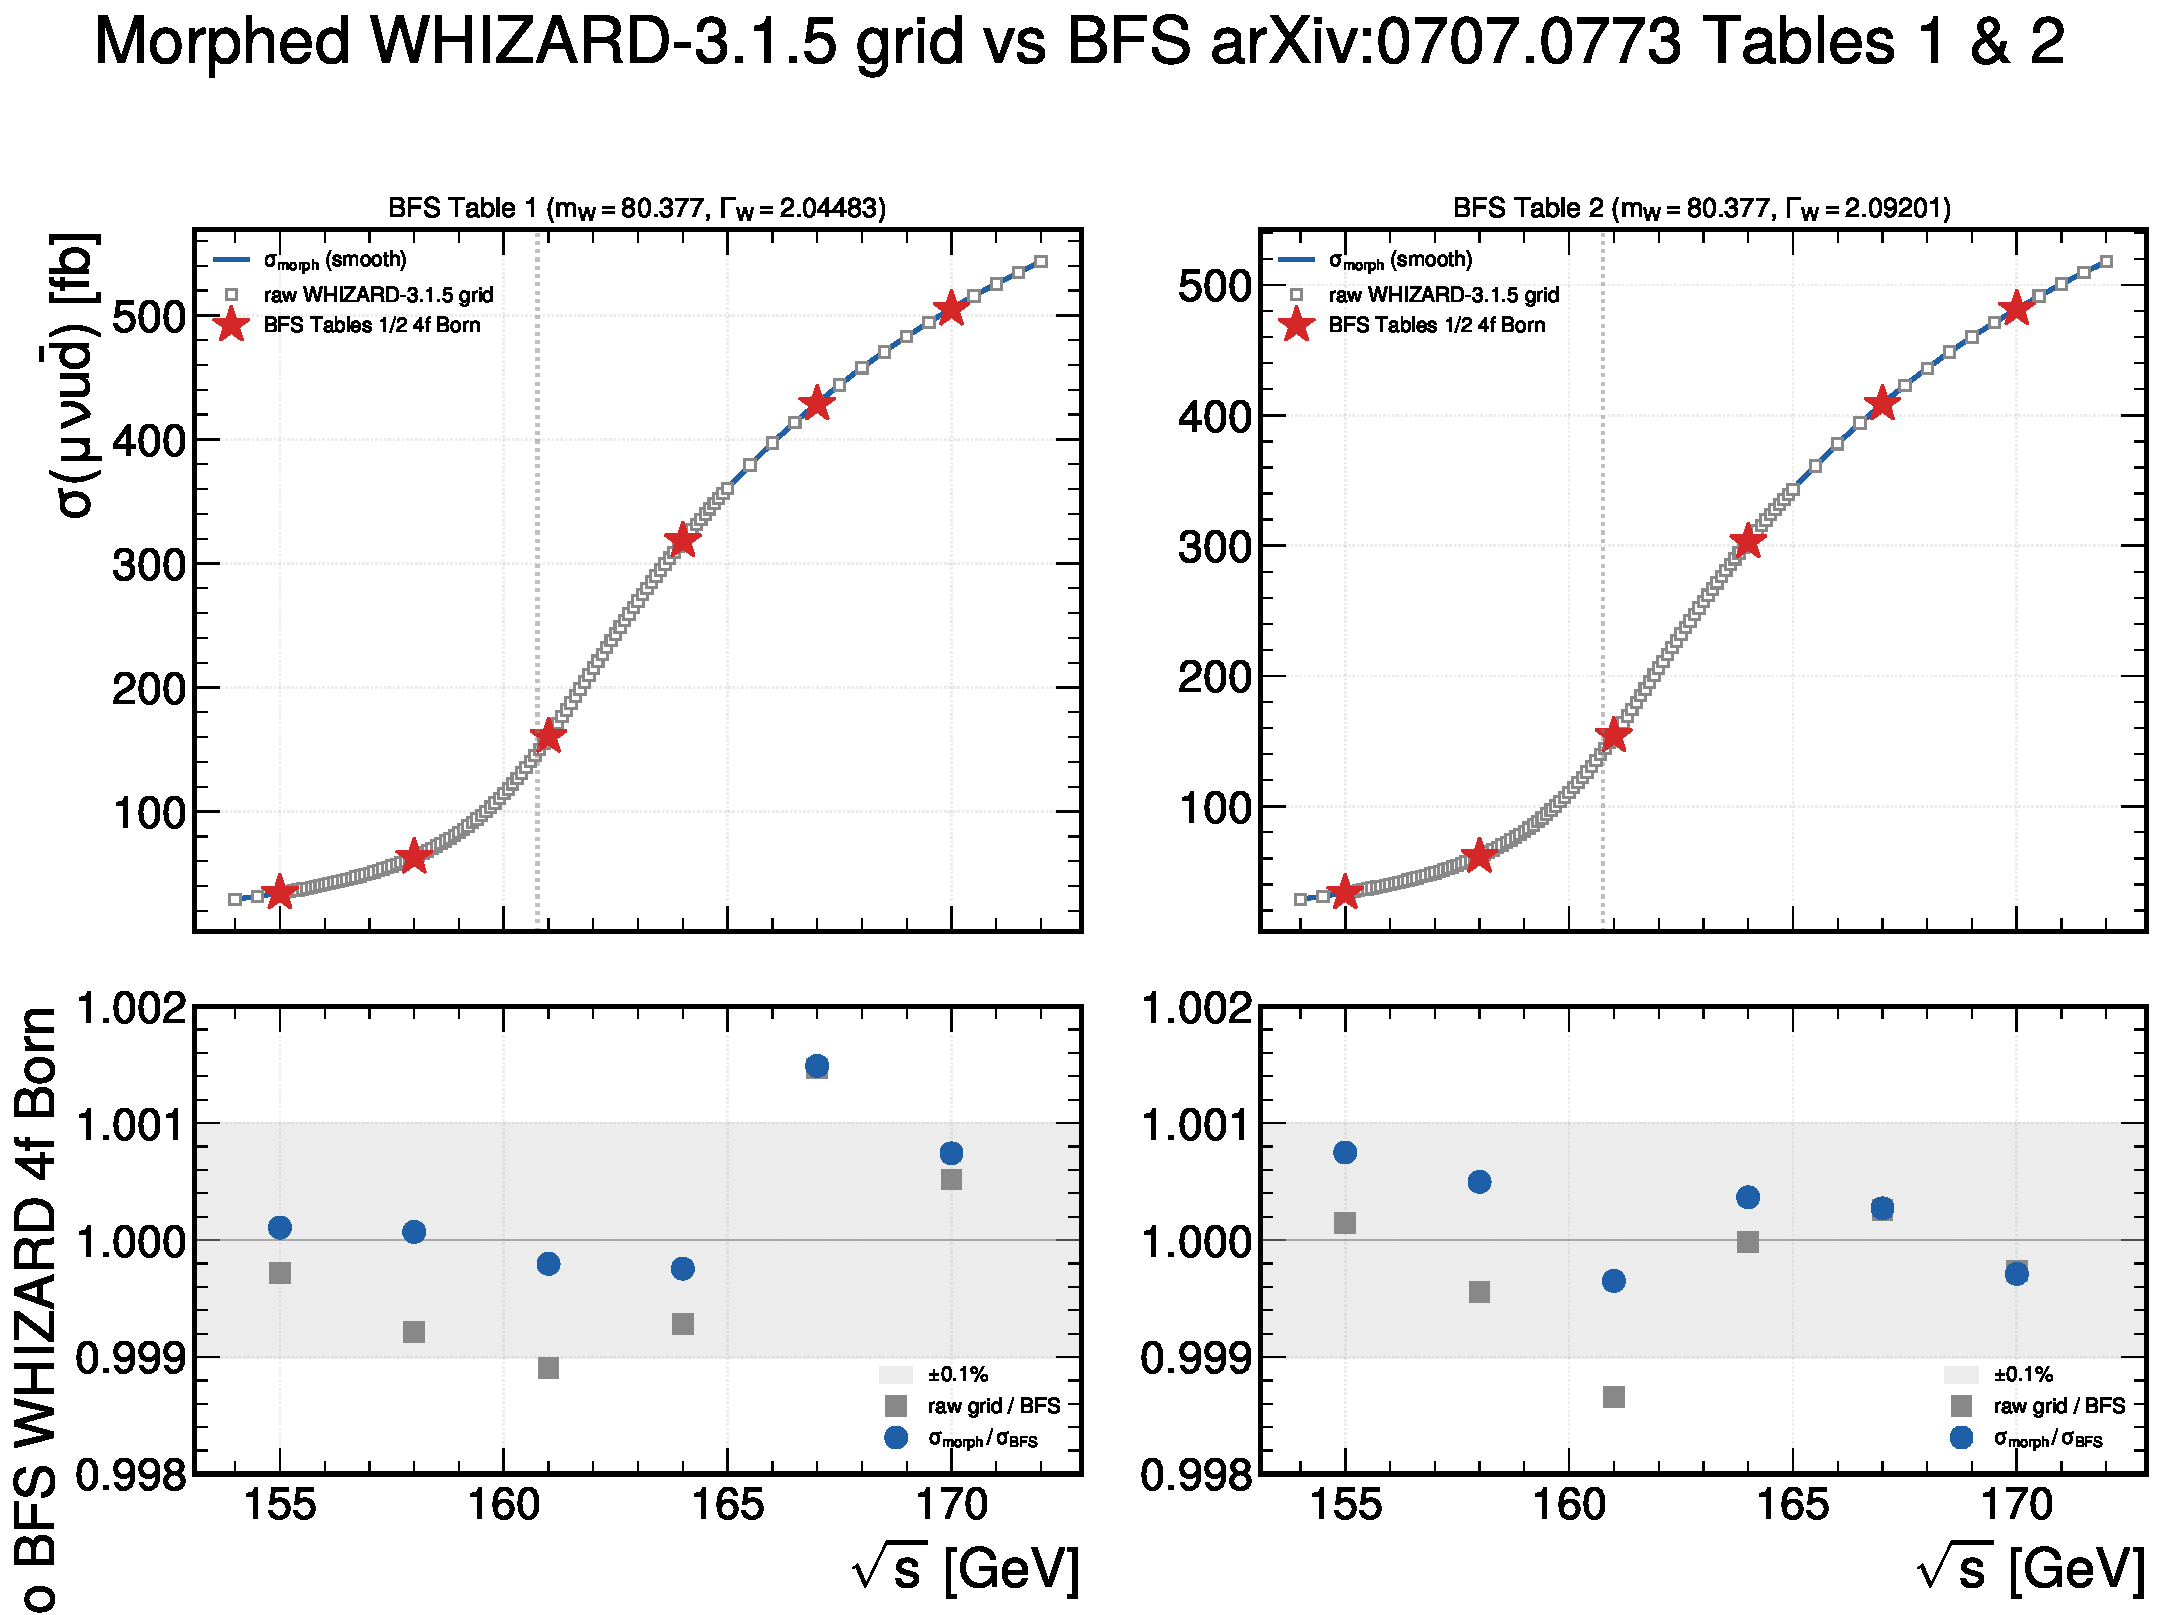
\includegraphics[width=0.88\linewidth]{morph_validate_bfs_tables}
\caption{External closure against BFS \cite{BFSnlo}. The morph is
evaluated at the BFS Table~1 ($\mW=80.377$, $\GammaW=2.04483\GeV$) and
Table~2 ($\mW=80.377$, $\GammaW=2.09201\GeV$) reference points and
compared with the paper's WHIZARD 4f Born column. Top: absolute
$\sigma(\sqrts)$ --- the morph curve, the raw grid and the BFS points
coincide. Bottom: the ratio to the BFS values. Agreement is
$<0.15\,\%$ at every $\sqrts$ (maximum $0.149\,\%$ on Table~1,
$0.075\,\%$ on Table~2); the morph/BFS ratio tracks the raw-grid/BFS
ratio closely, so the residual is the genuine
WHIZARD-3.1.5-versus-BFS-era generator difference and not a morph
interpolation error. This is the morphing analogue of the
single-anchor closure of section~\ref{sec:val-anchor}.}
\label{fig:mv-bfs}
\end{figure}

\subsection{Physics sanity}\label{sec:morphval-physics}

Finally, the morphed cross section is inspected as a physical line shape (Fig.~\ref{fig:mv-smooth}) and through the $\GammaW$-induced threshold crossing (Fig.~\ref{fig:mv-azzurri}).

\begin{figure}[htbp]
\centering
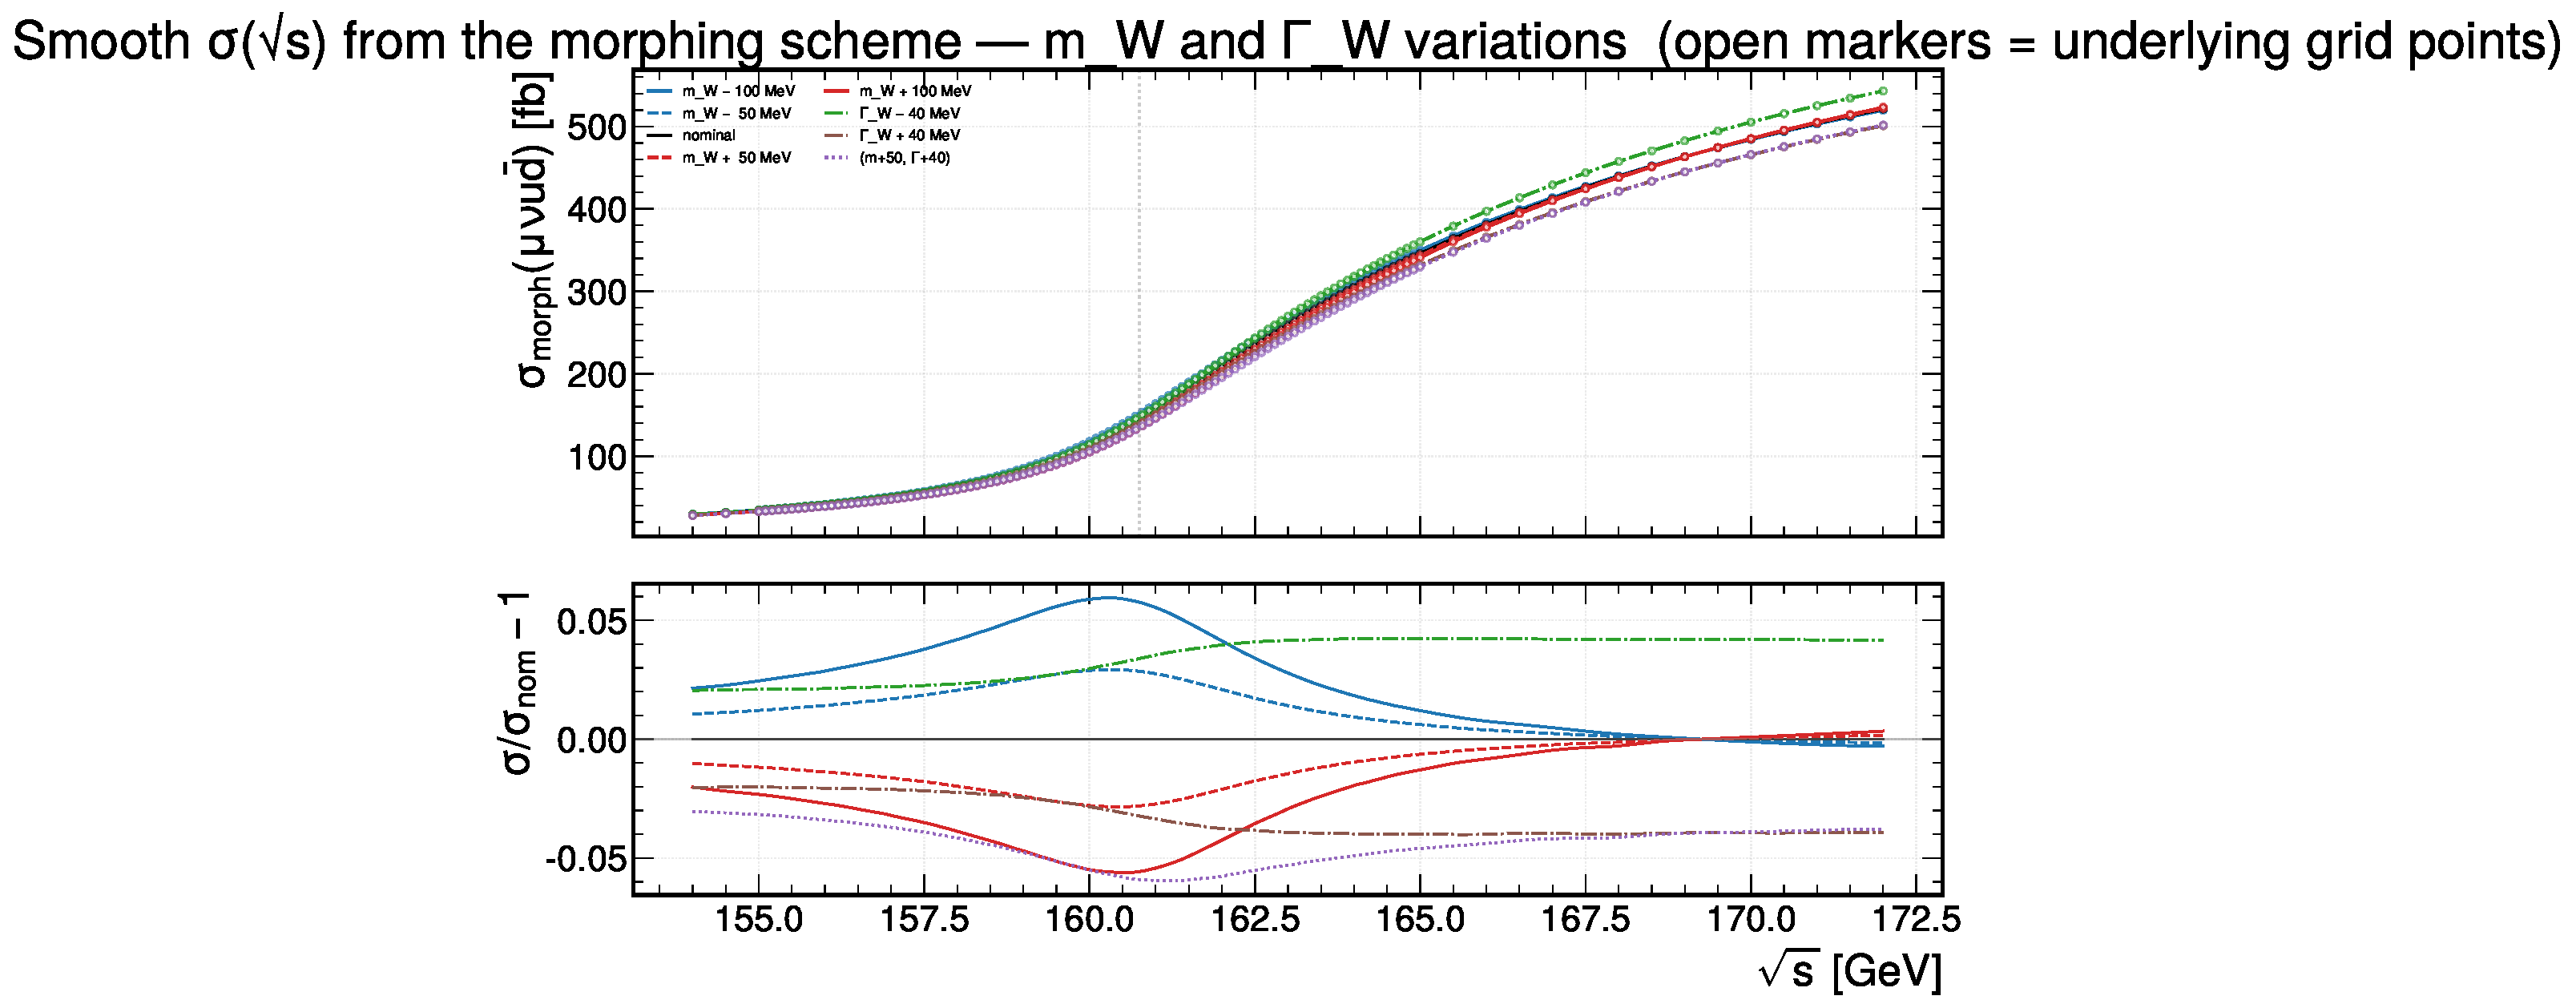
\includegraphics[width=0.82\linewidth]{morph_smooth_sigma_sqrts}
\caption{Smooth $\sigma(\sqrts)$ reconstructed from the morph for a set
of $\mW$ and $\GammaW$ variations around nominal; open markers are the
underlying grid points. Top: absolute $\sigma$. Bottom: ratio to the
nominal curve. The morph produces sensible, smooth threshold curves
between the grid $\sqrts$ knots for every variation.}
\label{fig:mv-smooth}
\end{figure}

\begin{figure}[htbp]
\centering
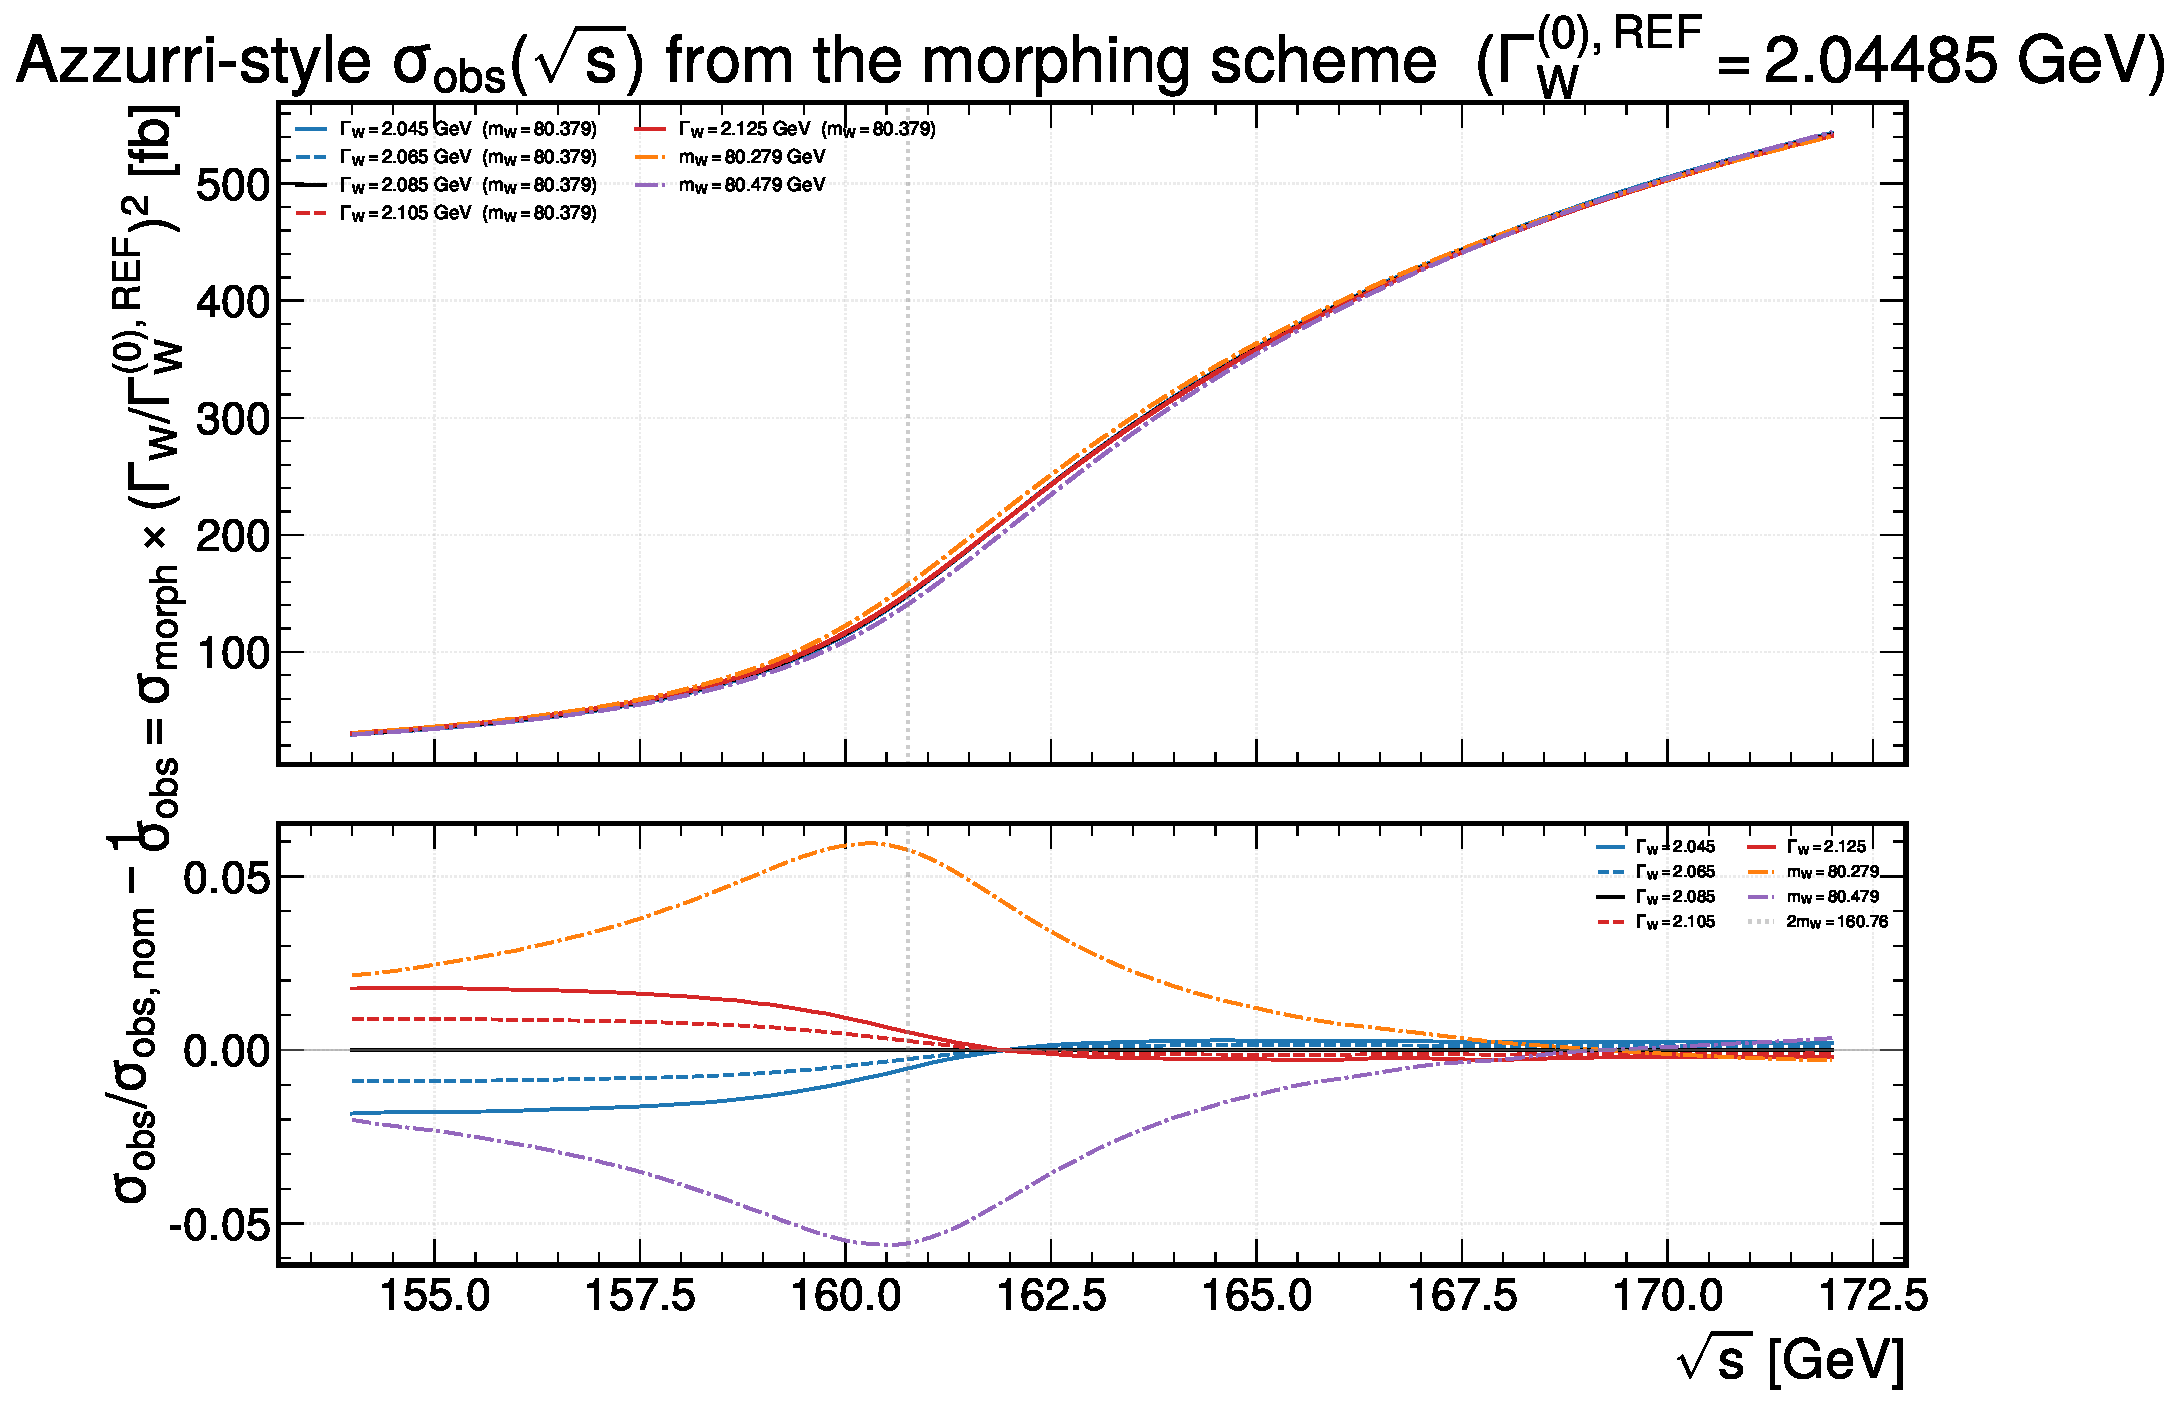
\includegraphics[width=0.82\linewidth]{morph_azzurri}
\caption{Azzurri-style $\sigma_\text{obs}(\sqrts)=
\sigma_\text{morph}\times(\GammaW/\Gamma_W^{(0),\mathrm{REF}})^2$ from
the morphing scheme. Top: absolute $\sigma_\text{obs}$ for $\GammaW$
and $\mW$ variations. Bottom: ratio to nominal, showing the
$\GammaW$-induced crossing at $\sqrts\simeq161.88\GeV$, consistent with
the $\sqrts\!\simeq\!162\GeV$ of Azzurri (\arxiv{2107.04444}); the
$\mW$ variations do not cross, as expected for the $\mW$-independent
PDG-constant BR factor.}
\label{fig:mv-azzurri}
\end{figure}

\clearpage
% ---------------------------------------------------------------
\section{$K_C$ decommission and the $K_C$-safe diagnostic alternative}\label{sec:kcsafe}
% ---------------------------------------------------------------

\paragraph{Decision (2026-05-26).} The production card now sets
\code{NLO_CONFIG["include_coulomb"]=False}: the Fadin--Khoze--Martin
Coulomb resummation factor $K_C$ is no longer multiplied onto the chain.
This appendix documents (i) why the previous $K_C\times\sigma$
combination is incorrect, (ii) what the K$_C$-safe knob
\code{NLO_CONFIG["coulomb_kc_safe"]} would have done as a partial
patch, and (iii) the numerical evidence behind the decommission.
The K$_C$-safe knob is retained as a card-level diagnostic alternative
for anyone wanting to recover the legacy $K_C$-on chain without the
leading-$\alpha/v$ double-count.

The Fadin--Khoze--Martin $K_C$ (\code{coulomb_K_factor}
in \code{eft_xsec.py}; refs:\ Fadin-Khoze-Martin, Phys.\ Lett.\ B 311
(1993) 311 and FKM-Stirling \cite{FKM1995}) is a LEP-era closed-form
multiplicative Coulomb resummation factor that predates the BFS
unstable-particle EFT formalism by roughly a decade. \emph{Neither BFS
paper uses it}: BFS treat the Coulomb correction via an
$\alpha$-expansion of the all-order Coulomb Green function
$G_C^{(0)}(0,0;E_W)$ (eq.~(61) of \cite{BFSnlo}, eq.~(9) of
\cite{BFSnnlo}); eq.~(62) of \cite{BFSnlo} is its
$\mathcal{O}(\alpha)+\mathcal{O}(\alpha^2)$ expansion. BFS explicitly
argue \emph{not} to resum the two-photon piece ($\sim$ few permille at
threshold; \cite{BFSnlo} lines 1722--1725) and add the eq.~(62)
contribution as an additive correction. The same Green-function
prescription is used throughout the PNRQCD tt-threshold literature
(Beneke et al.\ \arxiv{1506.06864}, Hoang-Stahlhofen
\arxiv{1309.6323}); no published EFT calculation uses a multiplicative
$K_C\times\sigma$ structure. Our framework's $K_C$ multiplier was a
pragmatic LEP-era engineering shortcut that survived into the BFS
chain assembly and double-counted the leading $\alpha/v$ Coulomb against
the BFS eq.~(62) addition. Dropping it brings the production chain
into the apples-to-paper configuration used in
section~\ref{sec:val-table4} (Scenario~F of \code{validate_bfs_nlo.py}).
A full $G_C$-based refactor (``Grade~B'' in the team memory) would
restore the all-order Coulomb resummation rigorously; until then we
accept BFS's $\sim 0.2\%$ unresummed-two-photon trade-off.

The technical details below are unchanged from the original K$_C$-safe
appendix and describe the partial-patch knob that survives in the
card for diagnostic comparisons.

\subsection*{The leading-$\alpha/v$ overlap (background)}

When $K_C$ is on, the BFS NLO Coulomb correction
$\Delta\sigma_\mathrm{Coul}^{(1)}$ of eq.~(62) of
\cite{BFSnlo} (\code{delta_sigma_Coulomb_NLO_specific_pb}, switched on
together with the rest of the NLO loop chain by
\code{NLO_CONFIG["include_NLO_hard_decay"]=True}) describes overlapping
physics on its leading-$\alpha/v$ piece. The first term of eq.~(62),
\begin{equation}
\Delta\sigma_{\mathrm{Coul}}^{(1),\,\mathrm{term\,1}}=
\frac{4\pi\alpha^2}{27 s_W^4 s}\,
\mathrm{Im}\!\left[-\frac{\alpha}{2}\ln\!\frac{-(E+i\GammaW)}{\mW}\right],
\qquad E=\sqrts-2\mW,
\end{equation}
is the unresummed first-order $\pi\alpha/v$ Coulomb correction of
\cite{FKM1995} eq.~(21) ($X/2\simeq +5.21\%$ at threshold), exactly
the leading-$\alpha/v$ piece that $K_C-1$ resums. With the framework's
off-shell-momentum prescription $K_C-1=+7.0\%$ at threshold; the
$\sim 2$\,pp offset to FKM's $X/2$ is the finite-$\GammaW$
regularisation chosen to keep $\sigma$ smooth in $(\mW,\GammaW)$.
Multiplying $K_C$ onto a $\sigma$ that already contains
$\Delta\sigma_{\mathrm{Coul}}^{(1),\,\mathrm{term\,1}}$ therefore
counts the leading Coulomb \emph{twice}. The second term of eq.~(62),
\begin{equation}
\Delta\sigma_{\mathrm{Coul}}^{(1),\,\mathrm{term\,2}}=
\frac{4\pi\alpha^2}{27 s_W^4 s}\,
\mathrm{Im}\!\left[\frac{\alpha^2\pi^2}{12}\sqrt{-\mW/(E+i\GammaW)}\right],
\end{equation}
is the two-photon $\alpha^2$ subleading piece
($X^2/6\simeq +0.17\%$ at threshold). It is not part of $K_C$'s
leading-$\alpha/v$ resummation and remains a genuine NLO correction
when $K_C$ is on.

\paragraph{The K$_C$-safe knob (diagnostic only).} A card knob
\code{NLO_CONFIG["coulomb_kc_safe"]} (default \texttt{False}; only
takes effect when \code{include_coulomb=True}) selects
between two interpretations of the eq.~(62) addition inside
\code{_add_nlo_loops_to_LR}, for users wishing to compare against the
historical $K_C$-on chain without the leading-$\alpha/v$ double-count:
\begin{itemize}
  \item \texttt{False} --- legacy $K_C$-on chain. The full eq.~(62)
    (term~1 $+$ term~2) is added on top of $K_C$. The
    leading-$\alpha/v$ Coulomb is double-counted at the $\sim 5\%$
    level on $\sigma$ at threshold. This chain is \emph{not} the
    production default (which has $K_C$ off) and has no direct BFS
    Table-4 cross-check.
  \item \texttt{True} --- $K_C$-safe. Eq.~(62) is added with the
    \code{subleading_only} flag, i.e.\ only term~2 (the
    $\alpha^2$ two-photon $\sim 0.2\%$) is retained. Combined with
    $K_C$, the chain avoids the leading-$\alpha/v$ double-count while
    keeping the genuine non-Coulomb NLO pieces (HSC and decay) and
    the subleading Coulomb correction beyond $K_C$. Still differs
    from the production K$_C$-off chain by the $\sim 2$\,pp off-shell
    prescription residual discussed below.
\end{itemize}
The knob is plumbed end-to-end through \code{sigma_partonic_munuqq}
(\code{eft_xsec.py}), \code{sigma_observed_munuqq} (\code{isr.py}), and
\code{WWGenerator.template_fingerprint} --- the freshness check in
\code{doFit_ww.py} therefore aborts the fit if the templates were
generated under a different setting than the live card.

\paragraph{Validation.} Four cross-checks under
\code{scripts/investigations/coulomb_double_count/} pin the
implementation:
\begin{itemize}
\item \textbf{Route-A vs Route-B identity.} The two-call difference
  $\sigma(\texttt{kcsafe}{=}\mathrm{False}) -
   \sigma(\texttt{kcsafe}{=}\mathrm{True})$ from the chain matches the
  standalone term-1 piece
  $\Delta\sigma_{\mathrm{Coul}}^{(1),\,\mathrm{term\,1}}$ assembled
  directly from the helper, with the appropriate $27/4$
  specific-to-total factor (and $\times\delta_\mathrm{QCD}$ when
  active). Max relative error $3.4\times 10^{-15}$ without
  $\delta_\mathrm{QCD}$, $5.1\times 10^{-15}$ with --- machine
  precision.
\item \textbf{Same-physics overlap.} $K_C-1$ and
  $\Delta\sigma_{\mathrm{Coul}}^{(1),\,\mathrm{term\,1}}/\sigma_{LR}^{(0)}$
  are both $\sim 5{-}7\%$ at threshold, fall to $\sim 3\%$ at
  $\sqrts=172\GeV$, and track each other with a near-constant
  $\sim {+}2$\,pp offset --- two formulations of the same physics.
\item \textbf{FKM 1995 strict near-threshold.} At
  $\sqrts=2\,M_W^{\mathrm{BFS\,ref}}=160.754\GeV$, the standalone
  term-1 piece evaluates to $+5.27\%$ on $\sigma_{LR}^{(0)}$ vs FKM's
  $X/2=+5.21\%$ --- agreement at the $1\%$ relative level.
\item \textbf{Legacy-chain magnitude.} Relative to the legacy
  $K_C$-on chain (PDG-constant BR, full NLO$+$NNLO,
  $\delta_\mathrm{QCD}$, Whizard anchor), the $K_C$-safe combination
  reduces $\sigma_\mathrm{partonic}$ by $-7.9\%$ at $\sqrts=157\GeV$,
  $-7.7\%$ at $161\GeV$, $-6.5\%$ at $163\GeV$. The shift is smooth in
  $\sqrts$ with no new kinks;
  $\mathrm{d}\sigma/\mathrm{d}\mW$ and $\mathrm{d}\sigma/\mathrm{d}\GammaW$
  retain the same overall shape (Fig.~\ref{fig:kcsafe-chain}). The
  production K$_C$-off default sits a further $\sim 2$\,pp below the
  K$_C$-safe curve at threshold (see Fig.~\ref{fig:kcsafe-overlap}
  and the structural discussion above).
\end{itemize}

The same-physics overlap of $K_C-1$ and
$\Delta\sigma_{\mathrm{Coul}}^{(1),\,\mathrm{term\,1}}/\sigma_{LR}^{(0)}$
is shown in Fig.~\ref{fig:kcsafe-overlap}; the bottom panel makes the
$\sim 2$\,pp off-shell prescription offset explicit. The two-photon
$\alpha^2$ subleading piece (grey curve in the top panel) stays below
$0.2\%$ throughout, justifying its treatment as a genuine NLO
correction beyond $K_C$. The Route-A/Route-B identity is summarised
in Tab.~\ref{tab:kcsafe-identity}.

\begin{figure}[htbp]
\centering
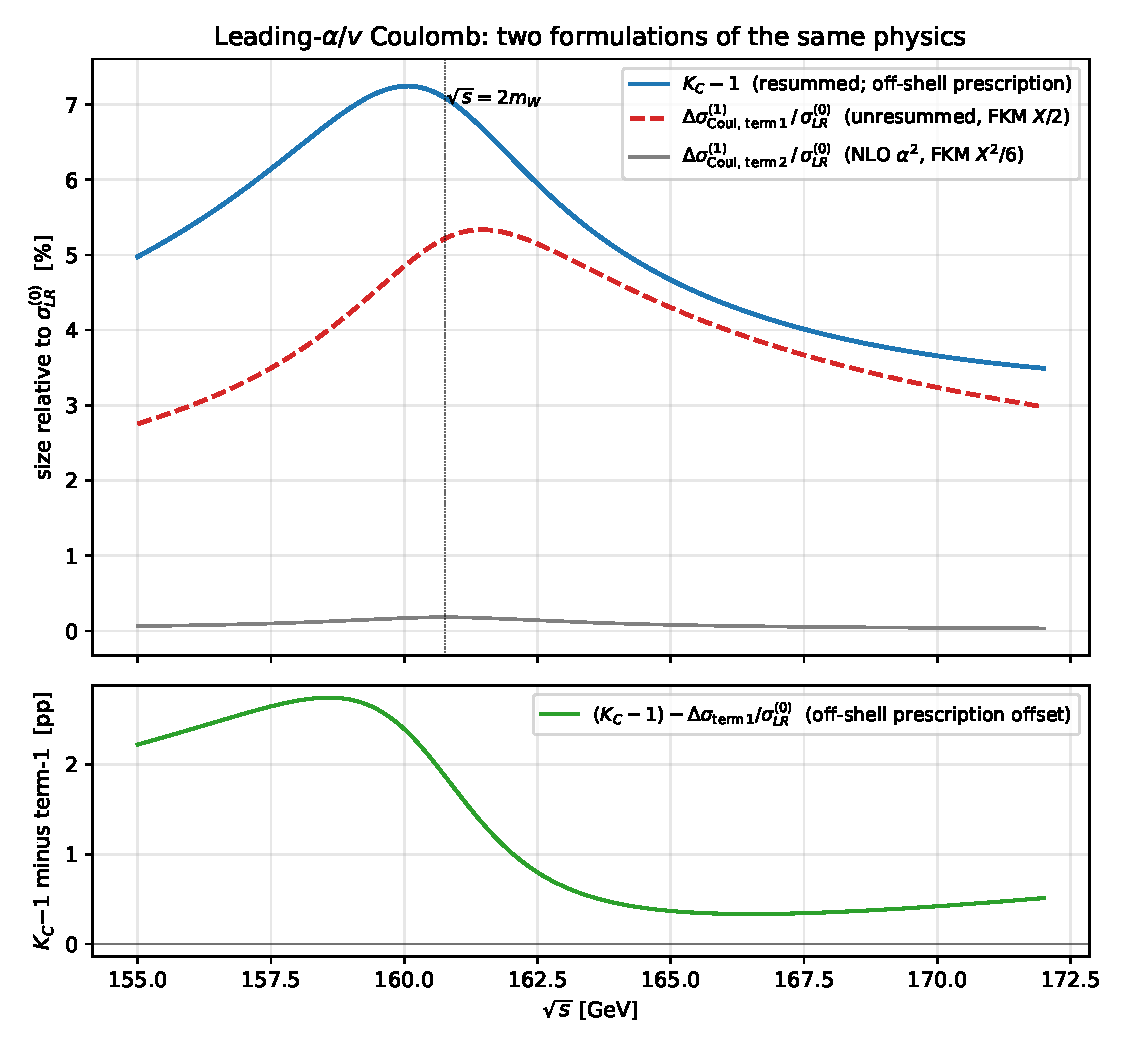
\includegraphics[width=0.82\linewidth]{coul_kc_vs_term1_overlap}
\caption{Top: the Fadin-Khoze-Martin resummation $K_C-1$ (blue) and
the first term of BFS eq.~(62)
$\Delta\sigma_{\mathrm{Coul}}^{(1),\,\mathrm{term\,1}}/\sigma_{LR}^{(0)}$
(red, dashed) are two formulations of the same leading-$\alpha/v$
Coulomb physics, both $\sim 5{-}7\%$ at threshold and falling above.
The framework's complex-$p$ regularisation gives $K_C-1$ a $\sim 2$\,pp
upward offset (bottom panel) over the unresummed FKM $X/2$ near
threshold, with the offset shrinking to $\sim 0.4$\,pp above $\sqrts=
165\GeV$. The genuine NLO $\alpha^2$ two-photon piece
$\Delta\sigma_{\mathrm{Coul}}^{(1),\,\mathrm{term\,2}}/\sigma_{LR}^{(0)}$
(grey) is sub-permil throughout and is what the $K_C$-safe combination
retains in eq.~(62). Produced by
\code{scripts/investigations/coulomb_double_count/plot_kc_vs_term1_overlap.py}.}
\label{fig:kcsafe-overlap}
\end{figure}

\begin{table}[htbp]
\centering
\caption{Route-A vs Route-B closure for the $K_C$-safe knob,
$\sigma_\mathrm{BFS,\,total\,WW}$ at $\mW=80.379\GeV$, $\GammaW=2.085\GeV$,
no $\delta_\mathrm{QCD}$. \emph{Chain diff}: from two calls of
\code{sigma_BFS_LO_total_WW_pb} with
\code{coulomb_kc_safe} $=\{$False$, $True$\}$. \emph{Closed form}:
the same number assembled directly from the eq.~(62) helper,
$(27/4)\times[\Delta\sigma^{(1)}_{\mathrm{Coul}}({\tt subleading\_only=False})
-\Delta\sigma^{(1)}_{\mathrm{Coul}}({\tt subleading\_only=True})]$.
Machine precision throughout.}
\label{tab:kcsafe-identity}
\begin{tabular}{r r r r}
\toprule
$\sqrts$ [GeV] & chain diff [pb] & closed form [pb] & rel.\ err.\\
\midrule
155.00 & $+7.69984\times 10^{-2}$ & $+7.69984\times 10^{-2}$ & $-1.3\times 10^{-15}$\\
157.00 & $+1.09421\times 10^{-1}$ & $+1.09421\times 10^{-1}$ & $+2.5\times 10^{-16}$\\
160.00 & $+2.54191\times 10^{-1}$ & $+2.54191\times 10^{-1}$ & $-1.1\times 10^{-15}$\\
161.00 & $+3.46408\times 10^{-1}$ & $+3.46408\times 10^{-1}$ & $-1.4\times 10^{-15}$\\
162.50 & $+4.57089\times 10^{-1}$ & $+4.57089\times 10^{-1}$ & $+3.4\times 10^{-15}$\\
165.00 & $+5.25086\times 10^{-1}$ & $+5.25086\times 10^{-1}$ & $+1.1\times 10^{-15}$\\
168.00 & $+5.39801\times 10^{-1}$ & $+5.39801\times 10^{-1}$ & $+2.5\times 10^{-15}$\\
172.00 & $+5.32434\times 10^{-1}$ & $+5.32434\times 10^{-1}$ & $-4.2\times 10^{-16}$\\
\bottomrule
\end{tabular}
\end{table}

\begin{figure}[htbp]
\centering
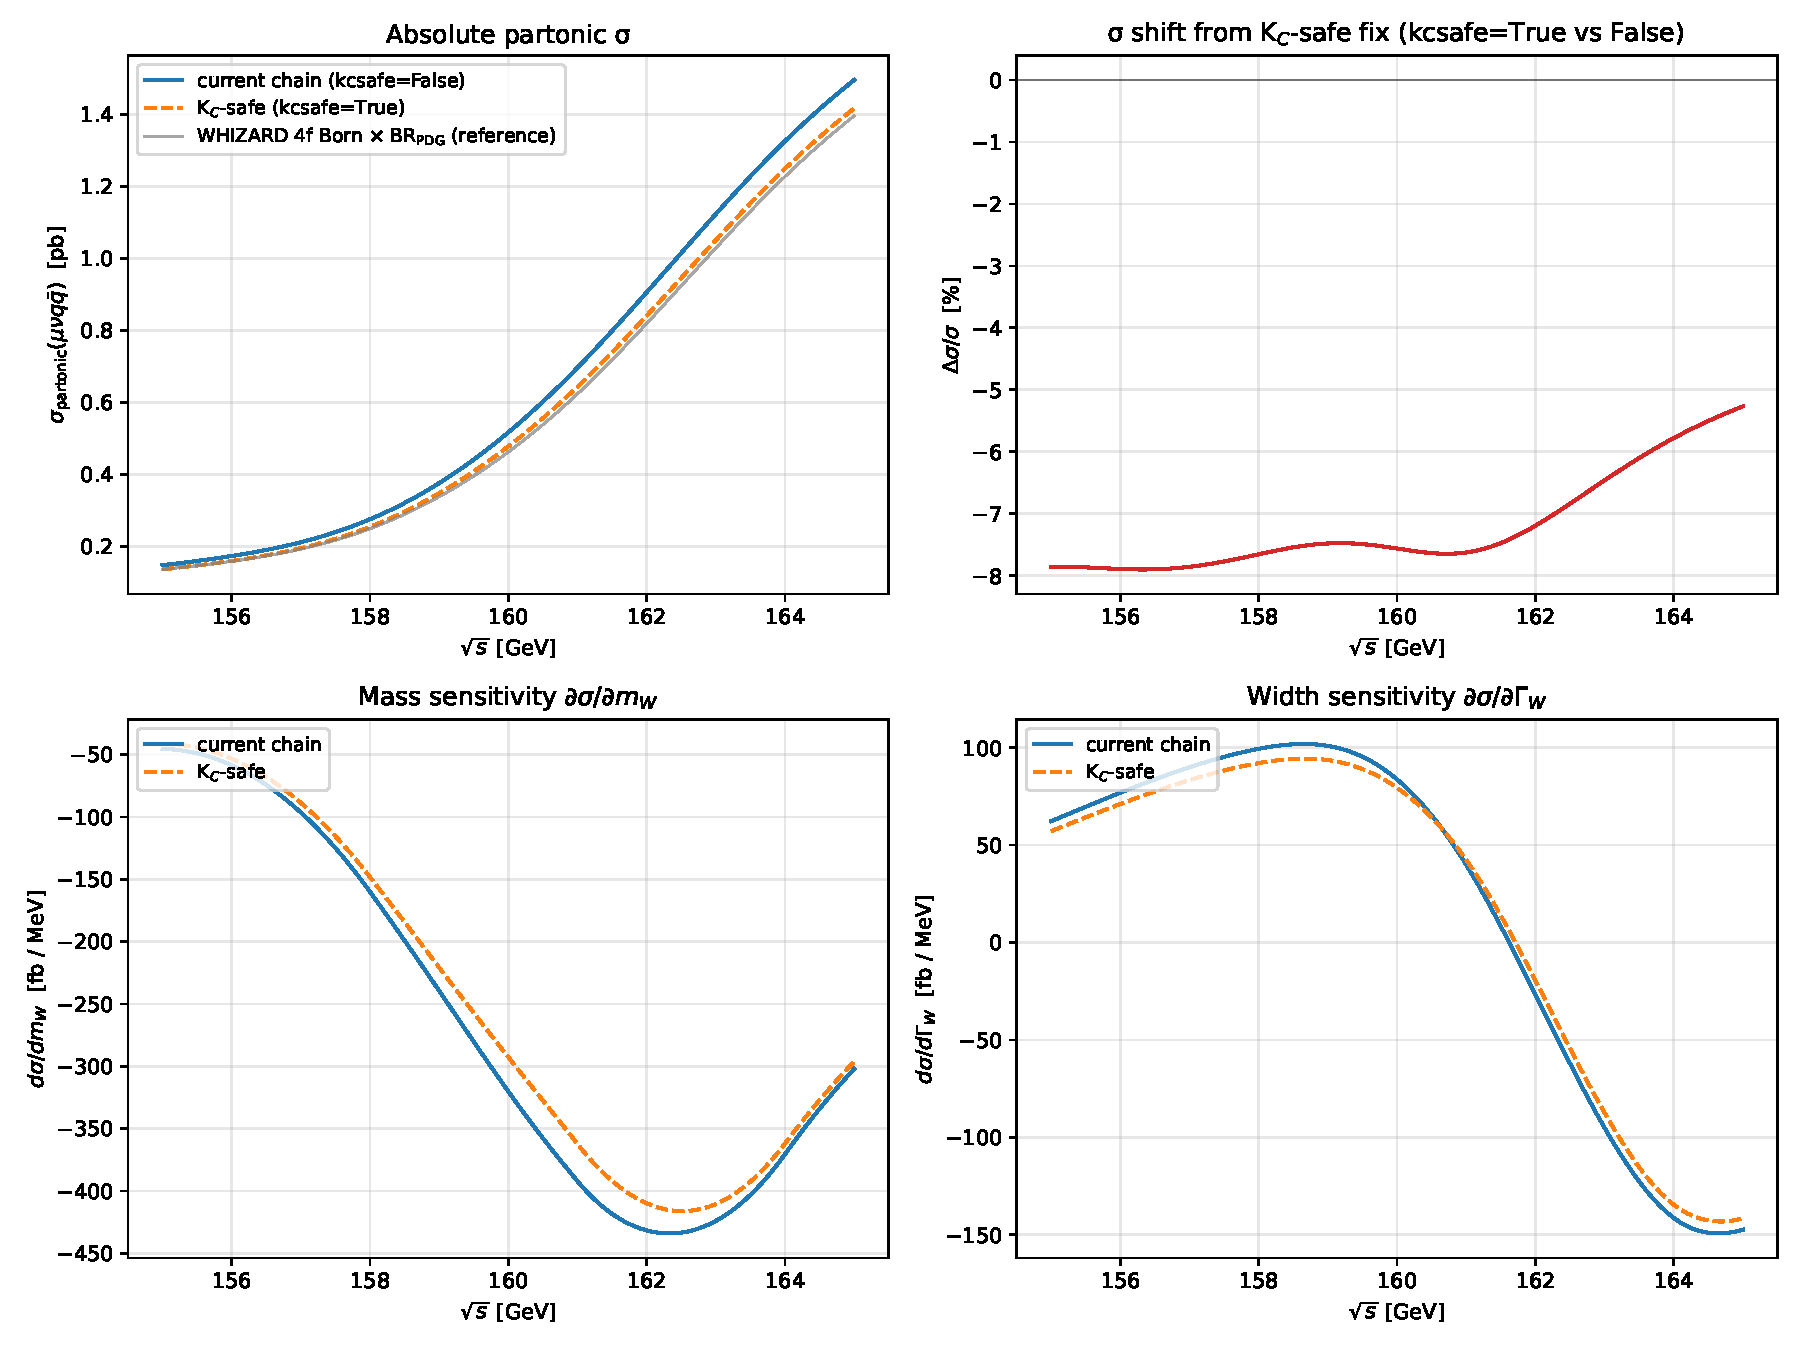
\includegraphics[width=0.93\linewidth]{coul_compare_kc_safe_chain}
\caption{Production-chain impact of the $K_C$-safe knob at the default
configuration (PDG-constant BR, full NLO$+$NNLO, $\delta_\mathrm{QCD}$,
spline anchor; partonic, no ISR). \emph{Top-left}: absolute $\sigma$
with the current chain (\code{coulomb_kc_safe=False}, blue) and the
$K_C$-safe alternative (orange, dashed); the WHIZARD 4f Born reference
$\sigma_\mathrm{Born}\times\mathrm{BR}_\mathrm{PDG}$ overlays in grey.
\emph{Top-right}: relative shift $\sigma_{K_C\text{-safe}}/\sigma_\mathrm{current}
- 1$ in percent --- a smooth $\sim -8\%$ at threshold dropping to
$\sim -5\%$ at $\sqrts=170\GeV$. \emph{Bottom row}:
$\mathrm{d}\sigma/\mathrm{d}\mW$ (left) and
$\mathrm{d}\sigma/\mathrm{d}\GammaW$ (right) computed by central
finite difference at $\mW=80.379\GeV$, $\GammaW=2.085\GeV$. The
derivative shapes are preserved; no new kink is introduced. Produced
by \code{scripts/investigations/coulomb_double_count/compare_anchor_before_after.py}.}
\label{fig:kcsafe-chain}
\end{figure}

\paragraph{Fit impact (Asimov A/B).} A clean A/B was performed on
2026-05-26 by regenerating both K$_C$-on and K$_C$-off templates with
the current chain (commit 82c7f1d, post the Table~2 BR-correction fix)
and running \code{doFit_ww.py} (default FCC-ee scenario) plus
\code{scripts.fit_2107_04444_scenario} against each. Results below.

\begin{table}[h]
\centering
\caption{Asimov A/B comparing the new K$_C$-off production default
against the legacy K$_C$-on chain, on two fit configurations
(both with the current Born + NLO + NNLO + $\delta_\mathrm{QCD}$ +
Whizard-anchor + LL+exp ISR chain). $\Delta\mW$ is the statistical
$\mW$ uncertainty; $\rho(\mW,\GammaW)$ the post-fit correlation.}
\label{tab:kcsafe-ab}
\begin{tabular}{l r r r}
\toprule
configuration & $\Delta\mW$ [MeV] & $\rho(\mW,\GammaW)$ & $\mW$ pull \\
\midrule
\multicolumn{4}{l}{\emph{Default FCC-ee scenario}, \code{doFit_ww.py}:} \\
~~legacy ($K_C$ on)   & 1.76 & $+0.61$ & 0.148 \\
~~production ($K_C$ off) & 1.80 & $+0.63$ & 0.147 \\
\midrule
\multicolumn{4}{l}{\emph{Azzurri 2107.04444 scenario}:} \\
~~legacy ($K_C$ on)   & 2.44 & $+0.58$ & 0.115 \\
~~production ($K_C$ off) & 2.44 & $+0.58$ & 0.115 \\
\bottomrule
\end{tabular}
\end{table}

\noindent
Asimov closure is preserved by both chains. Dropping $K_C$ shifts
$\Delta\mW$ by $+0.04\MeV$ on the default FCC-ee scenario (well
sub-MeV) and by $0\MeV$ on the Azzurri scenario; $\rho(\mW,\GammaW)$
shifts by $+0.02$ on the default scenario, by $0$ on the Azzurri
scenario. The luminosity nuisance fully absorbs the constant
$\Delta\sigma/\sigma \sim 5{-}8\%$ between the two chains across the
scan; the residual $\sim 0.3\%$ shape slope is too small to register
at the precision of these Asimov fits. The $\mW$ central value
recovered from the pseudodata is identical to 6-digit precision in
all four runs.

\paragraph{Verdict.} Grade~A is safe to ship: dropping $K_C$
preserves Asimov closure, leaves the m\textsubscript{W} central value
unchanged, and changes the statistical uncertainty by less than
$0.05\MeV$. The Grade~B G$_C$-based refactor (project memory) is a
nice-to-have publication upgrade rather than a bug fix, and can be
scheduled behind the parallel-implementation cross-check.

\paragraph{What the morphing scheme sees.} The WHIZARD Born anchor
$f(\delta,\GammaW)$ of section~\ref{sec:anchor} and
Appendix~\ref{sec:morphval} is a Born-level matching factor
$\sigma_\mathrm{WHIZARD}/\sigma_\mathrm{BFS-EFT,\,Born}$; it does not
depend on $K_C$, NLO loops, or the \code{coulomb_kc_safe} setting,
so dropping $K_C$ from the chain does not require any morph
regeneration.

% ---------------------------------------------------------------
\begin{thebibliography}{9}
% ---------------------------------------------------------------

\bibitem{BFSnlo}
M.~Beneke, P.~Falgari, C.~Schwinn, A.~Signer and G.~Zanderighi,
\emph{Four-fermion production near the W pair production threshold},
Nucl.\ Phys.\ B \textbf{792} (2008) 89--135,
\arxiv{0707.0773}.

\bibitem{BFSnnlo}
S.~Actis, M.~Beneke, P.~Falgari and C.~Schwinn,
\emph{Dominant NNLO corrections to four-fermion production near the
W-pair production threshold},
Nucl.\ Phys.\ B \textbf{807} (2009) 1--32,
\arxiv{0807.0102}.

\bibitem{FKM1995}
V.S.~Fadin, V.A.~Khoze, A.D.~Martin and W.J.~Stirling,
\emph{Threshold behaviour of the
$e^+e^-\!\to W^+W^-$ cross section},
Phys.\ Lett.\ B \textbf{363} (1995) 112--118,
\arxiv{hep-ph/9507422}.

\bibitem{LEP2YRww}
W.~Beenakker, F.A.~Berends et al.,
\emph{WW cross sections and distributions},
in \emph{Physics at LEP2}, eds.\ G.~Altarelli and F.~Zwirner,
CERN Yellow Report CERN 96-01 (1996),
\arxiv{hep-ph/9602351}.

\bibitem{Skrzypek1992}
M.~Skrzypek,
\emph{Leading logarithmic calculations of QED corrections at LEP},
Acta Phys.\ Polon.\ B \textbf{23} (1992) 135--172.

\bibitem{CDMN1992}
M.~Cacciari, A.~Deandrea, G.~Montagna and O.~Nicrosini,
\emph{QED structure functions: a systematic approach},
Europhys.\ Lett.\ \textbf{17} (1992) 123.

\end{thebibliography}

\end{document}
